\documentclass{article}
\usepackage[backend=biber,natbib=true,style=alphabetic,maxbibnames=50]{biblatex}
\addbibresource{/home/nqbh/reference/bib.bib}
\usepackage[utf8]{vietnam}
\usepackage{tocloft}
\renewcommand{\cftsecleader}{\cftdotfill{\cftdotsep}}
\usepackage[colorlinks=true,linkcolor=blue,urlcolor=red,citecolor=magenta]{hyperref}
\usepackage{amsmath,amssymb,amsthm,float,graphicx,mathtools,tikz}
\usepackage{enumitem}
\setlist{leftmargin=4mm}
\usetikzlibrary{angles,calc,intersections,matrix,patterns,quotes,shadings}
\allowdisplaybreaks
\newtheorem{assumption}{Assumption}
\newtheorem{baitoan}{}%{Bài toán}
\newtheorem{cauhoi}{Câu hỏi}
\newtheorem{conjecture}{Conjecture}
\newtheorem{corollary}{Corollary}
\newtheorem{dangtoan}{Dạng toán}
\newtheorem{definition}{Definition}
\newtheorem{dinhly}{Định lý}
\newtheorem{dinhnghia}{Định nghĩa}
\newtheorem{example}{Example}
\newtheorem{ghichu}{Ghi chú}
\newtheorem{hequa}{Hệ quả}
\newtheorem{hypothesis}{Hypothesis}
\newtheorem{lemma}{Lemma}
\newtheorem{luuy}{Lưu ý}
\newtheorem{nhanxet}{Nhận xét}
\newtheorem{notation}{Notation}
\newtheorem{note}{Note}
\newtheorem{principle}{Principle}
\newtheorem{problem}{Problem}
\newtheorem{proposition}{Proposition}
\newtheorem{question}{Question}
\newtheorem{remark}{Remark}
\newtheorem{theorem}{Theorem}
\newtheorem{vidu}{Ví dụ}
\usepackage[left=1cm,right=1cm,top=5mm,bottom=5mm,footskip=4mm]{geometry}
\def\labelitemii{$\circ$}
\DeclareRobustCommand{\divby}{%
	\mathrel{\vbox{\baselineskip.65ex\lineskiplimit0pt\hbox{.}\hbox{.}\hbox{.}}}%
}

\title{Problem: Root -- Bài Tập: Căn Thức}
\author{Nguyễn Quản Bá Hồng\footnote{Independent Researcher, Ben Tre City, Vietnam\\e-mail: \texttt{nguyenquanbahong@gmail.com}; website: \url{https://nqbh.github.io}.}}
\date{\today}

\begin{document}
\maketitle
\begin{abstract}
	Last updated version: \href{https://github.com/NQBH/elementary_STEM_beyond/blob/main/elementary_mathematics/grade_9/root/problem/NQBH_root_problem.pdf}{GitHub{\tt/}NQBH{\tt/}elementary STEM \& beyond{\tt/}elementary mathematics{\tt/}grade 9{\tt/}root{\tt/}problem: set $\mathbb{Q}$ of roots [pdf]}.\footnote{\textsc{url}: \url{https://github.com/NQBH/elementary_STEM_beyond/blob/main/elementary_mathematics/grade_9/root/problem/NQBH_root_problem.pdf}.} [\href{https://github.com/NQBH/elementary_STEM_beyond/blob/main/elementary_mathematics/grade_9/root/problem/NQBH_root_problem.tex}{\TeX}]\footnote{\textsc{url}: \url{https://github.com/NQBH/elementary_STEM_beyond/blob/main/elementary_mathematics/grade_9/rational/problem/NQBH_root_problem.tex}.}. 
\end{abstract}
\tableofcontents

%------------------------------------------------------------------------------%

\section{Căn Bậc 2 \& Số Vô Tỷ}
Ở Toán 7 (xem, e.g., \cite[\S5, pp. 27--29]{SGK_Toan_7_Canh_Dieu_tap_1}), ta đã biết dạng biểu diễn thập phân của số hữu tỷ là hữu hạn hoặc vô hạn tuần hoàn, dạng biểu diễn thập phân của số vô tỷ là vô hạn không tuần hoàn. Số hữu tỷ $a\in\mathbb{Q}$ nào cũng viết được dưới dạng $a = \dfrac{m}{n}$ với $m\in\mathbb{Z}$, $n\in\mathbb{N}^\star$.

\noindent\cite[Chap. III, \S1, pp. 48--54]{SGK_Toan_9_Canh_Dieu_tap_1}: HD1. LT1. HD2. LT2. HD3. LT3. 1. 2. 3. 4. 5. 6. 7. 8. 9.

\section{Square Root \& Irrationals -- Căn Bậc 2 \& Số Vô Tỷ}

\begin{baitoan}[\cite{SGK_Toan_9_tap_1}, ?1--?3, pp. 4--5]
	(a) Tìm các căn bậc 2 của $9,\frac{4}{9},0.25,2$. (b) Tìm căn bậc 2 số học của $49,64,81,1.21$. (c) Tìm căn bậc 2 của $49,64,81,1.21$.
\end{baitoan}

\begin{baitoan}[\cite{SGK_Toan_9_tap_1}, Ví dụ 2, ?4, pp. 5--6]
	So sánh: (a) $1$ \& $\sqrt{2}$. (b) $2$ \& $\sqrt{5}$. (c) $4$ \& $\sqrt{15}$. (d) $\sqrt{11}$ \& $3$.
\end{baitoan}

\begin{baitoan}[\cite{SGK_Toan_9_tap_1}, Ví dụ 3, ?5, p. 6]
	(a) Tìm $x\in\mathbb{R}$ thỏa: (a) $\sqrt{x} > 2$. (b) $\sqrt{x} < 1$. (c) $\sqrt{x} > 1$. (d) $\sqrt{x} < 3$.
\end{baitoan}

\begin{baitoan}[\cite{SGK_Toan_9_tap_1}, 1., p. 6]
	Tìm căn bậc 2 số học của mỗi số sau rồi suy ra căn bậc 2 của chúng: \emph{121, 144, 169, 225, 256, 324, 361, 400}.
\end{baitoan}

\begin{baitoan}[\cite{SGK_Toan_9_tap_1}, 2., p. 6]
	So sánh: (a) $2$ \& $\sqrt{3}$. (b) $6$ \& $\sqrt{41}$. (c) $7$ \& $\sqrt{47}$.
\end{baitoan}

\begin{baitoan}[\cite{SGK_Toan_9_tap_1}, 3., p. 6]
	Tìm $x\in\mathbb{R}$ thỏa mãn các phương trình sau \& sau đó làm tròn đến chữ số thập phân thứ 3: (a) $x^2 = 2$. (b) $x^2 = 3$. (c) $x^2 = 3.5$. (d) $x^2 = 4.12$.
\end{baitoan}
\noindent{\sf Hint.} Nghiệm của phương trình bậc 2 $x^2 = a$ với $a\ge0$ là các căn bậc 2 của $a$.

\begin{baitoan}[\cite{SGK_Toan_9_tap_1}, 4., p. 7]
	Tìm $x\in\mathbb{R}$ thỏa: (a) $\sqrt{x} = 15$. (b) $2\sqrt{x} = 14$. (c) $\sqrt{x} < \sqrt{2}$. (d) $\sqrt{2x} < 4$.
\end{baitoan}

\begin{baitoan}[\cite{SGK_Toan_9_tap_1}, 5., p. 7]
	Tính cạnh 1 hình vuông biết diện tích của nó bằng diện tích của hình chữ nhật có chiều rộng \emph{3.5 m} \& chiều dài \emph{14 m}.
\end{baitoan}

\begin{baitoan}[\cite{SBT_Toan_9_tap_1}, 1., p. 5]
	Tính căn bậc 2 số học của \emph{0.01, 0.04, 0.49, 0.64, 0.25, 0.81, 0.09, 0.16, 0, $-1$.}
\end{baitoan}

\begin{proof}[Giải]
	Căn bậc 2 số học của: 0.01, 0.04, 0.49, 0.64, 0.25, 0.81, 0.09, 0.16, 0 lần lượt là $\sqrt{0.01} = 0.1$, $\sqrt{0.04} = 0.2$, $\sqrt{0.49} = 0.7$, $\sqrt{0.64} = 0.8$, $\sqrt{0.25} = 0.5$, $\sqrt{0.81} = 0.9$, $\sqrt{0.09} = 0.3$, $\sqrt{0.16} = 0.4$, $\sqrt{0} = 0$. Riêng $-1$ không có căn bậc 2 (số học) vì $-1 < 0$.
\end{proof}

\begin{luuy}
	Căn bậc 2 số học của số thực không âm $a\ge0$ là $\sqrt{a}$. Căn bậc 2 của $a\ge0$ là $\pm\sqrt{a}$ (i.e., bao gồm $\sqrt{a}$ \& $-\sqrt{a}$), đặc biệt: căn bậc 2 của $0$ là $\pm\sqrt{0} = 0$. Mọi số thực âm $a < 0$ không có căn bậc 2. 
\end{luuy}

\begin{baitoan}[\cite{SBT_Toan_9_tap_1}, 2., p. 5]
	Tìm $x\in\mathbb{R}$ thỏa: (a) $x^2 = 5$. (b) $x^2 = 6$. (c) $x^2 = 2.5$. (d) $x^2 = \sqrt{5}$. (e) $x^2 = -1$.
\end{baitoan}

\begin{proof}[Giải]
	(a) $x^2 = 5\Leftrightarrow x = \pm\sqrt{5}$. (b) $x^2 = 6\Leftrightarrow x = \pm\sqrt{6}$. (c) $x^2 = 2.5\Leftrightarrow x = \pm\sqrt{2.5}$. (d) $x^2 = \sqrt{5}\Leftrightarrow x = \pm\sqrt{\sqrt{5}} = \pm\sqrt[4]{5}$. (e) $x^2 = -1$ vô nghiệm vì $x^2\ge0 > -1$, $\forall x\in\mathbb{R}$.
\end{proof}

\begin{luuy}[Phương trình bậc 2 $x^2 = a$]
	Giải \& biện luận theo tham số $a$ phương trình $x^2 = a$ với $a\in\mathbb{R}$ cho trước. Xét $3$ trường hợp: (a) Trường hợp $a = 0$: $x^2 = 0\Leftrightarrow x = 0$. (b) Trường hợp $a > 0$: $x^2 = a\Leftrightarrow x = \pm\sqrt{a}$. (c) Trường hợp $a < 0$: phương trình bậc 2 $x^2 = a$ vô nghiệm vì $x^2\ge0 > a$, $\forall x\in\mathbb{R}$.
\end{luuy}

\begin{baitoan}[\cite{SBT_Toan_9_tap_1}, 3., p. 5]
	Số nào có căn bậc 2 là: (a) $\sqrt{5}$. (b) $1.5$. (c) $-0.1$. (d) $-\sqrt{9}$.
\end{baitoan}

\begin{proof}[Giải]
	(a) $5$ có 1 căn bậc 2 là $\sqrt{5}$. (b) $1.5^2 = 2.25$ có 1 căn bậc 2 là $1.5$. (c) $(-0.1)^2 = 0.01$ có 1 căn bậc 2 là $-0.1$. (d) $9$ có 1 căn bậc 2 là $-\sqrt{9}$.
\end{proof}

\begin{luuy}
	Số có căn bậc 2 là $a$ là số $a^2$. Cụ thể hơn, $a^2$ có căn bậc 2 là $\pm a$, trong đó căn bậc 2 số học của $a^2$ là $|a|$.
\end{luuy}

\begin{baitoan}[\cite{SBT_Toan_9_tap_1}, 4., p. 5]
	Tìm $x\in\mathbb{R}$: (a) $\sqrt{x} = 3$. (b) $\sqrt{x} = \sqrt{5}$. (c) $\sqrt{x} = 0$. (d) $\sqrt{x} = -2$.
\end{baitoan}

\begin{proof}[Giải]
	ĐKXĐ cho cả 4 ý: $x\ge0$. (a) $\sqrt{x} = 3\Leftrightarrow x = 3^2 = 9$ (thỏa ĐKXĐ: nhận). Vậy $x = 9$. (b) $\sqrt{x} = \sqrt{5}\Leftrightarrow x = 5$ (thỏa ĐKXĐ: nhận). Vậy $x = 5$. (c) $\sqrt{x} = 0\Leftrightarrow x = 0$ (thỏa ĐKXĐ: nhận). Vậy $x = 0$. (d) {\sf Cách 1:} Phương trình $\sqrt{x} = -2$ vô nghiệm vì $\sqrt{x}\ge0 > -2$, $\forall x\in\mathbb{R}$. {\sf Cách 2:} Căn bậc 2 số học thì không âm nên không tồn tại $x\in\mathbb{R}$ thỏa mãn $\sqrt{x} = -2$.
\end{proof}

\begin{luuy}[Phương trình bậc 2 $\sqrt{x} = a$]
	Giải \& biện luận theo tham số $a$ phương trình $\sqrt{x} = a$ với $a\in\mathbb{R}$ cho trước. ĐKXĐ: $x\ge0$. Xét $3$ trường hợp: (a) Trường hợp $a = 0$: $\sqrt{x} = 0\Leftrightarrow x = 0$ (thỏa ĐKXĐ: nhận). (b) Trường hợp $a > 0$: $\sqrt{x} = a\Leftrightarrow x = a^2 > 0$ (thỏa ĐKXĐ: nhận). (c) Trường hợp $a < 0$: phương trình vô tỷ $\sqrt{x} = a$ vô nghiệm vì $\sqrt{x}\ge0 > a$, $\forall x\in\mathbb{R}$.
\end{luuy}

\begin{baitoan}[\cite{SBT_Toan_9_tap_1}, 5., p. 6]
	Không dùng bảng số hay máy tính bỏ túi, so sánh: (a) $2$ \& $\sqrt{2} + 1$. (b) $1$ \& $\sqrt{3} - 1$. (c) $2\sqrt{31}$ \& $10$. (d) $-3\sqrt{11}$ \& $-12$.
\end{baitoan}
\noindent{\sf Hint.} Sử dụng tính chất: $0\le a < b\Leftrightarrow\sqrt{a} < \sqrt{b}$, $\forall a,b\in\mathbb{R}$.

\begin{proof}[1st giải]
	(a) $1 < 2\Leftrightarrow\sqrt{1} = 1 < \sqrt{2}\Leftrightarrow1 + 1 < \sqrt{2} + 1\Leftrightarrow 2 < 1 + \sqrt{2}$. Vậy $2 < 1 + \sqrt{2}$. (b) $4 > 3\Leftrightarrow\sqrt{4} = 2 > \sqrt{3}\Leftrightarrow2 - 1 > \sqrt{3} - 1\Leftrightarrow1 > \sqrt{3} - 1$. Vậy $1 > \sqrt{3} - 1$. (c) $31 > 25\Leftrightarrow\sqrt{31} > \sqrt{25} = 5\Leftrightarrow2\sqrt{31} > 2\cdot5 = 10$. Vậy $2\sqrt{31} > 10$. (d) $11 < 16\Leftrightarrow\sqrt{11} < \sqrt{16} = 4\Leftrightarrow-3\sqrt{11} > -3\cdot4 = -12$. Vậy $-3\sqrt{11} > -12$.
\end{proof}
Có thể bình phương 2 vế của 2 biểu thức cần so sánh như sau (đương nhiên sẽ tốn công hơn nhưng bù lại tự nhiên hơn Cách 1 đã được ``tỉa gọt'', i.e., giấu các bước suy luận lòng vòng ngoài nháp để trình bày lời giải `chỉ 1 dòng biến đổi tương đương'):
\begin{proof}[2nd giải]
	(a) $(\sqrt{2} + 1)^2 = (\sqrt{2})^2 + 2\sqrt{2} + 1 = 3 + 2\sqrt{2} > 3 + 2\sqrt{1} = 3 + 2 = 5 > 4 = 2^2\Rightarrow\sqrt{2} + 1 > 2$. (b) $(\sqrt{3} - 1)^2 = (\sqrt{3})^2 - 2\sqrt{3} + 1^2 = 4 - 2\sqrt{3} < 4 - \sqrt{3}\cdot\sqrt{3} = 4 - 3 = 1$, trong đó đã sử dụng $-2 < -\sqrt{3}$. Vậy $1 > \sqrt{3} - 1$. (c) $(2\sqrt{31})^2 = 2^2(\sqrt{31})^2 = 4\cdot31 = 124 > 100 = 10^2\Rightarrow2\sqrt{31} > 10$. Vậy $2\sqrt{31} > 10$. (d) $(3\sqrt{11})^2 = 3^2(\sqrt{11})^2 = 9\cdot11 = 99 < 144 = 12^2\Rightarrow3\sqrt{11} < 12\Leftrightarrow-3\sqrt{11} > -12$. Vậy $-3\sqrt{11} > -12$.
\end{proof}

\begin{baitoan}[\cite{SBT_Toan_9_tap_1}, 6., p. 6]
	\emph{Đ\texttt{/}S?} (a) Căn bậc 2 của $0.36$ là $0.6$. (b) Căn bậc 2 của $0.36$ là $0.06$. (c) $\sqrt{0.36} = 0.6$. (d) Căn bậc 2 của $0.36$ là $0.6$ \& $-0.6$. (e) $\sqrt{0.36} = \pm0.6$.
\end{baitoan}

\begin{proof}[Giải]
	(a) S: Căn bậc 2 của 0.36 là $\pm0.6$ (chứ không phải mỗi 0.6). (b) S: Căn bậc 2 của 0.36 là 0.6 (chứ không phải 0.06). (c) Đ: $\sqrt{0.36} = 0.6$. (d) Đ: Căn bậc 2 của $0.36$ là $0.6$ \& $-0.6$. (e) S: $\sqrt{0.36} = 0.6$ vì $-\sqrt{0.36} = -0.6$ \& $\pm\sqrt{0.36} = \pm0.6$ mới đúng.
\end{proof}

\begin{baitoan}[\cite{SBT_Toan_9_tap_1}, 7., p. 6]
	Trong các số $\sqrt{(-5)^2},\sqrt{5^2},-\sqrt{5^2},-\sqrt{(-5)^2}$, số nào là căn bậc 2 số học của $25$?
\end{baitoan}

\begin{proof}[Giải]
	Có $\sqrt{(-5)^2} = \sqrt{25} = 5$, $\sqrt{5^2} = \sqrt{25} = 5$, $-\sqrt{5^2} = -\sqrt{25} = -5$, $-\sqrt{(-5)^2} = -\sqrt{25} = -5$, mà căn bậc 2 số học của 25 là 5 nên suy ra $\sqrt{(\pm5)^2}$ là căn bậc 2 số học của 25.
\end{proof}

\begin{luuy}
	Cả 4 số $\sqrt{(-5)^2},\sqrt{5^2},-\sqrt{5^2},-\sqrt{(-5)^2}$ đều là căn bậc 2 của $5^2 = 25$, trong đó $\sqrt{(\pm5)^2} = \sqrt{25} = 5 > 0$ là căn bậc 2 số học của $5^2 = 25$.
\end{luuy}

\begin{baitoan}[Mở rộng \cite{SBT_Toan_9_tap_1}, 7., p. 6]
	Trong các số $\sqrt{(-a)^2},\sqrt{a^2},-\sqrt{a^2},-\sqrt{(-a)^2}$, số nào là căn bậc 2 số học của $a^2$ với $a\in\mathbb{R}$ bất kỳ?
\end{baitoan}

\begin{proof}[Giải]
	Có $\sqrt{(-a)^2} = \sqrt{a^2} = |a|$, $\sqrt{a^2} = \sqrt{a^2} = |a|$, $-\sqrt{a^2} = -\sqrt{a^2} = -|a|$, $-\sqrt{(-a)^2} = -\sqrt{a^2} = -|a|$, mà căn bậc 2 số học của $a^2$ là $a$ nên suy ra $\sqrt{(\pm a)^2}$ là căn bậc 2 số học của $a^2$.
\end{proof}

\begin{luuy}
	Cả 4 số $\sqrt{(-a)^2},\sqrt{a^2},-\sqrt{a^2},-\sqrt{(-a)^2}$ đều là căn bậc 2 của $a^2$, trong đó $\sqrt{(\pm a)^2} = \sqrt{a^2} = |a|\ge0$ là căn bậc 2 số học của $a^2$, $\forall a\in\mathbb{R}$.
\end{luuy}

\begin{baitoan}[\cite{SBT_Toan_9_tap_1}, 8., p. 6]
	Chứng minh: $\sqrt{1^3 + 2^3} = 1 + 2$, $\sqrt{1^3 + 2^3 + 3^3} = 1 + 2 + 3$, $\sqrt{1^3 + 2^3 + 3^3 + 4^3} = 1 + 2 + 3 + 4$. Viết tiếp 1 số đẳng thức tương tự. 
\end{baitoan}

\begin{proof}[Chứng minh]
	$\sqrt{1^3 + 2^3} = \sqrt{1 + 8} = \sqrt{9} = 3 = 1 + 2$, $\sqrt{1^3 + 2^3 + 3^3} = \sqrt{1 + 8 + 27} = \sqrt{36} = 6 = 1 + 2 + 3$, $\sqrt{1^3 + 2^3 + 3^3 + 4^3} = \sqrt{1 + 8 + 27 + 64} = \sqrt{100} = 10 = 1 + 2 + 3 + 4$. Ta có các đẳng thức:
	\begin{align*}
		\sqrt{1^3} &= 1,\\
		\sqrt{1^3 + 2^3} &= 1 + 2,\\
		\sqrt{1^3 + 2^3 + 3^3} &= 1 + 2 + 3,\\
		\sqrt{1^3 + 2^3 + 3^3 + 4^3} &= 1 + 2 + 3 + 4,\\
		\sqrt{1^3 + 2^3 + 3^3 + 4^3 + 5^3} &= 1 + 2 + 3 + 4 + 5,\\
		\sqrt{1^3 + 2^3 + 3^3 + 4^3 + 5^3 + 6^3} &= 1 + 2 + 3 + 4 + 5 + 6,\\
		\sqrt{1^3 + 2^3 + 3^3 + 4^3 + 5^3 + 6^3 + 7^3} &= 1 + 2 + 3 + 4 + 5 + 6 + 7,\\
		\sqrt{1^3 + 2^3 + 3^3 + 4^3 + 5^3 + 6^3 + 7^3 + 8^3} &= 1 + 2 + 3 + 4 + 5 + 6 + 7 + 8,\\
		\sqrt{1^3 + 2^3 + 3^3 + 4^3 + 5^3 + 6^3 + 7^3 + 8^3 + 9^3} &= 1 + 2 + 3 + 4 + 5 + 6 + 7 + 8 + 9,\\
		\sqrt{1^3 + 2^3 + 3^3 + 4^3 + 5^3 + 6^3 + 7^3 + 8^3 + 9^3 + 10^3} &= 1 + 2 + 3 + 4 + 5 + 6 + 7 + 8 + 9 + 10.
	\end{align*}
	Dự đoán đẳng thức tổng quát:
	\begin{align*}
		\sqrt{\sum_{i=1}^n i^3} = \sqrt{1^3 + 2^3 + \cdots + n^3} = \sum_{i=1}^n i = 1 + 2 + \cdots + n = \frac{n(n + 1)}{2},\ \forall n\in\mathbb{N}^\star.
	\end{align*}
	Đẳng thức này đúng \& có thể được chứng minh bằng phương pháp quy nạp toán học.
\end{proof}

\begin{luuy}
	Công thức tính tổng lập phương của $n$ số nguyên dương đầu tiên:
	\begin{align}
		\label{sum of 1st n cubes}
		\sum_{i=1}^n i^3 = 1^3 + 2^3 + \cdots + n^3 = \left(\sum_{i=1}^n i\right)^2 = (1 + 2 + \cdots + n)^2 = \left(\frac{n(n + 1)}{2}\right)^2 = \frac{n^2(n + 1)^2}{4},\ \forall n\in\mathbb{N}^\star.
	\end{align}
\end{luuy}
Ta có thể kiểm nghiệm công thức trên bằng máy tính:

\begin{baitoan}
	Viết chương trình {\sf Pascal, Python, C\texttt{/}C++} tính: (a) tổng $n$ số nguyên dương đầu tiên. (b) tổng bình phương của $n$ số nguyên dương đầu tiên. (c) tổng lập phương của $n$ số nguyên dương đầu tiên. (d) Từ câu (a) \& (c), kiểm tra đẳng thức \eqref{sum of 1st n cubes}. (e) tổng lũy thừa bậc $m\in\mathbb{R}$ của $n$ số nguyên dương đầu tiên\footnote{Lũy thừa bậc thực của 1 số thực, i.e., $a^b$ với $a,b\in\mathbb{R}$, $a^2 + b^2\ne0$, sẽ được học ở chương trình Toán Giải tích 11.}.
\end{baitoan}

\begin{baitoan}[\cite{SBT_Toan_9_tap_1}, 9., p. 6]
	\label{SBT Toan 9 tap 1 9 p. 6}
	Cho $a,b\in\mathbb{R}$, $a,b\ge0$. Chứng minh: (a) $a < b\Rightarrow\sqrt{a} < \sqrt{b}$. (b) $\sqrt{a} < \sqrt{b}\Rightarrow a < b$. 
\end{baitoan}

\begin{proof}[Chứng minh]
	(a) Vì $a,b\ge0$ \& $a < b$ nên $\sqrt{a} + \sqrt{b} > \sqrt{a} + \sqrt{a} = 2\sqrt{a}\ge0$ ($\star$). Có $a < b\Rightarrow0 > a - b = (\sqrt{a})^2 - (\sqrt{b})^2 = (\sqrt{a} + \sqrt{b})(\sqrt{a} - \sqrt{b})$ ($\star\star$). Từ ($\star$) \& ($\star\star$), suy ra $\sqrt{a} - \sqrt{b} < 0$ hay  $\sqrt{a} < \sqrt{b}$. (b) $\sqrt{a} < \sqrt{b}\Leftrightarrow\sqrt{a} - \sqrt{b} < 0$, kết hợp điều này \& ($\star$), suy ra $(\sqrt{a} + \sqrt{b})(\sqrt{a} - \sqrt{b}) < 0\Leftrightarrow a - b < 0\Leftrightarrow a < b$.
\end{proof}

\begin{luuy}
	Từ chứng minh trên, ta thấy
	$a - b$ \& $\sqrt{a} - \sqrt{b}$ luôn cùng dấu:
	\begin{equation*}
		(a - b)(\sqrt{a} - \sqrt{b}) = \left\{\begin{split}
			&= 0,&&\mbox{if } a = b,\\
			&> 0,&&\mbox{if } a\ne b,\\
		\end{split}\right.,\ \forall a,b\in\mathbb{R},\,a,b\ge0.
	\end{equation*}
	Chặt chẽ \& ngắn gọn hơn về công thức toán học, đẳng thức trên tương đương với đẳng thức:
	\begin{align*}
		\operatorname{sign}(a - b) = \operatorname{sign}(\sqrt{a} - \sqrt{b}),\ \forall a,b\in\mathbb{R},\,a,b\ge0,
	\end{align*}
	trong đó $\operatorname{sign}:\mathbb{R}\to\{0,\pm1\}$, $x\mapsto\operatorname{sign}x$ là \emph{hàm dấu} xác định trên tập số thực $\mathbb{R}$ bởi công thức:
	\begin{equation*}
		\operatorname{sign}x = \left\{\begin{split}
			&1,&&\mbox{if } x > 0,\\
			&0,&&\mbox{if } x = 0,\\
			-&1,&&\mbox{if } x < 0.\\
		\end{split}\right.
	\end{equation*}
\end{luuy}

\begin{baitoan}[\cite{SBT_Toan_9_tap_1}, 10., p. 6]
	\label{SBT Toan 9 tap 1 10 p. 6}
	Cho $m \in\mathbb{R}$, $m > 0$. Chứng minh: (a) $m > 1\Rightarrow\sqrt{m} > 1$. (b) $m < 1\Rightarrow\sqrt{m} < 1$.
\end{baitoan}

\begin{proof}[Chứng minh]
	Áp dụng Bài toán \ref{SBT Toan 9 tap 1 9 p. 6} (a) lần lượt với $(a,b) = (1,m)$ \& $(a,b) = (m,1)$, ta được: (a) $m > 1\Rightarrow\sqrt{m} > \sqrt{1} = 1$. (b) $m < 1\Rightarrow\sqrt{m} < \sqrt{1} = 1$.
\end{proof}

\begin{baitoan}[\cite{SBT_Toan_9_tap_1}, 11., p. 6]
	Cho $m \in\mathbb{R}$, $m > 0$. Chứng minh: (a) $m > 1\Rightarrow m > \sqrt{m} > 1$. (b) $m < 1\Rightarrow m < \sqrt{m} < 1$.
\end{baitoan}

\begin{proof}[Chứng minh]
	(a) Theo Bài toán \ref{SBT Toan 9 tap 1 10 p. 6} (a): $m > 1\Rightarrow\sqrt{m} > 1$. Nhân cả 2 vế của bất đẳng thức cuối với $\sqrt{m} > 0$, ta được $m > \sqrt{m}$. (b) Theo Bài toán \ref{SBT Toan 9 tap 1 10 p. 6} (b): $m < 1\Rightarrow\sqrt{m} < 1$. Nhân cả 2 vế của bất đẳng thức cuối với $\sqrt{m} > 0$, ta được $\sqrt{m}\cdot\sqrt{m} = m < \sqrt{m}$.
\end{proof}

\begin{baitoan}[Program to print out 1st $n$ square roots]
	Với $n\in\mathbb{N}^\star$ được nhập từ bàn phím, viết chương trình {\sf Pascal, C\texttt{/}C++, Python} xuất ra: (a) Căn bậc 2 của $n$. (b) Căn bậc 2 của $n$ số nguyên dương đầu tiên. 
\end{baitoan}
Pascal:
\begin{verbatim}
	program square_root;
	var num, sqrt_num: real;		
	begin
	write('Enter a number num = ');
	readln(num);
	sqrt_num := Sqrt(num);
	writeln('sqrt of ', num,' = ', sqrt_num)
	end.
\end{verbatim}

\begin{baitoan}[Số chính phương]
	Viết chương trình {\sf Pascal, C\texttt{/}C++, Python} để kiểm tra 1 số $n\in\mathbb{N}^\star$ được nhập từ bàn phím có phải là số chính phương hay không.
\end{baitoan}

\begin{baitoan}[\cite{Tuyen_Toan_9_old}, Thí dụ 1, p. 5]
	Cho số thực $x\ge0$. So sánh $\sqrt{x}$ với $x$.
\end{baitoan}

\begin{proof}[Giải]
	Vì $x\ge0$ nên $\sqrt{x}$ có nghĩa\texttt{/}xác định \& $\sqrt{x}\ge0$. Xét các trường hợp: (a) $\sqrt{x} = x\Leftrightarrow x = x^2\Leftrightarrow x - x^2 = 0\Leftrightarrow x(1 - x) = 0\Leftrightarrow x = 0$ hoặc $x = 1$. (b) $\sqrt{x} < x\Leftrightarrow x < x^2\Leftrightarrow x - x^2 < 0\Leftrightarrow x(1 - x) < 0$, mà $x\ge0$ nên suy ra $1 - x < 0$, hay $x > 1$. (c) $\sqrt{x} > x\Leftrightarrow x > x^2\Leftrightarrow x - x^2 > 0\Leftrightarrow x(1 - x) > 0\Leftrightarrow 0 < x < 1$. Vậy: $x\in\{0,1\}\Leftrightarrow\sqrt{x} = x$, $x > 1\Leftrightarrow\sqrt{x} < x$, \& $0 < x < 1\Leftrightarrow\sqrt{x} > x$.
\end{proof}

\begin{nhanxet}
	Về mặt phương pháp để so sánh 2 số không âm ta có thể so sánh các bình phương của 2 số đó: $a\ge b > 0\Leftrightarrow a^2\ge b^2$. Về kết quả, khi so sánh $\sqrt{x}$ với $x$ ta thấy có thể xảy ra cả $3$ trường hợp: lớn hơn, nhỏ hơn, hoặc bằng nhau tùy theo $x$ ở trong khoảng giá trị nào, cụ thể: $x\in\{0,1\}\Leftrightarrow\sqrt{x} = x$, $x > 1\Leftrightarrow\sqrt{x} < x$, \& $0 < x < 1\Leftrightarrow\sqrt{x} > x$.
\end{nhanxet}

\begin{baitoan}[\cite{Binh_boi_duong_Toan_9_tap_1}, p. 30]
	Chứng minh $\sqrt{3} + \sqrt{5},2\sqrt{3} - 3\sqrt{5},\sqrt{2} + \sqrt{3} + \sqrt{5}$ là 3 số vô tỷ.
\end{baitoan}

\begin{baitoan}
	Chứng minh tổng, hiệu, tích, thương của 2 số hữu tỷ (số chia $\ne0$) là 1 số hữu tỷ.
\end{baitoan}

\begin{proof}[Chứng minh]
	Gọi 2 số hữu tỷ bất kỳ là $\dfrac{a}{b}$ \& $\dfrac{c}{d}$ với $a,b,c,d\in\mathbb{Z}$, $bd\ne0$. Tổng, hiệu, tích, thương của 2 số hữu tỷ (số chia $\ne0$) là 1 số hữu tỷ vì:
	\begin{align*}
		\frac{a}{b}\pm\frac{c}{d} = \frac{ad\pm bc}{bd},\ \frac{a}{b}\cdot\frac{c}{d} = \frac{ac}{bd},\ \forall a,b,c,d\in\mathbb{Z},\,bd\ne0; \frac{a}{b}:\frac{c}{d} = \frac{a}{b}\cdot\frac{d}{c} = \frac{ad}{bc},\ \forall a,b,c,d\in\mathbb{Z},\,bcd\ne0,
	\end{align*}
	trong đó điều kiện $bcd\ne0$ đã đảm bảo số chia khác 0.
\end{proof}

\begin{baitoan}[\cite{Binh_Toan_9_tap_1}, Ví dụ 2, p. 7]
	Chứng minh tổng \& hiệu của 1 số hữu tỷ với 1 số vô tỷ là 1 số vô tỷ.
\end{baitoan}

\begin{proof}[Giải]
	Chứng minh bằng phản chứng. Giả sử tồn tại 2 số $a\in\mathbb{Q}$ \& $b\in\mathbb{R}\backslash\mathbb{Q}$ sao cho $c = a + b\in\mathbb{Q}$. Ta có $b = c - a$, mà hiệu của 2 số hữu tỷ $c,a$ là 1 số hữu tỷ nên $b\in\mathbb{Q}$, mâu thuẫn với giả thiết, nên $c$ phải là số vô tỷ. Chứng minh tương tự cho hiệu.
\end{proof}

\begin{baitoan}
	(a) Chứng minh tích, \& thương của 1 số hữu tỷ khác $0$ với 1 số vô tỷ là 1 số vô tỷ.\footnote{Không cần yêu cầu số vô tỷ khác 0 vì 0 là số hữu tỷ nên hiển nhiên 1 số vô tỷ bất kỳ luôn khác 0.} (b) Chứng minh nếu tích hoặc thương của 1 số hữu tỷ với 1 số vô tỷ là 1 số hữu tỷ thì số hữu tỷ đó bằng $0$. 
\end{baitoan}

\begin{baitoan}
	Xét tính hữu tỷ, vô tỷ của 2 số $a,b\in\mathbb{R}$ thỏa mãn: (a) $a + b\in\mathbb{Q}$. (b) $a - b\in\mathbb{Q}$. (c) $ab\in\mathbb{Q}$. (d) $\dfrac{a}{b}\in\mathbb{Q}$. (e) $a^2 + b^2\in\mathbb{Q}$. (f) $a^2 - b^2\in\mathbb{Q}$. (g) $a^3 + b^3\in\mathbb{Q}$. (h) $a^3 - b^3\in\mathbb{Q}$. (i) $a^m + b^n\in\mathbb{Q}$ với $m,n\in\mathbb{N}^\star$. (j) $a^m - b^n\in\mathbb{Q}$ với $m,n\in\mathbb{N}^\star$.
\end{baitoan}

\begin{baitoan}[\cite{Binh_Toan_9_tap_1}, Ví dụ 3, p. 7]
	Xét xem 2 số $a,b$ có thể là số vô tỷ hay không, nếu: (a) $a + b$ \& $a - b$ là 2 số hữu tỷ. (b) $a - b$ \& $ab$ là 2 số hữu tỷ.
\end{baitoan}

\begin{baitoan}[\cite{Binh_Toan_9_tap_1}, Ví dụ 4, p. 7]
	Chứng minh: Nếu số tự nhiên $a$ không là số chính phương thì $\sqrt{a}$ là số vô tỷ.
\end{baitoan}

\begin{baitoan}[Mở rộng \cite{Binh_Toan_9_tap_1}, Ví dụ 4, p. 7]
	Chứng minh: Nếu số hữu tỷ $a$ không có dạng $\dfrac{m^2}{n^2}$ với $m,n\in\mathbb{N}$, $n\ne0$, thì $\sqrt{a}$ là số vô tỷ.
\end{baitoan}

\begin{baitoan}[\cite{Binh_Toan_9_tap_1}, 2., p. 8]
	Chứng minh các số sau là số vô tỷ: (a) $\sqrt{1 + \sqrt{2}}$. (b) $m + \dfrac{\sqrt{3}}{n}$ với $m,n\in\mathbb{Q}$, $n\ne0$.
\end{baitoan}

\begin{baitoan}[Mở rộng \cite{Binh_Toan_9_tap_1}, 2., p. 8]
	Cho $a,b,c\in\mathbb{Q}$. Tìm điều kiện của $a,b$ để: (a) $\sqrt{a + \sqrt{b}}\in\mathbb{Q}$. (b) $a + \dfrac{\sqrt{b}}{c}\in\mathbb{Q}$.
\end{baitoan}

\begin{baitoan}[\cite{Binh_Toan_9_tap_1}, 3., p. 8]
	Xét xem 2 số $a,b$ có thể là số vô tỷ hay không nếu: (a) $ab$ \& $\dfrac{a}{b}$ là các số hữu tỷ. (b) $a + b$ \& $\dfrac{a}{b}$ là các số hữu tỷ ($a + b\ne0$). (c) $a + b$, $a^2$, \& $b^2$ là các số hữu tỷ ($a + b\ne0$).
\end{baitoan}

\begin{baitoan}[\cite{Binh_Toan_9_tap_1}, 4., p. 8]
	So sánh 2 số: (a) $2\sqrt{3}$ \& $3\sqrt{2}$. (b) $6\sqrt{5}$ \& $5\sqrt{6}$. (c) $\sqrt{24} + \sqrt{45}$ \& $12$. (d) $\sqrt{37} - \sqrt{15}$ \& $2$.
\end{baitoan}

\begin{baitoan}[\cite{Binh_Toan_9_tap_1}, 5., p. 8]
	(a) Cho 1 ví dụ để chứng tỏ khẳng định $\sqrt{a}\le a$ với mọi số $a$ không âm là sai. (b) Cho $a > 0$. Với giá trị nào của $a$ thì $\sqrt{a} > a$?
\end{baitoan}

\begin{baitoan}[\cite{Binh_Toan_9_tap_1}, $\rm6^\star$., pp. 8--9]
	(a) Chỉ ra 1 số thực $x$ mà $x - \dfrac{1}{x}$ là số nguyên ($x\ne\pm1$). (b) Chứng minh nếu $x - \dfrac{1}{x}$ là số nguyên \& $x\ne\pm1$ thì $x$ \& $x + \dfrac{1}{x}$ là số vô tỷ. Khi đó $\left(x + \dfrac{1}{x}\right)^{2n}$ \& $\left(x + \dfrac{1}{x}\right)^{2n+1}$ là số hữu tỷ hay số vô tỷ?
\end{baitoan}

%------------------------------------------------------------------------------%

\section{Căn Thức Bậc 2 \& Hằng Đẳng Thức $\sqrt{A^2} = |A|$}
\cite[Chap. III, \S2, pp. 55--60]{SGK_Toan_9_Canh_Dieu_tap_1}: HD1. LT1. HD2. LT2. HD3. LT3. HD4. LT4. HD5. LT5. 1. 2. 3. 4. 5. 6. 7. 8. 9.

\section{Căn Thức Bậc 2 \& Hằng Đẳng Thức $\sqrt{A^2} = |A|$}

\begin{baitoan}[\cite{SGK_Toan_9_tap_1}, ?1, p. 8]
	Hình chữ nhật $ABCD$ có đường chéo dài \emph{5 cm} \& cạnh $BC =  x$ \emph{cm}. tính $AB$.
\end{baitoan}

\begin{baitoan}[\cite{SGK_Toan_9_tap_1}, ?2, p. 8]
	Với giá trị nào của $x\in\mathbb{R}$ thì $\sqrt{5 - 2x}$ xác định?
\end{baitoan}

\begin{baitoan}[\cite{SGK_Toan_9_tap_1}, ĐL, p. 9]
	Chứng minh: $\sqrt{a^2} = |a|$, $\forall a\in\mathbb{R}$.
\end{baitoan}

\begin{baitoan}[\cite{SGK_Toan_9_tap_1}, Ví dụ 2, p. 9]
	Tính: (a) $\sqrt{12^2}$. (b) $\sqrt{(-7)^2}$.
\end{baitoan}

\begin{baitoan}[\cite{SGK_Toan_9_tap_1}, Ví dụ 3, p. 9]
	Rút gọn: (a) $\sqrt{(\sqrt{2} - 1)^2}$. (b) $\sqrt{(2 - \sqrt{5})^2}$.
\end{baitoan}

\begin{baitoan}[\cite{SGK_Toan_9_tap_1}, Ví dụ 4, p. 10]
	Rút gọn: (a) $\sqrt{(x - 2)^2}$ với $x\ge2$. (b) $\sqrt{a^6}$ với $a < 0$.
\end{baitoan}

\begin{baitoan}[\cite{SGK_Toan_9_tap_1}, 6., p. 10]
	Với giá trị nào của $a\in\mathbb{R}$ thì mỗi căn thức sau có nghĩa? (a) $\sqrt{\frac{a}{3}}$. (b) $\sqrt{-5a}$. (c) $\sqrt{4 - a}$. (d) $\sqrt{3a + 7}$.
\end{baitoan}

\begin{baitoan}[\cite{SGK_Toan_9_tap_1}, 7., p. 10]
	Tính: (a) $\sqrt{(0.1)^2}$. (b) $\sqrt{(-0.3)^2}$. (c) $-\sqrt{(-1.3)^2}$. (d) $-0.4\sqrt{(-0.4)^2}$.
\end{baitoan}

\begin{baitoan}[\cite{SGK_Toan_9_tap_1}, 8., p. 10]
	Rút gọn các biểu thức: (a) $\sqrt{(2 - \sqrt{3})^2}$. (b) $\sqrt{(3 - \sqrt{11})^2}$. (c) $2\sqrt{a^2}$ với $a\ge0$ \& với $a\in\mathbb{R}$. (d) $3\sqrt{(a - 2)^2}$ với $a < 2$ \& với $a\in\mathbb{R}$.
\end{baitoan}

\begin{baitoan}[\cite{SGK_Toan_9_tap_1}, 9., p. 11]
	Tìm $x$ thỏa: (a) $\sqrt{x^2} = 7$ . (b) $\sqrt{x^2} = |-8|$. (c) $\sqrt{4x^2} = 6$. (d) $\sqrt{9x^2} = |-12|$.
\end{baitoan}

\begin{baitoan}[\cite{SGK_Toan_9_tap_1}, 10., p. 11]
	Chứng minh: (a) $(\sqrt{3} - 1)^2 = 4 - 2\sqrt{3}$. (b) $\sqrt{4 - 2\sqrt{3}} - \sqrt{3} = -1$.
\end{baitoan}

\begin{baitoan}[\cite{SGK_Toan_9_tap_1}, 11., p. 11]
	Tính: (a) $\sqrt{16}\cdot\sqrt{25} + \sqrt{196}:\sqrt{49}$. (b) $36:\sqrt{2\cdot3^2\cdot18} - \sqrt{169}$. (c)  $\sqrt{\sqrt{81}}$. (d) $\sqrt{3^2 + 4^2}$.
\end{baitoan}

\begin{baitoan}[\cite{SGK_Toan_9_tap_1}, 12., p. 11]
	Tìm $x$ để mỗi căn thức sau có nghĩa: (a) $\sqrt{2x + 7}$. (b) $\sqrt{-3x + 4}$. (c) $\sqrt{\frac{1}{x - 1}}$. (d) $\sqrt{1 + x^2}$.
\end{baitoan}

\begin{baitoan}[\cite{SGK_Toan_9_tap_1}, 13., p. 11]
	Rút gọn các biểu thức: (a) $2\sqrt{a^2} - 5a$ với $a < 0$ \& $a\in\mathbb{R}$. (b) $\sqrt{25a^2} + 3a$ với $a\ge0$ \& $a\in\mathbb{R}$. (c) $\sqrt{9a^4} + 3a^2$. (d) $5\sqrt{4a^6} - 3a^3$ với $a < 0$ \& $a\in\mathbb{R}$.
\end{baitoan}

\begin{baitoan}[\cite{SGK_Toan_9_tap_1}, 14., p. 11]
	Phân tích thành nhân tử: (a) $x^2 - 3$. (b) $x^2 - 6$. (c) $x^2 + 2\sqrt{3}x + 3$. (d) $x^2 - 2\sqrt{5}x + 5$.
\end{baitoan}
\noindent{\sf Hint.} $a = (\sqrt{a})^2$, $\forall a\in\mathbb{R}$, $a\ge0$.

\begin{baitoan}[\cite{SGK_Toan_9_tap_1}, 15., p. 11]
	Giải phương trình: (a) $x^2 - 5 = 0$. (b) $x^2 - 2\sqrt{11}x + 11 = 0$.
\end{baitoan}

\begin{baitoan}[\cite{SGK_Toan_9_tap_1}, 16., p. 12]
	Tìm chỗ sai trong phép chứng minh ``Con muỗi nặng bằng con voi'' sau: Giả sử con muỗi nặng $m$ \emph{g}, còn con voi nặng $V$ \emph{g}. Ta có: $m^2 + V^2 = V^2 + m^2$. Cộng cả 2 vế với $-2mV$, ta có: $m^2 - 2mV + V^2 = V^2 - 2mV + m^2$, hay $(m - V)^2 = (V - m)^2$. Lấy căn bậc 2 mỗi vế của đẳng thức trên, ta được: $\sqrt{(m - V)^2} = \sqrt{(V - m)^2}$. Do đó $m - V = V - m$. Từ đó ta có $2m = 2V$, suy ra $m = V$. Vậy con muỗi nặng bằng con voi!
\end{baitoan}

\begin{baitoan}[\cite{SBT_Toan_9_tap_1}, 12., p. 7]
	Tìm $x\in\mathbb{R}$ để căn thức sau có nghĩa: (a) $\sqrt{-2x + 3}$. (b) $\sqrt{\dfrac{2}{x^2}}$. (c) $\sqrt{\dfrac{4}{x + 3}}$. (d) $\sqrt{\dfrac{-5}{x^2 + 6}}$.
\end{baitoan}

\begin{baitoan}[\cite{SBT_Toan_9_tap_1}, 13., p. 7]
	Rút gọn rồi tính: (a) $5\sqrt{(-2)^4}$. (b) $-4\sqrt{(-3)^6}$. (c) $\sqrt{\sqrt{(-5)^8}}$. (d) $2\sqrt{(-5)^6} + 3\sqrt{(-2)^8}$.
\end{baitoan}

\begin{baitoan}[\cite{SBT_Toan_9_tap_1}, 14., p. 7]
	Rút gọn các biểu thức: (a) $\sqrt{(4 + \sqrt{2})^2}$. (b) $\sqrt{(3 - \sqrt{3})^2}$. (c) $\sqrt{(4 - \sqrt{17})^2}$. (d) $2\sqrt{3} + \sqrt{(2 - \sqrt{3})^2}$.
\end{baitoan}

\begin{baitoan}[\cite{SBT_Toan_9_tap_1}, 15., p. 7]
	Chứng minh: (a) $9 + 4\sqrt{5} = (\sqrt{5} + 2)^2$. (b) $\sqrt{9 - 4\sqrt{5}} - \sqrt{5} = -2$. (c) $(4 - \sqrt{7})^2 = 23 - 8\sqrt{7}$. (d) $\sqrt{23 + 8\sqrt{7}} - \sqrt{7} = 4$.
\end{baitoan}

\begin{baitoan}[\cite{SBT_Toan_9_tap_1}, 16., p. 7]
	Biểu thức sau đây xác định với giá trị nào của $x$? (a) $\sqrt{(x - 1)(x - 3)}$. (b) $\sqrt{x^2 - 4}$. (c) $\sqrt{\frac{x - 2}{x + 3}}$. (d) $\sqrt{\frac{2 + x}{5 - x}}$.
\end{baitoan}

\begin{baitoan}[\cite{SBT_Toan_9_tap_1}, 17., p. 8]
	Tìm $x\in\mathbb{R}$ thỏa: (a) $\sqrt{9x^2} = 2x + 1$. (b) $\sqrt{x^2 + 6x + 9} = 3x - 1$. (c) $\sqrt{1 - 4x + 4x^2} = 5$. (d) $\sqrt{x^4} = 7$.
\end{baitoan}

\begin{baitoan}[\cite{SBT_Toan_9_tap_1}, 18., p. 8]
	Phân tích nhân tử: (a) $x^2 - 7$. (b) $x^2  - 2\sqrt{2}x + 2$. (c) $x^2 + 2\sqrt{13}x + 13$.
\end{baitoan}

\begin{baitoan}[\cite{SBT_Toan_9_tap_1}, 19., p. 8]
	Tìm ĐKXĐ rồi rút gọn các phân thức: (a) $\dfrac{x^2 - 5}{x + \sqrt{5}}$. (b) $\dfrac{x^2 + 2\sqrt{2}x + 2}{x^2 - 2}$.
\end{baitoan}

\begin{baitoan}[\cite{SBT_Toan_9_tap_1}, 20., p. 8]
	Không dùng bảng số hay máy tính bỏ túi, so sánh: (a) $6 + 2\sqrt{2}$ \& $9$. (b) $\sqrt{2} + \sqrt{3}$ \& $3$. (c) $9 + 4\sqrt{5}$ \& $16$. (d) $\sqrt{11} - \sqrt{3}$ \& $2$.
\end{baitoan}

\begin{baitoan}[\cite{SBT_Toan_9_tap_1}, 21., p. 8]
	Rút gọn biểu thức: (a) $\sqrt{4 - 2\sqrt{3}} - \sqrt{3}$. (b) $\sqrt{11 + 6\sqrt{2}} - 3 + \sqrt{2}$. (c) $\sqrt{9x^2} - 2x$ với $x < 0$ \& $x\in\mathbb{R}$. (d) $x - 4 + \sqrt{16 - 8x + x^2}$ với $x > 4$ \& $x\in\mathbb{R}$.
\end{baitoan}

\begin{baitoan}[\cite{SBT_Toan_9_tap_1}, 22., p. 8]
	(a) Chứng minh: $\sqrt{(n + 1)^2} + \sqrt{n^2} = (n + 1)^2 - n^2$, $\forall n\in\mathbb{N}$. Viết đẳng thức trên với $n = 1,2,\ldots,10$. (b) Tính $\sqrt{(x + 1)^2} + \sqrt{x^2}$ với $x\in\mathbb{R}$ rồi so sánh với $|(x + 1)^2 - x^2|$.
\end{baitoan}

\begin{baitoan}[\cite{Tuyen_Toan_9_old}, Thí dụ 2, p. 5]
	\label{prob: Tuyen_Toan_9 VD 2 p. 5}
	Cho $a,b,c\in\mathbb{Q}$, $abc\ne0$ \& $a = b + c$. Chứng minh $A = \sqrt{\dfrac{1}{a^2} + \dfrac{1}{b^2} + \dfrac{1}{c^2}}\in\mathbb{Q}$.
\end{baitoan}

\begin{proof}[Giải]
	$\dfrac{1}{a^2} + \dfrac{1}{b^2} + \dfrac{1}{c^2} = \left(\dfrac{1}{a} - \dfrac{1}{b} - \dfrac{1}{c}\right)^2 + 2\left(\dfrac{1}{ab} + \dfrac{1}{ac} - \dfrac{1}{bc}\right) = \left(\dfrac{1}{a} - \dfrac{1}{b} - \dfrac{1}{c}\right)^2 + \dfrac{2(c + b - a)}{abc} = \left(\dfrac{1}{a} - \dfrac{1}{b} - \dfrac{1}{c}\right)^2$ vì $a = b + c$. Suy ra $A = \sqrt{\dfrac{1}{a^2} + \dfrac{1}{b^2} + \dfrac{1}{c^2}} = \sqrt{\left(\dfrac{1}{a} - \dfrac{1}{b} - \dfrac{1}{c}\right)^2} = \left|\dfrac{1}{a} - \dfrac{1}{b} - \dfrac{1}{c}\right|$. Có $a,b,c\in\mathbb{Q}^\star\Rightarrow\dfrac{1}{a},\dfrac{1}{b},\dfrac{1}{c}\in\mathbb{Q}\Rightarrow A = \left|\dfrac{1}{a} - \dfrac{1}{b} - \dfrac{1}{c}\right|\in\mathbb{Q}$.
\end{proof}

\begin{baitoan}
	\label{prob: Mo rong Tuyen_Toan_9 VD 2 p. 5}
	Cho $a,b,c\in\mathbb{Q}$, $abc\ne0$ \& $a + b + c = 0$. Chứng minh $A = \sqrt{\dfrac{1}{a^2} + \dfrac{1}{b^2} + \dfrac{1}{c^2}}\in\mathbb{Q}$.
\end{baitoan}

\begin{proof}[1st giải]
	$\dfrac{1}{a^2} + \dfrac{1}{b^2} + \dfrac{1}{c^2} = \left(\dfrac{1}{a} + \dfrac{1}{b} + \dfrac{1}{c}\right)^2 - 2\left(\dfrac{1}{ab} + \dfrac{1}{bc} + \dfrac{1}{ca}\right) = \left(\dfrac{1}{a} + \dfrac{1}{b} + \dfrac{1}{c}\right)^2 - \dfrac{2(a + b + c)}{abc} = \left(\dfrac{1}{a} + \dfrac{1}{b} + \dfrac{1}{c}\right)^2$ vì $a + b + c = 0$. Suy ra $A = \sqrt{\dfrac{1}{a^2} + \dfrac{1}{b^2} + \dfrac{1}{c^2}} = \sqrt{\left(\dfrac{1}{a} + \dfrac{1}{b} + \dfrac{1}{c}\right)^2} = \left|\dfrac{1}{a} + \dfrac{1}{b} + \dfrac{1}{c}\right|$. Có $a,b,c\in\mathbb{Q}^\star\Rightarrow\dfrac{1}{a},\dfrac{1}{b},\dfrac{1}{c}\in\mathbb{Q}\Rightarrow A =\left|\dfrac{1}{a} + \dfrac{1}{b} + \dfrac{1}{c}\right|\in\mathbb{Q}$.
\end{proof}

\begin{proof}[2nd giải]
	$a + b + c = 0\Leftrightarrow -a = b + c$, nên ta có thể áp dụng bài toán \ref{prob: Tuyen_Toan_9 VD 2 p. 5} cho bộ 3 số $(-a,b,c)\in\mathbb{Q}^3$, $-abc\ne0$ để thu được $\sqrt{\dfrac{1}{(-a)^2} + \dfrac{1}{b^2} + \dfrac{1}{c^2}}\in\mathbb{Q}$, i.e., $A = \sqrt{\dfrac{1}{a^2} + \dfrac{1}{b^2} + \dfrac{1}{c^2}}\in\mathbb{Q}$.
\end{proof}

\begin{nhanxet}[Proof of $\in\mathbb{Q}$]
	Để chứng minh 1 số là số hữu tỷ ta biểu diễn số đó thành 1 biểu thức gồm các phép tính cộng, trừ, nhân, chia (cho 1 số khác $0$) của các số hữu tỷ.
\end{nhanxet}

\begin{baitoan}
	(a) Cho $a,b,c\in\mathbb{R}$, $abc\ne0$, khi nào thì $\left(\dfrac{1}{a} + \dfrac{1}{b} + \dfrac{1}{c}\right)^2 = \dfrac{1}{a^2} + \dfrac{1}{b^2} + \dfrac{1}{c^2}$? (b) Cho $a,b,c,d\in\mathbb{R}$, $abcd\ne0$, khi nào thì $\left(\dfrac{1}{a} + \dfrac{1}{b} + \dfrac{1}{c} + \dfrac{1}{d}\right)^2 = \dfrac{1}{a^2} + \dfrac{1}{b^2} + \dfrac{1}{c^2} + \dfrac{1}{d^2}$? (c) Cho $a,b,c,d,e\in\mathbb{R}$, $abcde\ne0$, khi nào thì $\left(\dfrac{1}{a} + \dfrac{1}{b} + \dfrac{1}{c} + \dfrac{1}{d} + \dfrac{1}{e}\right)^2 = \dfrac{1}{a^2} + \dfrac{1}{b^2} + \dfrac{1}{c^2} + \dfrac{1}{d^2} + \dfrac{1}{e^2}$? (d) Cho $n\in\mathbb{N}^\star$, $a_i\in\mathbb{R}$, $\forall i = 1,2,\ldots,n$, $\prod_{i=1}^n a_i = a_1a_2\ldots a_n\ne0$, khi nào thì xảy ra đẳng thức sau?
	\begin{align*}
		\left(\sum_{i=1}^n \dfrac{1}{a_i}\right)^2 = \sum_{i=1}^n \dfrac{1}{a_i^2}\mbox{, i.e., } \left(\frac{1}{a_1} + \frac{1}{a_2} + \cdots + \frac{1}{a_n}\right)^2 = \frac{1}{a_1^2} + \frac{1}{a_2^2} + \cdots + \frac{1}{a_n^2}.
	\end{align*}
\end{baitoan}

\begin{baitoan}
	Cho $a,b,c,d\in\mathbb{Q}$, $abcd\ne0$ \& $ab + ac + ad + bc + bd + cd = 0$. Chứng minh $A = \sqrt{\dfrac{1}{a^2} + \dfrac{1}{b^2} + \dfrac{1}{c^2} + \dfrac{1}{d^2}}\in\mathbb{Q}$.
\end{baitoan}

\begin{baitoan}
	Cho $a,b,c,d,e\in\mathbb{Q}$, $abcde\ne0$ \& $abc + abd + abe + acd + ace + ade + bcd + bce + bde + cde = 0$. Chứng minh $A = \sqrt{\dfrac{1}{a^2} + \dfrac{1}{b^2} + \dfrac{1}{c^2} + \dfrac{1}{d^2} + \dfrac{1}{e^2}}\in\mathbb{Q}$.
\end{baitoan}

\begin{baitoan}
	Cho $n\in\mathbb{N}^\star$, $a_i\in\mathbb{Q}$, $\forall i = 1,2,\ldots,n$, $\prod_{i=1}^n a_i = a_1a_2\ldots a_n\ne0$, \& $\sum_{\rm cyc} a_1a_2\ldots a_{n-2} = 0$. Chứng minh:
	\begin{align*}
		A = \sqrt{\sum_{i=1}^n \frac{1}{a_i^2}} = \sqrt{\frac{1}{a_1^2} + \frac{1}{a_2^2} + \cdots + \frac{1}{a_n^2}}\in\mathbb{Q}.
	\end{align*}
\end{baitoan}

\begin{luuy}[Cyclic sum]
	Ký hiệu $\sum_{\rm cyc}$ được gọi là tổng cyclic. Xem định nghĩa \& ví dụ tại, e.g., \href{https://artofproblemsolving.com/wiki/index.php/Cyclic_sum}{AoPS\emph{\texttt{/}}cyclic sum}\footnote{\textsc{url}: \url{https://artofproblemsolving.com/wiki/index.php/Cyclic_sum}.}.
\end{luuy}

\begin{baitoan}[\cite{Tuyen_Toan_9_old}, 1., p. 6]
	Tính $A = \sqrt{\dfrac{8^{10} - 4^{10}}{4^{11} - 8^4}}$.
\end{baitoan}
\noindent\textsf{Phân tích.} $4,8$ đều là lũy thừa của $2$ nên sẽ tiện hơn nếu đưa tất cả các lũy thừa trong $A$ về lũy thừa với cơ số 2.

\begin{proof}[Giải]
	$A = \sqrt{\dfrac{(2^3)^{10} - (2^2)^{10}}{(2^2)^{11} - (2^3)^4}} = \sqrt{\dfrac{2^{30} - 2^{20}}{2^{22} - 2^{12}}} = \sqrt{\dfrac{2^{20}(2^{10} - 1)}{2^{12}(2^{10} - 1)}} = \sqrt{2^8} = 2^4 = 16$.
\end{proof}

\begin{baitoan}[\cite{Tuyen_Toan_9_old}, 2., p. 6]
	Cho $A = \underbrace{99\ldots9}_{10's}4\underbrace{00\ldots0}_{10's}9$. Tính $\sqrt{A}$.
\end{baitoan}

\begin{proof}[1st giải]
	$A = \underbrace{99\ldots9}_{10's}4\cdot1\underbrace{00\ldots0}_{11's} + 9 = (\underbrace{99\ldots9}_{10's}7 - 3)(\underbrace{99\ldots9}_{10's}7 + 3) + 9 = \underbrace{99\ldots9}_{10's}7^2 - 3^2 + 9 = \underbrace{99\ldots9}_{10's}7^2\Rightarrow\sqrt{A} = \underbrace{99\ldots9}_{10's}7$.
\end{proof}

\begin{proof}[2nd giải]
	$A = (10^{10} - 1)\cdot10^{12} + 4\cdot10^{11} + 9 = 10^{22} - 10^{12} + 4\cdot10^{11} + 9 = 10^{22} - 10\cdot10^{11} + 4\cdot10^{11} + 9 = 10^{22} - 6\cdot10^{11} + 9 = (10^{11} - 3)^2\Rightarrow\sqrt{A} = 10^{11} - 3 = \underbrace{99\ldots9}_{10's}7$.
\end{proof}

\begin{baitoan}[\cite{Tuyen_Toan_9_old}, 3., p. 6]
	Không dùng máy tính hoặc bảng số, so sánh: (a) $\sqrt{8} + \sqrt{15}$ \& $\sqrt{65} - 1$. (b) $\dfrac{13 - 2\sqrt{3}}{6}$ \& $\sqrt{2}$.
\end{baitoan}
\noindent\textsf{Hint.} Tìm các số chính phương gần với các số dưới dấu căn để đơn giản dấu căn 1 cách hợp lý. 

\begin{proof}[Giải]
	(a) $\sqrt{8} + \sqrt{15} < \sqrt{9} + \sqrt{16} = 3 + 4 = 7$, \& $\sqrt{65} - 1 > \sqrt{64} - 1 = 8 - 1 = 7$. Suy ra $\sqrt{8} + \sqrt{15} < \sqrt{65} - 1$. (b) $\dfrac{13 - 2\sqrt{3}}{6} > \dfrac{13 - 2\sqrt{4}}{6} = \dfrac{3}{2} = 1.5$. Mặt khác, $(1.5)^2 = 2.25 > 2\Leftrightarrow 1.5 > \sqrt{2}$, nên $\dfrac{13 - 2\sqrt{3}}{6} > \sqrt{2}$.
\end{proof}

\begin{baitoan}[\cite{Tuyen_Toan_9_old}, 4., p. 6]
	Tìm điều kiện xác định (ĐKXĐ) \& tập xác định (TXĐ) của các biểu thức: (a) $\sqrt{2 - x^2}$. (b) $\dfrac{x}{\sqrt{5x^2 - 3}}$. (c) $\sqrt{-4x^2 + 4x - 1}$. (d) $\dfrac{1}{\sqrt{x^2 + x - 2}}$.
\end{baitoan}

\begin{proof}[Giải]
	(a) $\sqrt{2 - x^2}$ xác định $\Leftrightarrow2 - x^2\ge0\Leftrightarrow x^2\le2\Leftrightarrow|x|\le\sqrt{2}\Leftrightarrow-\sqrt{2}\le x\le\sqrt{2}$. ĐKXĐ: $-\sqrt{2}\le x\le\sqrt{2}$. TXĐ: $D = [-\sqrt{2},\sqrt{2}]$. (b) $\frac{x}{\sqrt{5x^2 - 3}}$ xác định $\Leftrightarrow 5x^2 - 3 > 0\Leftrightarrow x^2 > \frac{3}{5}\Leftrightarrow|x| > \sqrt{\frac{3}{5}}\Leftrightarrow x > \sqrt{\frac{3}{5}}$ hoặc $x < -\sqrt{\frac{3}{5}}$. ĐKXĐ: $x > \sqrt{\frac{3}{5}}$ hoặc $x < -\sqrt{\frac{3}{5}}$. TXĐ: $D = \left(-\infty,-\sqrt{\frac{3}{5}}\right)\cup\left(\sqrt{\frac{3}{5}},\infty\right)$. (c) $\sqrt{-4x^2 + 4x - 1}$ xác định $\Leftrightarrow-4x^2 + 4x - 1\ge0\Leftrightarrow-(2x - 1)^2\ge0\Leftrightarrow(2x - 1)^2\le0\Leftrightarrow2x - 1 = 0\Leftrightarrow x = \frac{1}{2}$. ĐKXĐ: $x = \frac{1}{2}$. TXĐ: $D = \left\{\frac{1}{2}\right\}$. (d) $\frac{1}{\sqrt{x^2 + x - 2}}$ xác định $\Leftrightarrow x^2 + x - 2 > 0\Leftrightarrow(x - 1)(x + 2) > 0\Leftrightarrow x > 1$ hoặc $x < -2$. ĐKXĐ: $x > 1$ hoặc $x < -2$. TXĐ: $D = (-\infty,-2)\cup(1,\infty)$.
\end{proof}

\begin{baitoan}[\cite{Tuyen_Toan_9_old}, 5., p. 6]
	Cho $a,b,c\in\mathbb{Q}$ khác nhau đôi một. Chứng minh $A = \sqrt{\dfrac{1}{(a - b)^2} + \dfrac{1}{(b - c)^2} + \dfrac{1}{(c - a)^2}}\in\mathbb{Q}$.
\end{baitoan}

\begin{proof}[1st giải]
	$\dfrac{1}{(a - b)^2} + \dfrac{1}{(b - c)^2} + \dfrac{1}{(c - a)^2} = \left(\dfrac{1}{a - b} + \dfrac{1}{b - c} + \dfrac{1}{c - a}\right)^2 - 2\left(\dfrac{1}{(a - b)(b - c)} + \dfrac{1}{(b - c)(c - a)} + \dfrac{1}{(c - a)(a - b)}\right) = \left(\dfrac{1}{a - b} + \dfrac{1}{b - c} + \dfrac{1}{c - a}\right)^2 - \dfrac{2(c - a + a - b + b - c)}{(a - b)(b - c)(c - a)} = \left(\dfrac{1}{a - b} + \dfrac{1}{b - c} + \dfrac{1}{c - a}\right)^2\Rightarrow A = \left|\dfrac{1}{a - b} + \dfrac{1}{b - c} + \dfrac{1}{c - a}\right|$. Vì $a,b,c\in\mathbb{Q}$ khác nhau đôi một nghĩa là $(a - b)(b - c)(c - a)\ne0$, suy ra $\dfrac{1}{a - b},\dfrac{1}{b - c},\dfrac{1}{c - a}\in\mathbb{Q}\Rightarrow A = \left|\dfrac{1}{a - b} + \dfrac{1}{b - c} + \dfrac{1}{c - a}\right|\in\mathbb{Q}$.
\end{proof}

\begin{proof}[2nd giải]
	Vì $(a - b) + (b - c) + (c - a) = 0$, \& vì $a,b,c\in\mathbb{Q}$ khác nhau đôi một nghĩa là $(a - b)(b - c)(c - a)\ne0$ nên có thể áp dụng Bài toán \ref{prob: Mo rong Tuyen_Toan_9 VD 2 p. 5} cho bộ 3 số $(a - b,b - c,c - a)$ để thu được $A = \sqrt{\dfrac{1}{(a - b)^2} + \dfrac{1}{(b - c)^2} + \dfrac{1}{(c - a)^2}}\in\mathbb{Q}$.
\end{proof}

\begin{baitoan}[\cite{Tuyen_Toan_9_old}, 6., p. 6]
	Cho $a,b,c\in\mathbb{Q}$ thỏa mãn $ab + bc + ca = 1$. Chứng minh $A = \sqrt{(a^2 + 1)(b^2 + 1)(c^2 + 1)}\in\mathbb{Q}$.
\end{baitoan}

\begin{proof}[Giải]
	$a^2 + 1 = a^2 + ab + bc + ca = (a + b)(a + c)$, $b^2 + 1 = b^2 + ab + bc + ca = (b + c)(b + a)$, $c^2 + 1 = c^2 + ab + bc + ca = (c + a)(c + b)$, nên $A = \sqrt{(a + b)(a + c)(b + c)(b + a)(c + a)(c + b)} = \sqrt{(a + b)^2(b + c)^2(c + a)^2} = |(a + b)(b + c)(c + a)|$. Có: $a,b,c\in\mathbb{Q}\Rightarrow A = |(a + b)(b + c)(c + a)|\in\mathbb{Q}$.
\end{proof}

\begin{baitoan}[\cite{Tuyen_Toan_9_old}, 7., p. 6--7]
	(a) Tìm giá trị lớn nhất của biểu thức $A = \sqrt{-x^2 + x + \frac{3}{4}}$. (b) Tìm giá trị nhỏ nhất của biểu thức $B = \sqrt{4x^4 - 4x^2(x + 1) + (x + 1)^2 + 9}$. (c) Tìm giá trị nhỏ nhất của biểu thức $C = \sqrt{25x^2 - 20x + 4} + \sqrt{25x^2}$.
\end{baitoan}

\begin{baitoan}[\cite{Tuyen_Toan_9_old}, 8., p. 7]
	Cho $x < 0$, rút gọn biểu thức $A = |2x - \sqrt{(5x - 1)^2}|$.
\end{baitoan}

\begin{baitoan}[\cite{Tuyen_Toan_9_old}, 9., p. 7]
	Cho biểu thức $A = 4x - \sqrt{9x^2 - 12x + 4}$. (a) Rút gọn $A$. (b) Tính giá trị của $A$ với $x = \frac{2}{7}$.
\end{baitoan}

\begin{baitoan}[\cite{Tuyen_Toan_9_old}, 10., p. 7]
	Cho biểu thức $A = 5x + \sqrt{x^2 + 6x + 9}$. (a) Rút gọn $A$. (b) Tìm $x$ để $B = -9$.
\end{baitoan}

\begin{baitoan}[\cite{Tuyen_Toan_9_old}, 11., p. 7]
	Tìm $x\in\mathbb{R}$ biết $\sqrt{4x^2 - 4x + 1}\le5 - x$.
\end{baitoan}

\begin{baitoan}[\cite{Tuyen_Toan_9_old}, 12., p. 7]
	Giải phương trình: (a) $\sqrt{x^2 + 2x + 1} = \sqrt{x + 1}$. (b) $\sqrt{x^2 - 9} + \sqrt{x^2 - 6x + 9} = 0$. (c) $\sqrt{x^2 - 4} - x^2 + 4 = 0$.
\end{baitoan}

\begin{baitoan}[\cite{Tuyen_Toan_9_old}, 13., p. 7]
	Giải phương trình: (a) $\sqrt{x^2 - 4x + 5} + \sqrt{x^2 - 4x + 8} + \sqrt{x^2 - 4x + 9} = 3 + \sqrt{5}$. (b) $\sqrt{2 - x^2 + 2x} + \sqrt{-x^2 - 6x - 8} = 1 + \sqrt{3}$. (c) $\sqrt{9x^2 - 6x + 2} + \sqrt{45x^2 - 30x + 9} = \sqrt{6x - 9x^2 + 8}$. 
\end{baitoan}

\begin{baitoan}[\cite{Binh_boi_duong_Toan_9_tap_1}, Ví dụ 1, p. 9]
	Trên 1 khúc sông, dòng chảy của nước ở bề mặt sông lớn hơn dòng chảy của nước ở đáy sông. Gọi $v$ {\rm km{\tt/}h} là vận tốc dòng chảy ở bề mặt sông, $f$ {\rm km{\tt/}h} là vận tốc dòng chảy ở đáy sông, các nhà vật lý (physicists) đã tính được $\sqrt{f} = \sqrt{v} - 1.3$. (a) Nếu vận tốc dòng chảy ở bề mặt sông là {\rm9 km{\tt/}h} thì vận tốc dòng chảy ở đáy sông là bao nhiêu? (b) Tính vận tốc dòng chảy ở bề mặt sông khi vận tốc dòng chảy ở đáy sông là {\rm20.25 km{\tt/}h}.
\end{baitoan}

\begin{baitoan}[\cite{Binh_boi_duong_Toan_9_tap_1}, Ví dụ 2, p. 9]
	Tìm $x\in\mathbb{R}$ thỏa: (a) $x^2 = 10$. (b) $\sqrt{2x + 1} = 5$. (c) $\sqrt{2x + 1} = \sqrt{3x - 1}$.
\end{baitoan}

\begin{baitoan}
	Giải \& biện luận phương trình theo các tham số $a,b,c,d\in\mathbb{R}$: (a) $x^2 = a$. (b) $\sqrt{ax + b} = c$. (c) $\sqrt{ax + b} = \sqrt{cx + d}$.
\end{baitoan}

\begin{baitoan}[\cite{Binh_boi_duong_Toan_9_tap_1}, Ví dụ 3, p. 10]
	So sánh: (a) $6$ \& $\sqrt{32}$. (b) $\sqrt{17} + \sqrt{10}$ \& $\sqrt{48}$. (c) $\sqrt{4 + \sqrt{5 + \sqrt{6}}}$ \& $3$.
\end{baitoan}

\begin{baitoan}[\cite{Binh_boi_duong_Toan_9_tap_1}, Ví dụ 4, p. 10]
	Rút gọn biểu thức: (a) $\sqrt{(a - 3)^2}$ với $a\le3$. (b) $2\sqrt{a^2 - 10a + 25}$ với $a\ge5$.
\end{baitoan}

\begin{baitoan}[\cite{Binh_boi_duong_Toan_9_tap_1}, Ví dụ 5, p. 10]
	Tìm $x\in\mathbb{R}$ thỏa: (a) $\sqrt{4x^2 - 28x + 49} = 7$. (b) $\sqrt{x - 10\sqrt{x} + 25} = 3$.
\end{baitoan}

\begin{baitoan}[\cite{Binh_boi_duong_Toan_9_tap_1}, Ví dụ 6, p. 11]
	Ngụy biện toán học: ``Bất kỳ 2 số nào cũng bằng nhau'': Với 2 số $a,b$ tùy ý, ta luôn có: $a^2 - 2ab + b^2 = b^2 - 2ba + a^2\Leftrightarrow(a - b)^2 = (b - a)^2$. Khai căn bậc 2 2 vế, ta được: $a - b = b - a$, suy ra $2a = 2b\Leftrightarrow a = b$. Vậy bất kỳ 2 số nào cũng bằng nhau. Tìm điểm sai.
\end{baitoan}

\begin{baitoan}[\cite{Binh_boi_duong_Toan_9_tap_1}, Ví dụ 7, p. 11]
	(a) Tìm {\rm {\rm GTNN}} của biểu thức $A = \sqrt{x^2 - 8x + 20} - 12$. (b) Tìm {\rm GTLN} của biểu thức $B = 5 + \sqrt{-4x^2 - 4x + 6}$.
\end{baitoan}

\begin{luuy}
	(a) Để tìm {\rm {\rm GTNN}} của 1 biểu thức $A$ có dạng $A = \sqrt{ax^2 + bx + c} + d$, ta cần biến đổi biểu thức dưới dấu căn của $A$ về dạng $f^2(x) + C$ ($C\ge0$ là hằng số) rồi nhận xét $\sqrt{f^2(x) + C}\ge\sqrt{C}$. Dấu ``$=$'' xảy ra $\Leftrightarrow f(x) = 0$. (b) Để tìm {\rm GTLN} của 1 biểu thức $B$ có dạng $B = \sqrt{ax^2 + bx + c} + d$, ta cần biến đổi biểu thức dưới dấu căn của $B$ về dạng $-f^2(x) + C$ ($C\ge0$  là hằng số) rồi nhận xét $\sqrt{-f^2(x) + C}\le\sqrt{C}$. Dấu ``$=$'' xảy ra $\Leftrightarrow f(x) = 0$.
\end{luuy}

\begin{baitoan}[\cite{Binh_boi_duong_Toan_9_tap_1}, 1.1., p. 12]
	Cho $\Delta ABC$ vuông tại $A$. Điền số thích hợp vào ô trống trong bảng:
	\begin{table}[H]
		\centering
		\begin{tabular}{|c|c|c|c|}
			\hline
			$AB$ & 7 cm & 0.3 m &  \\
			\hline
			$AC$ & 24 cm &  & 12 dm \\
			\hline
			$BC$ &  & 0.5 m & 15 dm \\
			\hline
		\end{tabular}
	\end{table}
\end{baitoan}

\begin{baitoan}[\cite{Binh_boi_duong_Toan_9_tap_1}, 1.2., p. 12]
	Tìm $x\in\mathbb{R}$ thỏa: (a) $3\sqrt{x + 1} = 18$. (b) $(2x)^2 = 64$. (c) $\sqrt{4x^2 - 4x + 1} = 7$.
\end{baitoan}

\begin{baitoan}[\cite{Binh_boi_duong_Toan_9_tap_1}, 1.3., p. 12]
	Tìm {\rm ĐKXĐ}: (a) $\sqrt{15 - 3x}$. (b) $\sqrt{\dfrac{x^2 + 1}{x - 1}}$. (c) $\sqrt{2x + 10} + \dfrac{1}{x^2 - 4}$.
\end{baitoan}

\begin{baitoan}[\cite{Binh_boi_duong_Toan_9_tap_1}, 1.4., p. 12]
	Tính: (a) $\sqrt{0.09}\cdot\sqrt{25} - \sqrt{49} + \sqrt{\dfrac{121}{100}}$. (b) $\sqrt{8^2 + 6^2} + 2\sqrt{\sqrt{625}}$.
\end{baitoan}

\begin{baitoan}[\cite{Binh_boi_duong_Toan_9_tap_1}, 1.5., p. 12]
	Cho 6 số: $\sqrt{21},5,\sqrt{38},-\sqrt{50},7,-\sqrt{37}$. Sắp xếp 6 số trên theo thứ tự tăng dần \& tìm số dương nhỏ nhất.
\end{baitoan}

\begin{baitoan}[\cite{Binh_boi_duong_Toan_9_tap_1}, 1.6., p. 12]
	Tính cạnh của hình vuông, biết diện tích của hình vuông đó bằng diện tích hình tam giác vuông có 2 cạnh góc vuông là {\rm12.8 m, 40 m}.
\end{baitoan}

\begin{baitoan}[\cite{Binh_boi_duong_Toan_9_tap_1}, 1.7., p. 12]
	Rút gọn biểu thức: (a) $\sqrt{(\sqrt{3} - 4)^2}$. (b) $\sqrt{6 - 2\sqrt{5}}$. (c) $\sqrt{4a^2} - 5a$ với $a > 0$. (d) $\sqrt{a^2 - 6a + 9} - 2\sqrt{a^2 + 8a + 16}$ với $-4\le a < 3$.
\end{baitoan}

\begin{baitoan}[\cite{Binh_boi_duong_Toan_9_tap_1}, 1.8., p. 12]
	Để tính giá trị của biểu thức $A = 3a + \sqrt{1 - 6a + 9a^2}$ tại $a = 2$, Việt làm như sau: $A = 3a + \sqrt{(1 - 3a)^2} = 3a + (1 - 3a) = 1$. Nam lại tính: $A = 3\cdot2 + \sqrt{1 - 6\cdot2 + 9\cdot2^2} = 6 + \sqrt{25} = 6 + 5 = 11$. Ai đúng ai sai? Sai ở đâu?
\end{baitoan}

\begin{baitoan}[\cite{Binh_boi_duong_Toan_9_tap_1}, 1.9., p. 12]
	Tìm $x\in\mathbb{R}$ thỏa: (a) $\sqrt{25x^2} = |-3|$. (b) $\sqrt{x^2 - 4x + 4} = \sqrt{x^2 + 4x + 4}$.
\end{baitoan}

\begin{baitoan}[\cite{Binh_boi_duong_Toan_9_tap_1}, 1.10., p. 12]
	Tìm {\rm GTLN} của biểu thức: (a) $A = \sqrt{7 - 2x^2}$. (b) $B = 7 + \sqrt{-4x^2 + 2x}$.
\end{baitoan}

\begin{baitoan}[\cite{Binh_boi_duong_Toan_9_tap_1}, 1.11., p. 13]
	Tìm {\rm {\rm GTNN}} của biểu thức: (a) $A = 2\sqrt{x^2 + 3x + 5}$. (b) $B = \dfrac{3}{1 + \sqrt{2x - x^2 + 8}}$.
\end{baitoan}

\begin{baitoan}[\cite{Binh_boi_duong_Toan_9_tap_1}, 1.12., p. 13]
	Cho $a,b,c,d\in\mathbb{Q}$ thỏa $a + b + c + d = 0$. Chứng minh $\sqrt{(ab - cd)(bc - ad)(ca - bd)}\in\mathbb{Q}$.
\end{baitoan}

\begin{baitoan}[\cite{Binh_boi_duong_Toan_9_tap_1}, 1.13., p. 13]
	Cho hình vẽ:
	\begin{center}
		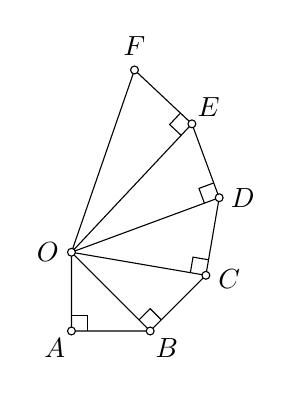
\begin{tikzpicture}
			\path
			(0,0) coordinate (A)
			(1,0) coordinate (B)
			(0,1) coordinate (O)
			($(B)!1cm!-90:(O)$) coordinate (C)
			($(C)!1cm!-90:(O)$) coordinate (D)
			($(D)!1cm!-90:(O)$) coordinate (E)
			($(E)!1cm!-90:(O)$) coordinate (F);
			\draw
			(O)--(A)--(B)--(C)--(D)--(E)--(F)--cycle (O)--(B) (O)--(C) (O)--(D) (O)--(E)
			pic[draw, angle radius=2mm]{right angle=O--A--B}
			pic[draw, angle radius=2mm]{right angle=O--B--C}
			pic[draw, angle radius=2mm]{right angle=O--C--D}
			pic[draw, angle radius=2mm]{right angle=O--D--E}
			pic[draw, angle radius=2mm]{right angle=O--E--F};
			\foreach \x/\g in {A/-135,B/-45,O/180,C/-10,D/0,E/45,F/90} \draw[fill=white] (\x) circle (.05) + (\g:.3) node{$\x$};
		\end{tikzpicture}
	\end{center}
	với $OA = AB = BC = CD = DE = EF = 1$ {\rm cm}. (a) Tính độ dài 5 đoạn t hẳng $OB,OC,OD,OE,OF$. (b) Vẽ đoạn thẳng có độ dài $\sqrt{10}$ {\rm cm}. (c) Nêu cách vẽ đoạn thẳng có độ dài $\sqrt{n}$ {\rm cm} với $n\in\mathbb{N}$ bằng thước thẳng \& compa.
\end{baitoan}

\begin{baitoan}[\cite{Binh_boi_duong_Toan_9_tap_1}, 1.14., p. 13]
	Tìm $n\in\mathbb{N}$ sao cho $\sqrt{4n + 1}\in\mathbb{N}$.
\end{baitoan}

\begin{baitoan}[\cite{Binh_boi_duong_Toan_9_tap_1}, 1.15., p. 13]
	Cho $A = \sqrt{2 + \sqrt{2 + \cdots + \sqrt{2}}}$ gồm $2015$ dấu căn bậc 2. Chứng minh $A\notin\mathbb{N}$.
\end{baitoan}

\begin{baitoan}[\cite{Binh_boi_duong_Toan_9_tap_1}, p. 14]
	Chứng minh đồng nhất thức: $\left(\dfrac{1}{a} + \dfrac{1}{b} + \dfrac{1}{c}\right)^2 = \dfrac{1}{a^2} + \dfrac{1}{b^2} + \dfrac{1}{c^2} + \dfrac{2(a + b + c)}{abc}$, $\forall a,b,c\in\mathbb{R}^\star$.
\end{baitoan}

\begin{baitoan}[\cite{Binh_boi_duong_Toan_9_tap_1}, p. 14]
	Chứng minh: $\sqrt{\dfrac{1}{a^2} + \dfrac{1}{b^2} + \dfrac{1}{c^2}} = \left|\dfrac{1}{a} + \dfrac{1}{b} + \dfrac{1}{c}\right|$, $\forall a,b,c\in\mathbb{R}^\star$ sao cho $a + b + c = 0$.
\end{baitoan}

\begin{baitoan}[\cite{Binh_boi_duong_Toan_9_tap_1}, p. 14]
	Chứng minh: $\sqrt{\dfrac{1}{a^2} + \dfrac{1}{b^2} + \dfrac{1}{(a + b)^2}} = \left|\dfrac{1}{a} + \dfrac{1}{b} - \dfrac{1}{a + b}\right|$, $\forall a,b\in\mathbb{R}^\star$, $a\ne-b$.
\end{baitoan}

\begin{baitoan}[\cite{Binh_boi_duong_Toan_9_tap_1}, p. 14]
	Chứng minh: $\sqrt{a^2 + \dfrac{1}{b^2} + \dfrac{a^2}{(ab + 1)^2}} = \left|a + \dfrac{1}{b} - \dfrac{a}{ab + 1}\right|$, $\forall a,b\in\mathbb{R}$, $b\ne0$, $ab\ne-1$.
\end{baitoan}

\begin{baitoan}[\cite{Binh_boi_duong_Toan_9_tap_1}, p. 14]
	Chứng minh: $\sqrt{a^2 + b^2 + \dfrac{a^2b^2}{(a + b)^2}} = \left|a + b - \dfrac{ab}{a + b}\right|$, $\forall a,b\in\mathbb{R}$, $a\ne-b$.
\end{baitoan}

\begin{baitoan}[\cite{Binh_boi_duong_Toan_9_tap_1}, 1., p. 14]
	Chứng minh với $a,b,c\in\mathbb{R}$ đôi một khác nhau: $\sqrt{\dfrac{1}{(a - b)^2} + \dfrac{1}{(b - c)^2} + \dfrac{1}{(c - a)^2}} = \left|\dfrac{1}{a - b} + \dfrac{1}{b - c} + \dfrac{1}{c - a}\right|$.
\end{baitoan}

\begin{baitoan}[\cite{Binh_boi_duong_Toan_9_tap_1}, 2., p. 15]
	Đơn giản biểu thức $A = \sqrt{\dfrac{1}{a^2 + b^2} + \dfrac{1}{(a + b)^2} + \sqrt{\dfrac{1}{a^4} + \dfrac{1}{b^4} + \dfrac{1}{(a^2 + b^2)^2}}}$, $\forall a,b\in\mathbb{R}^\star$, $a\ne-b$.
\end{baitoan}

\begin{baitoan}[\cite{Binh_boi_duong_Toan_9_tap_1}, 3., p. 15]
	Tính $A = \sqrt{1 + 2015^2 + \dfrac{2015^2}{2016^2}} + \dfrac{2015}{2016}$.
\end{baitoan}

\begin{baitoan}[\cite{Binh_boi_duong_Toan_9_tap_1}, 4., p. 15]
	Tính $A = \sqrt{0.43^2 + 0.57^2 + 0.43^2\cdot0.57^2}$.
\end{baitoan}

\begin{baitoan}
	Tính $A = \sqrt{x^2 + (1 - x)^2 + x^2\cdot(1 - x)^2}$, $\forall x\in\mathbb{R}$.
\end{baitoan}

\begin{baitoan}[\cite{Binh_boi_duong_Toan_9_tap_1}, p. 15]
	(a) Tính $A = \sum_{i=2}^{2015} \sqrt{1 + \dfrac{1}{i^2} + \dfrac{1}{(i + 1)^2}} = \sqrt{1 + \dfrac{1}{2^2} + \dfrac{1}{3^2}} + \sqrt{1 + \dfrac{1}{3^2} + \dfrac{1}{4^2}} + \cdots + \sqrt{1 + \dfrac{1}{2015^2} + \dfrac{1}{2016^2}}$. (b) Tính $A_n = \sum_{i=2}^n \sqrt{1 + \dfrac{1}{i^2} + \dfrac{1}{(i + 1)^2}} = \sqrt{1 + \dfrac{1}{2^2} + \dfrac{1}{3^2}} + \sqrt{1 + \dfrac{1}{3^2} + \dfrac{1}{4^2}} + \cdots + \sqrt{1 + \dfrac{1}{n^2} + \dfrac{1}{(n + 1)^2}}$, $\forall n\in\mathbb{N}^\star$.
\end{baitoan}

\begin{baitoan}[\cite{Binh_boi_duong_Toan_9_tap_1}, p. 15]
	(a) Tính $A = \sqrt{1 + \overline{\underbrace{99\ldots9}_{2015}}^2 + \overline{0.\underbrace{99\ldots9}_{2015}}^2}$. (b) Tính $A_n = \sqrt{1 + \overline{\underbrace{99\ldots9}_n}^2 + \overline{0.\underbrace{99\ldots9}_n}^2}$, $\forall n\in\mathbb{N}^\star$.
\end{baitoan}

%------------------------------------------------------------------------------%

\begin{baitoan}[\cite{Binh_Toan_9_tap_1}, Ví dụ 5, p. 7]
	Cho biểu thức $A = \sqrt{x - \sqrt{x^2 - 4x + 4}}$. (a) Tìm điều kiện xác định của biểu thức $A$. (b) Rút gọn biểu thức $A$.
\end{baitoan}

\begin{baitoan}[\cite{Binh_Toan_9_tap_1}, Ví dụ 6, p. 8]
	Tìm điều kiện xác định của các biểu thức: (a) $A = \dfrac{1}{\sqrt{x^2 - 2x - 1}}$. (b) $B = \dfrac{1}{\sqrt{x - \sqrt{2x + 1}}}$.
\end{baitoan}

\begin{baitoan}[\cite{Binh_Toan_9_tap_1}, Ví dụ 7, p. 8]
	Tìm các giá trị của $x$ sao cho $\sqrt{x + 1} < x + 3$.
\end{baitoan}

\begin{baitoan}[\cite{Binh_Toan_9_tap_1}, 7., p. 9]
	Tìm điều kiện xác định của các biểu thức: (a) $3 - \sqrt{1 - 16x^2}$. (b) $\dfrac{1}{1 - \sqrt{x^2 - 3}}$. (c) $\sqrt{8x - x^2 - 15}$. (d) $\dfrac{2}{\sqrt{x^2 - x + 1}}$. (e) $A = \dfrac{1}{\sqrt{x - \sqrt{2x - 1}}}$. (f) $B = \dfrac{\sqrt{16 - x^2}}{\sqrt{2x + 1}} + \sqrt{x^2 - 8x + 14}$.
\end{baitoan}

\begin{baitoan}[\cite{Binh_Toan_9_tap_1}, 8., p. 9]
	Cho biểu thức $A = \sqrt{x^2 - 6x + 9} - \sqrt{x^2 + 6x + 9}$. (a) Rút gọn biểu thức $A$. (b) Tìm các giá trị của $x$ để $A = 1$.
\end{baitoan}

\begin{baitoan}[\cite{Binh_Toan_9_tap_1}, 9., p. 9]
	Tìm các giá trị của $x$ sao cho: (a) $\sqrt{x^2 - 3}\le x^2 - 3$. (b) $\sqrt{x^2 - 6x + 9} > x - 6$.
\end{baitoan}

\begin{baitoan}[\cite{Binh_Toan_9_tap_1}, 10., p. 9]
	Cho $a + b + c = 0$ \& $abc\ne0$. Chứng minh hằng đẳng thức: $\sqrt{\dfrac{1}{a^2} + \dfrac{1}{b^2} + \dfrac{1}{c^2}} = \left|\dfrac{1}{a} + \dfrac{1}{b} + \dfrac{1}{c}\right|$.
\end{baitoan}

%------------------------------------------------------------------------------%

\section{Liên Hệ Giữa Phép Nhân, Phép Chia \& Phép Khai Phương}

\begin{baitoan}[\cite{Binh_boi_duong_Toan_9_tap_1}, p. 16]
	Với $A,B$ là 2 biểu thức đại số. Khi nào thì: $\sqrt{A + B} = \sqrt{A} + \sqrt{B}$. (b) $\sqrt{A - B} = \sqrt{A} - \sqrt{B}$?
\end{baitoan}

\begin{baitoan}[\cite{Binh_boi_duong_Toan_9_tap_1}, Ví dụ 1, p. 17]
	Tính: (a) $\sqrt{12.5\cdot10\cdot4500}$. (b) $\sqrt{685^2 - 684^2}$. (c) $\sqrt{\dfrac{27}{13}}:\sqrt{14\dfrac{10}{13}}$. (d) $\left(\sqrt{9 - \sqrt{17}} + \sqrt{9 + \sqrt{17}}\right)^2$.
\end{baitoan}

\begin{baitoan}[\cite{Binh_boi_duong_Toan_9_tap_1}, Ví dụ 2, p. 18]
	Tìm $x\in\mathbb{R}$ thỏa: (a) $\sqrt{8x}\cdot\sqrt{2} = 10$. (b) $\sqrt{x^2 - 9} - \sqrt{x + 3} = 0$. (c) $\dfrac{\sqrt{9x^2 - 25}}{\sqrt{3x - 5}} = 4$.
\end{baitoan}

\begin{baitoan}[\cite{Binh_boi_duong_Toan_9_tap_1}, Ví dụ 3, p. 18]
	2 bạn Việt \& Nam cùng giải bài toán tìm $x\in\mathbb{R}$: $\dfrac{\sqrt{2x - 5}}{\sqrt{x - 2}} = 2$. Việt làm như sau: $\dfrac{\sqrt{2x - 5}}{\sqrt{x - 2}} = 2\Leftrightarrow\sqrt{\dfrac{2x - 5}{x - 2}} = 2\Leftrightarrow\dfrac{2x - 5}{x - 2} = 4\Leftrightarrow2x - 5 = 4x - 8\Leftrightarrow2x = 3\Leftrightarrow x = 1.5$. Nam làm như sau: Điều kiện $2x - 5\ge0$ \& $x - 2> 0$, suy ra $x\ge2.5$. Rồi cũng giải để tìm ra $x = 1.5$ như Việt. Đối chiếu với điều kiện $x\ge2.5$, Nam kết luận phương trình vô nghiệm. Ai đúng ai sai? Giải thích.
\end{baitoan}

\begin{baitoan}[\cite{Binh_boi_duong_Toan_9_tap_1}, Ví dụ 4, p. 19]
	Rút gọn $(a + b)\sqrt{\dfrac{ab}{(a + b)^2}}$, $\forall a,b\in\mathbb{R}$, $a < 0$, $b < 0$.
\end{baitoan}

\begin{baitoan}[\cite{Binh_boi_duong_Toan_9_tap_1}, Ví dụ 5, p. 19]
	Rút gọn $A = \sqrt{2 + \sqrt{3}}\cdot \sqrt{2 + \sqrt{2 + \sqrt{3}}}\cdot\sqrt{2 + \sqrt{2 + \sqrt{2 + \sqrt{3}}}}\cdot\sqrt{2 - \sqrt{2 + \sqrt{2 + \sqrt{3}}}}$.
\end{baitoan}

\begin{baitoan}[\cite{Binh_boi_duong_Toan_9_tap_1}, Ví dụ 6, p. 19]
	Tính giá trị của biểu thức $A = \dfrac{x + 4 + 2\sqrt{16 - x^2}}{8 - 2x + \sqrt{16 - x^2}}$ tại $x = \dfrac{8}{\sqrt{3} + \frac{1}{\sqrt{3}}}$.
\end{baitoan}

\begin{baitoan}[\cite{Binh_boi_duong_Toan_9_tap_1}, Ví dụ 7, p. 20]
	(a) Cho $a\ge b\ge0$. Chứng minh: $\sqrt{a + b}\le\sqrt{a} + \sqrt{b}$, $\sqrt{a - b}\le\sqrt{a} - \sqrt{b}$. (b) Áp dụng: Tìm {\rm {\rm GTNN}} của $A = \sqrt{x - 5} + \sqrt{7 - x}$ \& {\rm GTLN} của $B = \sqrt{2x - 7} - \sqrt{2x - 11}$.
\end{baitoan}

\begin{luuy}
	Khi chứng minh bất đẳng thức chứa căn thức ta thường bình phương 2 vế \& sử dụng tính chất: Với $A\ge0$, $B\ge0$, $A^2 > B^2\Rightarrow A > B$, $A^2\ge B^2\Rightarrow A\ge B$.
\end{luuy}

\begin{baitoan}[\cite{Binh_boi_duong_Toan_9_tap_1}, 2.1., p. 20]
	Tính đường kính của 1 mặt ghế hình tròn, biết diện tích của nó bằng diện tích hình vuông có cạnh là {\rm2.6 dm}.
\end{baitoan}

\begin{baitoan}[\cite{Binh_boi_duong_Toan_9_tap_1}, 2.2., p. 20]
	Rút gọn $\left(\sqrt{xy} - 2\sqrt{\dfrac{y}{x}}\right)\sqrt{xy}$, $\forall x,y\in\mathbb{R}$, $x < 0$, $y < 0$.
\end{baitoan}

\begin{baitoan}[\cite{Binh_boi_duong_Toan_9_tap_1}, 2.3., p. 20]
	Tìm $x\in\mathbb{R}$ thỏa $\sqrt{4x^2 - 25} = \sqrt{4x + 10}$.
\end{baitoan}

\begin{baitoan}[\cite{Binh_boi_duong_Toan_9_tap_1}, 2.4., p. 20]
	Tính: (a)$\left(\dfrac{1}{2}\sqrt{\dfrac{1}{2}}\right):\left(\dfrac{4}{15}\sqrt{\dfrac{1}{8}}\right)$. (b) $\sqrt{27(1 - \sqrt{3})^2}:3\sqrt{75}$.
\end{baitoan}

\begin{baitoan}[\cite{Binh_boi_duong_Toan_9_tap_1}, 2.5., p. 21]
	So sánh: (a) $x = \sqrt{16} + \sqrt{28}$, $y = \sqrt{14} + \sqrt{30}$. (b) $x = \dfrac{\sqrt{319^2 - 306^2}}{\sqrt{67^2 - 54^2}}$, $y = \sqrt{23 - 8\sqrt{7}}(4 + \sqrt{7}):(3\sqrt{3})$.
\end{baitoan}

\begin{baitoan}[\cite{Binh_boi_duong_Toan_9_tap_1}, 2.6., p. 21]
	Tính: $A = \sqrt{2 + \sqrt{2}}\cdot\sqrt{3 + \sqrt{7 + \sqrt{2}}}\cdot\sqrt{3 + \sqrt{6 + \sqrt{7 + \sqrt{2}}}}\cdot\sqrt{3 - \sqrt{6 + \sqrt{7 + \sqrt{2}}}}$.
\end{baitoan}

\begin{baitoan}[\cite{Binh_boi_duong_Toan_9_tap_1}, 2.7., p. 21]
	Cho 6 số thực dương $a_1,b_1,c_1,a_2,b_2,c_2$ thoả mãn điều kiện $\dfrac{a_1}{a_2} = \dfrac{b_1}{b_2} = \dfrac{c_1}{c_2}$. Chứng minh:
	\begin{align*}
		\sqrt{(a_1 + b_1 + c_1)(a_2 + b_2 + c_2)} = \sqrt{a_1a_2} + \sqrt{b_1b_2} + \sqrt{c_1c_2}.
	\end{align*}
\end{baitoan}

\begin{baitoan}[\cite{Binh_boi_duong_Toan_9_tap_1}, 2.8., p. 21]
	Tìm {\rm GTLN}: (a) $A = \sqrt{3x - 5} - \sqrt{3x - 10}$. (b) $B = \sqrt{4x + 1} - \sqrt{16x - 12}$.
\end{baitoan}

\begin{baitoan}[\cite{Binh_boi_duong_Toan_9_tap_1}, 2.9., p. 21]
	Chứng minh: nếu 3 đoạn thẳng có độ dài $a,b,c\in\mathbb{R}$ lập thành 1 tam giác thì 3 đoạn thẳng có độ dài $\sqrt{a},\sqrt{b},\sqrt{c}$ cũng lập thành 1 tam giác.
\end{baitoan}

\begin{baitoan}[\cite{Binh_boi_duong_Toan_9_tap_1}, 2.10., p. 21]
	Cho $x = \sqrt{4 + \sqrt{10 + 2\sqrt{5}}} + \sqrt{4 - \sqrt{10 + 2\sqrt{5}}}$. (a) Chứng minh $x^2 - 2x = 4$. (b) Tính giá trị của biểu thức $f(x) = \dfrac{x^4 - 4x^3 - x^2 + 10x + 4}{x^3 - 3x + 5}$.
\end{baitoan}

\begin{baitoan}[\cite{Binh_boi_duong_Toan_9_tap_1}, p. 21, Vận tốc của máy thăm dò vũ trụ]
	Vận tốc tối thiểu của máy thăm dò vũ trụ để thắng sức hút của Trái Đất là $v = 1.15\cdot10^{-5}\sqrt{\dfrac{m}{r}}$, trong đó $m$ là khối lượng của Trái Đất tính theo {\rm kg}, $r$ là bán kính Trái Đất tính theo {\rm m}, $v$ là vận tốc máy thăm dò tính theo {\rm m{\tt/}s}. Biết $m\approx5.98\cdot10^{24}$ {\rm kg}, $r\approx6.38\cdot10^6$ {\rm m}. Tính vận tốc tối thiểu của máy thăm dò vũ trụ.
\end{baitoan}

\begin{dinhnghia}[Trung bình cộng, trung bình nhân, trung bình điều hòa]
	Cho $a,b\in\mathbb{R}$, $a,b > 0$. $m\coloneqq\dfrac{a + b}{2}$ được gọi là {\rm trung bình cộng} của $a,b$. $n\coloneqq\sqrt{ab}$ được gọi là {\rm trung bình nhân} của $a,b$. $p\coloneqq\dfrac{2}{\frac{1}{a} + \frac{1}{b}}$ được gọi là {\rm trung bình điều hòa} của $a,b$.
\end{dinhnghia}

\begin{baitoan}[\cite{Binh_boi_duong_Toan_9_tap_1}, p. 22]
	Cho $a,b\in\mathbb{R}$, $a,b > 0$. Gọi $m,n,p$ lần lượt là trung bình cộng, trung bình nhân, trung bình điều hòa của $a,b$. Chứng minh $p\le n\le m$. Đẳng thức xảy ra khi nào?
\end{baitoan}

\begin{baitoan}[\cite{Binh_boi_duong_Toan_9_tap_1}, p. 22]
	Vẽ $\Delta ABC$ vuông tại $A$, đường cao $AH$, trung tuyến $AM$ sao cho $BH = a$, $CH = b$. Hạ $HD\bot AM$ tại $D$. Chứng minh $AD\le AH\le AO$. Từ đó suy ra bất đẳng thức $p\le n\le m$ với $m,n,p$ lần lượt là trung bình cộng, trung bình nhân, trung bình điều hòa của $a,b$.
	\begin{center}
		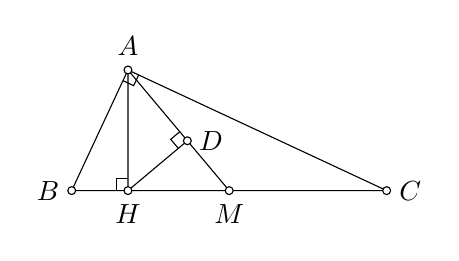
\begin{tikzpicture}
			\def\r{2}
			\path
			(130:\r) coordinate (A)
			(180:\r) coordinate (B)
			(0:\r) coordinate (C)
			($(B)!(A)!(C)$) coordinate (H)
			($(B)!.5!(C)$) coordinate (M)
			($(A)!(H)!(M)$) coordinate (D)
			;
			\draw
			(A)--(B)--(C)--cycle (A)--(H) (A)--(M) (H)--(D)
			pic[draw, angle radius=1.5mm]{right angle=B--A--C}
			pic[draw, angle radius=1.5mm]{right angle=A--H--B}
			pic[draw, angle radius=1.5mm]{right angle=A--D--H}			;
			\foreach \x/\g in {A/90,B/180,C/0,D/0,H/-90,M/-90} \draw[fill=white] (\x) circle (.05) + (\g:.3) node{$\x$};
		\end{tikzpicture}
	\end{center}
\end{baitoan}

\begin{dinhnghia}[Căn thức đồng dạng]
	2 căn thức bậc 2 được gọi là {\rm đồng dạng} nếu chúng có cùng biểu thức dưới dấu căn.
\end{dinhnghia}

\begin{vidu}[\cite{Binh_boi_duong_Toan_9_tap_1}, p. 22]
	(a) 3 biểu thức $\sqrt{7},2\sqrt{7},-5\sqrt{7}$ được gọi là {\rm đồng dạng} với nhau. (b) 3 biểu thức $\frac{1}{2}\sqrt{x},5\sqrt{x},-\frac{4}{7}\sqrt{x}$, $x\in\mathbb{R}$, $x\ge0$, được gọi là {\rm đồng dạng} với nhau.
\end{vidu}
Muốn cộng trừ các căn thức bậc 2 ta thu gọn các căn thức đồng dạng.

\begin{baitoan}[\cite{Binh_boi_duong_Toan_9_tap_1}, p. 23, Công thức căn phức tạp]
	Chứng minh:
	\begin{align}
		\label{can phuc tap}
		\sqrt{a\pm\sqrt{b}} = \sqrt{\frac{a + \sqrt{a^2 - b}}{2}}\pm\sqrt{\frac{a - \sqrt{a^2 - b}}{2}},\ \forall a,b\in\mathbb{R},\,a,b > 0,\,a^2\ge b.
	\end{align}
\end{baitoan}
Công thức \eqref{can phuc tap} được gọi là \textit{công thức căn phức tạp}. Nhờ công thức này, biểu thức $a\pm\sqrt{b}$ có thể dễ dàng viết được thành bình phương của 1 tổng hoặc hiệu, do đó tính được $a\pm\sqrt{b}$.

\begin{baitoan}[\cite{Binh_boi_duong_Toan_9_tap_1}, p. 23]
	Tính: (a) $A = 2\sqrt{3 + \sqrt{5 - \sqrt{13 + \sqrt{48}}}}$. (b) $B = \sqrt{4 + \sqrt{5\sqrt{3} + 5\sqrt{48 - 10\sqrt{7 + 4\sqrt{2}}}}}$.
\end{baitoan}

%------------------------------------------------------------------------------%

\section{Biến Đổi Đơn Giản Biểu Thức Chứa Căn Thức Bậc 2}
\cite[Chap. III, \S3, pp. 61--71]{SGK_Toan_9_Canh_Dieu_tap_1}: HD1. LT1. LT2. HD2. LT3. HD3. LT4. LT5. HD4. LT6. 1. 2. 3. 4. 5. 6. 7. 8. 9.

\begin{baitoan}[\cite{Binh_boi_duong_Toan_9_tap_1}, 1., p. 25]
	Đưa thừa số ra ngoài dấu căn của biểu thức $\sqrt{25(-a)^2b^3}$ với $b\ge0$.
\end{baitoan}

\begin{baitoan}[\cite{Binh_boi_duong_Toan_9_tap_1}, 2., p. 25]
	Đưa thừa số vào trong dấu căn của biểu thức $(1 - x)\sqrt{\dfrac{x}{x - 1}}$ với $x > 1$.
\end{baitoan}

\begin{baitoan}[\cite{Binh_boi_duong_Toan_9_tap_1}, 3--4., p. 21]
	(a) Khử mẫu của biểu thức $\sqrt{\dfrac{15}{24}}$. (b) Trục căn thức ở mẫu của biểu thức $\dfrac{2}{\sqrt{5} - \sqrt{3}}$.
\end{baitoan}

\begin{baitoan}[\cite{Binh_boi_duong_Toan_9_tap_1}, 5., p. 25]
	{\rm Đ{\tt/}S?} (a) $-3\sqrt{\dfrac{1}{2}} = \sqrt{(-3)^2\cdot\dfrac{1}{2}}$. (b) $\dfrac{3 - \sqrt{3}}{1 - \sqrt{3}} = \sqrt{3}$. (c) $-4\sqrt{3} < -3\sqrt{4}$. (d) $\dfrac{\sqrt{7} + 2}{\sqrt{7} - 2} = \dfrac{9 - 4\sqrt{7}}{3}$.
\end{baitoan}

\begin{baitoan}[\cite{Binh_boi_duong_Toan_9_tap_1}, Ví dụ 1, p. 25]
	Rút gọn biểu thức: (a) $A = \sqrt{12} + 3\sqrt{27} - 5\sqrt{48}$. (b) $B = 3\sqrt{a^2 + 2} - 3\sqrt{16a^2 + 32} + 4\sqrt{25a^2 + 50}$.
\end{baitoan}

\begin{baitoan}[\cite{Binh_boi_duong_Toan_9_tap_1}, Ví dụ 2, p. 26]
	Sắp xếp theo thứ tự tăng dần: $5\sqrt{2},\sqrt{39},3\sqrt{8},2\sqrt{15}$.
\end{baitoan}

\begin{baitoan}[\cite{Binh_boi_duong_Toan_9_tap_1}, Ví dụ 3, p. 26]
	Viết số nghịch đảo của mỗi số sau dưới dạng không chứa dấu căn ở mẫu: $4\sqrt{3},3\sqrt{5} + 5\sqrt{3},\dfrac{3 + \sqrt{3}}{3\sqrt{2}}$.
\end{baitoan}

\begin{baitoan}[\cite{Binh_boi_duong_Toan_9_tap_1}, p. 26]
	Chứng minh: $\dfrac{A}{a\sqrt{b} + c\sqrt{d}} = \dfrac{A(a\sqrt{b} - c\sqrt{d})}{a^2b - c^2d}$, $\forall A,a,b,c,d\in\mathbb{R}$, $b,d\ge0$, $a^2b\ne c^2d$.
\end{baitoan}

\begin{baitoan}[\cite{Binh_boi_duong_Toan_9_tap_1}, Ví dụ 4, p. 27]
	Tìm $x\in\mathbb{R}$ \& viết kết quả không chứa dấu căn ở mẫu: (a) $4(5 - x\sqrt{3}) + 6 = 10 - x\sqrt{12}$. (b) $x\sqrt{2} + \sqrt{5} = \sqrt{3}(1 + x) - \sqrt{20}$.
\end{baitoan}

\begin{baitoan}[\cite{Binh_boi_duong_Toan_9_tap_1}, Ví dụ 5, p. 27]
	Cho $x = \dfrac{\sqrt{3}}{\sqrt{\sqrt{3} - 1}} - \dfrac{\sqrt{3}}{\sqrt{\sqrt{3} + 1}}$. Tính $B = (x^4 - 2x^3 - x^2 + 2x - 1)^{2015}$.
\end{baitoan}

\begin{luuy}
	Căn thức liên hợp của $\sqrt{\sqrt{a} + b}\pm c$ là $\sqrt{\sqrt{a} + b}\mp c$.
\end{luuy}

\begin{baitoan}[\cite{Binh_boi_duong_Toan_9_tap_1}, Ví dụ 6, p. 27]
	Cho $A = \dfrac{x\sqrt{x} - 1}{x - \sqrt{x}} - \dfrac{x\sqrt{x} + 1}{x + \sqrt{x}} + \dfrac{x + 1}{\sqrt{x}}$. Tìm $x\in\mathbb{R}$ để $A = \dfrac{9}{2}$.
\end{baitoan}

\begin{baitoan}[\cite{Binh_boi_duong_Toan_9_tap_1}, Ví dụ 7, p. 28]
	Trục căn thức ở mẫu của biểu thức $\dfrac{1}{\sqrt{2} + \sqrt{3} - \sqrt{6}}$.
\end{baitoan}

\begin{luuy}
	Nếu mẫu số{\tt/}mẫu thức là tổng{\tt/}hiệu của $n$ căn thức với $n\in\mathbb{N}^\star$, $n\ge3$, ta phải thực hiện nhân biểu thức căn liên hợp khoảng $n - 1$ lần.
\end{luuy}

\begin{baitoan}[\cite{Binh_boi_duong_Toan_9_tap_1}, Ví dụ 8, p. 28]
	Tính $A = \dfrac{3 + \sqrt{5}}{2\sqrt{2} + \sqrt{3 + \sqrt{5}}} + \dfrac{3 - \sqrt{5}}{2\sqrt{2} - \sqrt{3 - \sqrt{5}}}$
\end{baitoan}

\begin{baitoan}[\cite{Binh_boi_duong_Toan_9_tap_1}, 3.1., p. 29]
	Sắp xếp theo thứ tự giảm dần: $3\sqrt{10},5\sqrt{3},\dfrac{20}{\sqrt{5}},12\sqrt{\dfrac{2}{3}}$.
\end{baitoan}

\begin{baitoan}[\cite{Binh_boi_duong_Toan_9_tap_1}, 3.2., p. 29]
	Rút gọn: (a) $\dfrac{2}{2a - 1}\sqrt{3a^2(4a^2 - 4a + 1)}$ với $0 < a < \dfrac{1}{2}$. (b) $\left(a\sqrt{\dfrac{10}{a}} + \sqrt{\dfrac{2a}{5}} + \sqrt{10a}\right):\sqrt{10a}$ với $a > 0$.
\end{baitoan}

\begin{baitoan}[\cite{Binh_boi_duong_Toan_9_tap_1}, 3.3., p. 29]
	Tìm $x\in\mathbb{R}$ thỏa: $\dfrac{2}{3}\sqrt{9x - 27} + \sqrt{x - 3} = 6 - \sqrt{4x - 12}$.
\end{baitoan}

\begin{baitoan}[\cite{Binh_boi_duong_Toan_9_tap_1}, 3.4., p. 29]
	Cho $x = \dfrac{\sqrt{5} + \sqrt{8}}{\sqrt{5} - \sqrt{8}}$. Tính $x + \dfrac{1}{x}$.
\end{baitoan}

\begin{baitoan}[\cite{Binh_boi_duong_Toan_9_tap_1}, 3.5., p. 29]
	Biết bình phương của 1 số bằng 3 lần số đó cộng với $1$. (a) Viết đẳng thức diễn tả mối quan hệ đó. (b) Chứng tỏ 2 số $\dfrac{3\pm\sqrt{13}}{2}$ là 2 số thỏa mãn bài toán.
\end{baitoan}

\begin{baitoan}[\cite{Binh_boi_duong_Toan_9_tap_1}, 3.6., p. 29]
	Tính $A = \dfrac{4 + \sqrt{7}}{3\sqrt{2} + \sqrt{4 + \sqrt{7}}} + \dfrac{4 - \sqrt{7}}{3\sqrt{2} - \sqrt{4 - \sqrt{7}}}$.
\end{baitoan}

\begin{baitoan}[\cite{Binh_boi_duong_Toan_9_tap_1}, 3.7., p. 29]
	Cho $A = (4x^5 + 4x^4 - 5x^3 + 2x - 2)^{2016} + 2015$. Tính giá trị của $A$ tại $x = \dfrac{-1 - \sqrt{5}}{2}$.
\end{baitoan}

\begin{baitoan}[\cite{Binh_boi_duong_Toan_9_tap_1}, 3.8., p. 29]
	Viết số nghịch đảo của mỗi số sau dưới dạng không chứa dấu căn ở mẫu: (a) $\sqrt{13 + 4\sqrt{3}}$. (b) $\sqrt{2} + \sqrt{3} - \sqrt{5}$.
\end{baitoan}

\begin{baitoan}[\cite{Binh_boi_duong_Toan_9_tap_1}, 3.9., p. 29]
	Rút gọn biểu thức $A = 2\sqrt{45\sqrt{3}} + 2\sqrt{20\sqrt{3}} - 3\sqrt{\sqrt{75}} - \sqrt{245\sqrt{3}}$.
\end{baitoan}

\begin{baitoan}[\cite{Binh_boi_duong_Toan_9_tap_1}, Ví dụ 1, p. 30]
	Tính tổng: (a) $S(2014) = \sum_{i=1}^{2014} \dfrac{1}{\sqrt{i} + \sqrt{i + 1}} = \dfrac{1}{1 + \sqrt{2}} + \dfrac{1}{\sqrt{2} + \sqrt{3}} + \cdots + \dfrac{1}{\sqrt{2014} + \sqrt{2015}}$. (b) $S(n) = \sum_{i=1}^n \dfrac{1}{\sqrt{i} + \sqrt{i + 1}} = \dfrac{1}{1 + \sqrt{2}} + \dfrac{1}{\sqrt{2} + \sqrt{3}} + \cdots + \dfrac{1}{\sqrt{n} + \sqrt{n + 1}}$, $\forall n\in\mathbb{N}^\star$.
\end{baitoan}

\begin{baitoan}[\cite{Binh_boi_duong_Toan_9_tap_1}, p. 30]
	Tính $S(n) = \sum_{i=1}^n \dfrac{1}{\sqrt{2i - 1} + \sqrt{2i + 1}} = \dfrac{1}{1 + \sqrt{3}} + \dfrac{1}{\sqrt{3} + \sqrt{5}} + \cdots + \dfrac{1}{\sqrt{2n - 1} + \sqrt{2n + 1}}$. Tính $S(1006)$.
\end{baitoan}

\begin{baitoan}[\cite{Binh_boi_duong_Toan_9_tap_1}, p. 30]
	Tính $S = \dfrac{1}{\sqrt{2} + \sqrt{6}} + \dfrac{1}{\sqrt{6} + \sqrt{10}} + \cdots + \dfrac{1}{\sqrt{2014} + \sqrt{2018}}$. Tìm công thức tổng quát.
\end{baitoan}

\begin{baitoan}[\cite{Binh_boi_duong_Toan_9_tap_1}, Ví dụ 2, p. 30]
	Tính tổng $S = \dfrac{1}{2\sqrt{1} + \sqrt{2}} + \dfrac{1}{3\sqrt{2} + 2\sqrt{3}} + \cdots + \dfrac{1}{2015\sqrt{2014} + 2014\sqrt{2015}}$. Tìm công thức tổng quát.
\end{baitoan}

\begin{baitoan}[\cite{Binh_boi_duong_Toan_9_tap_1}, Ví dụ 3, p. 31]
	Chứng minh $S = \dfrac{1}{2\sqrt{1}} + \dfrac{1}{3\sqrt{2}} + \cdots + \dfrac{1}{2016\sqrt{2015}} < 2$.
\end{baitoan}

\begin{luuy}
	Để tính tổng chứa căn thức có quy luật, ta thường biến đổi mỗi số hạng của tổng thành hiệu của 2 số có quy luật rồi giản ước liên tiếp chỉ còn lại số hạng đầu \& số hạng cuối. Tương tự, để ước lượng tổng chứa căn thức có quy luật, ta thường làm trội{\tt/}làm giảm mỗi số hạng của tổng bởi hiệu của 2 số có quy luật rồi giản ước liên tiếp chỉ còn lại số hạng đầu \& số hạng cuối.
\end{luuy}

%------------------------------------------------------------------------------%

\section{Rút Gọn Biểu Thức Có Chứa Căn Thức Bậc 2}
\cite[Chap. III, \S4, pp. 67--66]{SGK_Toan_9_Canh_Dieu_tap_1}: HD1. LT1. HD2. LT2. HD3. LT3. HD4. LT4. LT5. LT6. 1. 2. 3. 4. 5.

\begin{baitoan}[\cite{Binh_boi_duong_Toan_9_tap_1}, 1., p. 33]
	Tìm {\rm ĐKXĐ} của biểu thức $\dfrac{\sqrt{1 - 4x^2}}{1 + 2x}$.
\end{baitoan}

\begin{baitoan}[\cite{Binh_boi_duong_Toan_9_tap_1}, 2., p. 33]
	Rút gọn biểu thức $\sqrt{45(-x)^3y^4}:\sqrt{5(-x)y^2}$ với $x,y\in\mathbb{R}$, $x < 0$, $y\ne0$.
\end{baitoan}

\begin{baitoan}[\cite{Binh_boi_duong_Toan_9_tap_1}, 3., p. 33]
	Tính $(\sqrt{27} - 2\sqrt{3})\sqrt{7} - \sqrt{7}$.
\end{baitoan}

\begin{baitoan}[\cite{Binh_boi_duong_Toan_9_tap_1}, 4., p. 33]
	Rút gọn biểu thức $\dfrac{x\sqrt{y} - y\sqrt{x}}{\sqrt{xy}}:\dfrac{1}{\sqrt{x} + \sqrt{y}}$ với $x,y\in\mathbb{R}$, $x,y > 0$.
\end{baitoan}

\begin{baitoan}[\cite{Binh_boi_duong_Toan_9_tap_1}, Ví dụ 1, p. 33]
	Rút gọn biểu thức: (a) $\dfrac{(\sqrt{5} + 1)^3}{\sqrt{125} + 10}$. (b) $\dfrac{\sqrt{4 + \sqrt{15}}}{\sqrt{2}} - \dfrac{1}{\sqrt{3} - 1}$.
\end{baitoan}

\begin{baitoan}[\cite{Binh_boi_duong_Toan_9_tap_1}, Ví dụ 2, p. 34]
	Chứng minh đẳng thức: $\left(\dfrac{a\sqrt{a} - b\sqrt{b}}{\sqrt{a} - \sqrt{b}} + \sqrt{ab}\right)\cdot\left(\dfrac{\sqrt{a} - \sqrt{b}}{a - b}\right)^2 = 1$, $\forall a,b\in\mathbb{R}$, $a,b > 0$, $a\ne b$.
\end{baitoan}

\begin{baitoan}[\cite{Binh_boi_duong_Toan_9_tap_1}, Ví dụ 3, p. 34]
	Chứng minh biểu thức $A = \dfrac{-15\sqrt{a} + 3}{a + 2\sqrt{a} - 3} + \dfrac{5\sqrt{a} - 2}{\sqrt{a} - 1} - \dfrac{5\sqrt{a} + 3}{\sqrt{a} + 3}$ với $a\in\mathbb{R}$, $a\ge0$, $a\ne1$, không phụ thuộc vào biến $a$.
\end{baitoan}

\begin{baitoan}[\cite{Binh_boi_duong_Toan_9_tap_1}, Ví dụ 4, p. 34]
	Cho biểu thức $A = \left(\dfrac{x\sqrt{x} - 1}{x - \sqrt{x}} - \dfrac{x\sqrt{x} + 1}{x + \sqrt{x}}\right) + \left(\sqrt{x} - \dfrac{1}{\sqrt{x}}\right)\left(\dfrac{\sqrt{x} + 1}{\sqrt{x} - 1} + \dfrac{\sqrt{x} - 1}{\sqrt{x} + 1}\right)$ với $x\in\mathbb{R}$. (a) Tìm {\rm ĐKXĐ} rồi rút gọn biểu thức $A$. (b) Tìm giá trị của $A$ khi $x = 7 - 2\sqrt{6}$. (c) Tìm giá trị của $x$ để $A = \dfrac{62}{5}$. (d) Tìm {\rm {\rm GTNN}} của $A$.
\end{baitoan}

\begin{dinhly}[Nguyên tắc Dirichlet]
	Nếu đem nhốt $n + 1$ con chim bồ câu vào $n$ chiếc lồng thì tồn tại 1 lòng nhốt ít nhất $2$ con chim bồ câu.
\end{dinhly}

\begin{baitoan}[\cite{Binh_boi_duong_Toan_9_tap_1}, Ví dụ 5, p. 35]
	Cho tập hợp $Ã = \{\sqrt{1},\sqrt{2},\sqrt{3},\ldots,\sqrt{2015}\}$. Chứng minh trong $45$ số khác nhau tùy ý được lấy từ tập $A$ luôn tồn tại ít nhất 2 số có hiệu nhỏ hơn $1$.
\end{baitoan}

\begin{baitoan}[\cite{Binh_boi_duong_Toan_9_tap_1}, 4.1., p. 36]
	Tính: (a) $\left(a\sqrt{\dfrac{6}{a}} + \sqrt{\dfrac{2a}{3}} + \sqrt{6a}\right):\sqrt{6a}$, $\forall a\in\mathbb{R}$, $a > 0$. (b) $\dfrac{\sqrt{a}}{\sqrt{a} - \sqrt{b}} - \dfrac{\sqrt{b}}{\sqrt{a} + \sqrt{b}}$, $\forall a,b\in\mathbb{R}$, $a,b\ge0$, $a\ne b$.
\end{baitoan}

\begin{baitoan}[\cite{Binh_boi_duong_Toan_9_tap_1}, 4.2., p. 36]
	Chứng minh đẳng thức: (a) $\sqrt{23 + 8\sqrt{7}} - \sqrt{7} = 4$. (b) $\left(\dfrac{\sqrt{14} - \sqrt{7}}{1 - \sqrt{2}} + \dfrac{\sqrt{15} - \sqrt{5}}{1 - \sqrt{3}}\right):\dfrac{1}{\sqrt{7} - \sqrt{5}} = -2$.
\end{baitoan}

\begin{baitoan}[\cite{Binh_boi_duong_Toan_9_tap_1}, 4.3., p. 36]
	Cho hình vuông có độ dài cạnh bằng $1$. Chứng minh độ dài đường chéo của nó bằng $m = \dfrac{2 + \sqrt{3}}{\sqrt{2} + \sqrt{2 + \sqrt{3}}} + \dfrac{2 - \sqrt{3}}{\sqrt{2} - \sqrt{2 - \sqrt{3}}}$.
\end{baitoan}

\begin{baitoan}[\cite{Binh_boi_duong_Toan_9_tap_1}, 4.4., p. 36]
	Cho tam giác đều có độ dài cạnh bằng $1$. Chứng minh độ dài đường cao của nó bằng $h = \dfrac{\sqrt{2 + \sqrt{3}} + \sqrt{2 - \sqrt{3}}}{2\sqrt{2}}$.
\end{baitoan}

\begin{baitoan}[\cite{Binh_boi_duong_Toan_9_tap_1}, 4.5., p. 36]
	Cho biểu thức $A = \left(\dfrac{\sqrt{a} + 3}{\sqrt{a} + 2} + \dfrac{4a\sqrt{a} + 3a + 9}{a - \sqrt{a} - 6}\right):\left(\dfrac{\sqrt{a}}{\sqrt{a} + 3} + \dfrac{2\sqrt{a} + 3}{a + 5\sqrt{a} + 6}\right)$. (a) Tìm {\rm ĐKXĐ} rồi rút gọn $A$. (b) Tìm $a\in\mathbb{R}$ để $A = 48$.
\end{baitoan}

\begin{baitoan}[\cite{Binh_boi_duong_Toan_9_tap_1}, 4.6., p. 36]
	Cho biểu thức $A = \dfrac{x\sqrt{x} - 4x - \sqrt{x} + 4}{2x\sqrt{x} - 14x + 28\sqrt{x} - 16}$. (a) Tìm $x$ để $A$ có nghĩa. (b) Rút gọn $A$. (c) Tìm tất cả $x\in\mathbb{N}$ sao cho $A$ nhận giá trị nguyên.
\end{baitoan}

\begin{baitoan}[\cite{Binh_boi_duong_Toan_9_tap_1}, 4.7., p. 36]
	Số Fibonacci là số có dạng $F_n = \dfrac{1}{\sqrt{5}}\left[\left(\dfrac{1 + \sqrt{5}}{2}\right)^n - \left(\dfrac{1 - \sqrt{5}}{2}\right)^n\right]$, $\forall n\in\mathbb{N}$. (a) Tính $F_0,F_1,F_2,F_3$. (b) Chứng minh công thức truy hồi $F_{n + 2} = F_n + F_{n + 1}$, $\forall n\in\mathbb{N}$.
\end{baitoan}

\begin{baitoan}[\cite{Binh_boi_duong_Toan_9_tap_1}, 4.8., p. 36]
	Tìm $n\in\mathbb{N}$ nhỏ nhất sao cho: (a) $S(n) = \dfrac{1}{1 + \sqrt{2}} + \dfrac{1}{\sqrt{2} + \sqrt{3}} + \cdots + \dfrac{1}{\sqrt{n} + \sqrt{n + 1}}\ge2015$. (b) $S(n)\ge a$ với $a\in\mathbb{R}$ cho trước.
\end{baitoan}

\begin{baitoan}[\cite{Binh_boi_duong_Toan_9_tap_1}, 4.9., p. 36, Trò chơi toán học]
	Trên bảng viết 4 số $\sqrt{3} + 1,\sqrt{3} - 1,\sqrt{3},\dfrac{1}{\sqrt{3}}$. Ta thực hiện trò chơi như sau: Mỗi lần chơi, ta xóa 2 số nào đó trong 4 số trên (giả sử là $a,b$) rồi thay vào 2 số mới $\dfrac{a + b}{\sqrt{2}}$ \& $\dfrac{|a - b|}{\sqrt{2}}$ đồng thời giữa nguyên 2 số còn lại. Như vậy sau mỗi lần chơi trên bảng vẫn luôn có 4 số. Hỏi có bao giờ trên bảng có ghi 4 số $\dfrac{\sqrt{3}}{\sqrt{2}},\sqrt{3} + \sqrt{2},\sqrt{3} - \sqrt{2},3$ không?
\end{baitoan}

\begin{baitoan}[\cite{Binh_boi_duong_Toan_9_tap_1}, p. 36]
	Công thức của Heron để khai phương 1 số mà không dùng bảng số hoặc máy tính: $\sqrt{a^2 + b}\approx a + \dfrac{b}{2a}$. (a) Tìm điều kiện của $a,b\in\mathbb{R}$ để công thức này có nghĩa. (b) Tính sai số của công thức khai phương xấp xỉ của Heron. (c) Áp dụng công thức của Heron để xấp xỉ $\sqrt{85},\sqrt{154},\sqrt{99},\sqrt{2015}$.
\end{baitoan}

%------------------------------------------------------------------------------%

\section{Phương Trình Vô Tỷ}

\begin{dinhnghia}[Phương trình vô tỷ]
	{\rm Phương trình vô tỷ} là phương trình đại số chứa ẩn số trong biểu thức dưới dấu căn.
\end{dinhnghia}
2 dạng cơ bản của phương trình vô tỷ:
\begin{equation*}
	\boxed{\sqrt{f(x)} = g(x)\Leftrightarrow\left\{\begin{split}
		g(x)&\ge0,\\
		f(x) &= g^2(x),
	\end{split}\right.\ \sqrt{f(x)} = \sqrt{g(x)}\Leftrightarrow\left\{\begin{split}
	f(x)&\ge0,\\
	f(x) &= g(x),
	\end{split}\right.\Leftrightarrow\left\{\begin{split}
		g(x)&\ge0,\\
		f(x) &= g(x).
	\end{split}\right.}
\end{equation*}
Phương trình vô tỷ có nhiều cách giải, e.g., phương pháp nâng lên lũy thừa, phương pháp vận dụng căn liên hợp, phương pháp đưa về phương trình chứa dấu giá trị tuyệt đối, phương pháp sử dụng bất đẳng thức hoặc đánh giá 2 vế của phương trình.

\begin{baitoan}[\cite{Binh_boi_duong_Toan_9_tap_1}, Ví dụ 1, p. 38]
	Giải phương trình $\sqrt{x + 7} - 1 = x$.
\end{baitoan}

\begin{baitoan}[\cite{Binh_boi_duong_Toan_9_tap_1}, Ví dụ 2, p. 38]
	Giải phương trình $\sqrt{x + 1} + \sqrt{2x + 3} = \sqrt{3x} + \sqrt{2x - 2}$.
\end{baitoan}

\begin{baitoan}[\cite{Binh_boi_duong_Toan_9_tap_1}, Ví dụ 3, p. 38]
	Giải phương trình $\sqrt{6x + 5} + x = \sqrt{3x + 11} + 2$.
\end{baitoan}

\begin{baitoan}[\cite{Binh_boi_duong_Toan_9_tap_1}, Ví dụ 4, p. 39]
	Giải phương trình $\sqrt{x + 2\sqrt{x - 1}} + \sqrt{x - 2\sqrt{x - 1}} = 2$.
\end{baitoan}

\begin{baitoan}[\cite{Binh_boi_duong_Toan_9_tap_1}, Ví dụ 5, p. 39]
	Giải phương trình $\sqrt{2x - 3} + \sqrt{5 - 2x} = 3x^2 - 12x + 14$.
\end{baitoan}

\begin{baitoan}[\cite{Binh_boi_duong_Toan_9_tap_1}, p. 39]
	Giải phương trình $\sqrt{x - 4} + \sqrt{6 - x} = x^2 - 10x + 27$.
\end{baitoan}

\begin{baitoan}[\cite{Binh_boi_duong_Toan_9_tap_1}, p. 39]
	Giải phương trình $x + y + z - 2\sqrt{x} -2\sqrt{y + 1} - 2\sqrt{z - 1} + 3 = 0$.
\end{baitoan}

\begin{baitoan}[\cite{Binh_boi_duong_Toan_9_tap_1}, p. 39]
	Giải phương trình $\sqrt{4x + 7} + x = \sqrt{2x + 1} - 3$.
\end{baitoan}

\begin{baitoan}[\cite{Binh_boi_duong_Toan_9_tap_1}, p. 39]
	Giải phương trình $\sqrt{x + 2 + 3\sqrt{2x - 5}} + \sqrt{x - 2 - 3\sqrt{2x - 5}} = 2\sqrt{2}$.
\end{baitoan}

%------------------------------------------------------------------------------%

\section{Cube Root -- Căn Bậc 3}

\begin{baitoan}[\cite{Binh_boi_duong_Toan_9_tap_1}, 2., p. 41]
	Rút gọn biểu thức $\sqrt[3]{125} - \sqrt[3]{-27} - \sqrt[3]{512}$.
\end{baitoan}

\begin{baitoan}[\cite{Binh_boi_duong_Toan_9_tap_1}, 3., p. 41]
	Đưa thừa số vào trong dấu căn của biểu thức $(2 - x)^3 \sqrt{\dfrac{x}{x - 2}}$.
\end{baitoan}

\begin{baitoan}[\cite{Binh_boi_duong_Toan_9_tap_1}, 4., p. 41]
	Khử căn thức ở mẫu của $\sqrt[3]{\dfrac{5}{12}}$.
\end{baitoan}

\begin{baitoan}[\cite{Binh_boi_duong_Toan_9_tap_1}, 5., p. 41]
	Trục căn thức ở mẫu của $\dfrac{2}{1 + \sqrt[3]{2}}$.
\end{baitoan}

\begin{baitoan}[\cite{Binh_boi_duong_Toan_9_tap_1}, Ví dụ 1, p. 41]
	Tính cạnh của hình lập phương, biết thể tích của nó bằng thể tích của hình hộp chữ nhật có 3 kích thước là {\rm4.8 m, 3 m, 15 m}.
\end{baitoan}

\begin{baitoan}[\cite{Binh_boi_duong_Toan_9_tap_1}, Ví dụ 2, p. 42]
	Tính: (a) $\sqrt[3]{\sqrt{10} + \sqrt{2}}\cdot\sqrt[3]{\sqrt{2} - \sqrt{10}}$. (b) $\dfrac{\sqrt[3]{-54}}{\sqrt[3]{16}}$. (c) $\sqrt[3]{128} + \sqrt[3]{-250} - 7\sqrt[3]{16}$. (d) $\sqrt[3]{8x^8y^5} - 4xy\sqrt[3]{x^5y^2}$.
\end{baitoan}

\begin{baitoan}[\cite{Binh_boi_duong_Toan_9_tap_1}, Ví dụ 3, p. 42]
	So sánh: (a) $5\sqrt[3]{6}$ \& $6\sqrt[3]{5}$. (b) $\sqrt[3]{-7}:\sqrt[3]{49}$ \& $-8$.
\end{baitoan}

\begin{baitoan}[\cite{Binh_boi_duong_Toan_9_tap_1}, Ví dụ 4, p. 43]
	Tìm $x\in\mathbb{R}$ thỏa: (a) $\sqrt[3]{2x + 1} = 5$. (b) $\sqrt[3]{x + 1} - 1 = x$.
\end{baitoan}

\begin{baitoan}[\cite{Binh_boi_duong_Toan_9_tap_1}, Ví dụ 5, p. 43]
	Cho $A = \sqrt[3]{20 + 14\sqrt{2}} + \sqrt[3]{20 - 14\sqrt{2}}$. Tính giá trị của biểu thức $A^3 - 6A$.
\end{baitoan}

\begin{baitoan}[\cite{Binh_boi_duong_Toan_9_tap_1}, Ví dụ 6, p. 43]
	Cho biểu thức $A = \dfrac{8 - x}{2 + \sqrt[3]{x}}:\left(2 + \dfrac{\sqrt[3]{x^2}}{2 + \sqrt[3]{x}}\right) + \left(\sqrt[3]{x} + \dfrac{2\sqrt[3]{x}}{\sqrt[3]{x} - 2}\right)\cdot\dfrac{\sqrt[3]{x^2} - 4}{\sqrt[3]{x^2} + 2\sqrt[3]{x}}$. (a) Tìm {\rm ĐKXĐ}. (b) Chứng minh giá trị của $B$ không phụ thuộc vào $x$.
\end{baitoan}

\begin{baitoan}[\cite{Binh_boi_duong_Toan_9_tap_1}, 5.1., p. 44]
	Tính: (a) $(\sqrt[3]{9} + \sqrt[3]{6} + \sqrt[3]{4})(\sqrt[3]{3} - \sqrt[3]{2})$. (b) $\sqrt[3]{38 + 17\sqrt{5}}$. (c) $\sqrt{\sqrt[3]{729}}$,
\end{baitoan}

\begin{baitoan}[\cite{Binh_boi_duong_Toan_9_tap_1}, 5.2., p. 44]
	So sánh: (a) $5$ \& $\sqrt[3]{130}$. (b) $\sqrt{122 - 22\sqrt{2}} + \sqrt[3]{77\sqrt{2} - 155}$ \& $6$.
\end{baitoan}

\begin{baitoan}[\cite{Binh_boi_duong_Toan_9_tap_1}, 5.3., p. 44]
	Tìm $x\in\mathbb{R}$ thỏa: (a) $\sqrt[3]{x + 1} = -5$. (b) $\sqrt[3]{x + 3} - x = 3$.
\end{baitoan}

\begin{baitoan}[\cite{Binh_boi_duong_Toan_9_tap_1}, 5.4., p. 44]
	Trục căn thức ở mẫu: (a) $\dfrac{1}{\sqrt[3]{2} + \sqrt[3]{3}}$. (b) $\dfrac{1}{\sqrt[3]{9} + \sqrt[3]{6} + \sqrt[3]{4}}$.
\end{baitoan}

\begin{baitoan}[\cite{Binh_boi_duong_Toan_9_tap_1}, 5.5., p. 44]
	Cho $a = \sqrt[3]{7 + 5\sqrt{2}} - \dfrac{1}{\sqrt[3]{7 + 5\sqrt{2}}}$. Tính $a^3 + 3a$.
\end{baitoan}

\begin{baitoan}[\cite{Binh_boi_duong_Toan_9_tap_1}, 5.6., p. 44]
	Chứng minh $b = \sqrt[3]{1 + \dfrac{\sqrt{84}}{9}} + \sqrt[3]{1 - \dfrac{\sqrt{84}}{9}}$ là 1 số nguyên.
\end{baitoan}

\begin{baitoan}[\cite{Binh_boi_duong_Toan_9_tap_1}, 5.7., p. 44]
	Cho $ax^3 = by^3 = cz^3$ \& $\dfrac{1}{x} + \dfrac{1}{y} + \dfrac{1}{z} = 1$. Chứng minh $\sqrt[3]{ax^2 + by^2 + cz^2} = \sqrt[3]{a} + \sqrt[3]{b} + \sqrt[3]{c}$.
\end{baitoan}

\begin{baitoan}[\cite{Binh_boi_duong_Toan_9_tap_1}, 5.8., p. 44]
	Cho $x = \dfrac{2}{2\sqrt[3]{2} + 2 + \sqrt[3]{4}}$ \& $y = \dfrac{6}{2\sqrt[3]{2} - 2 + \sqrt[3]{4}}$. Tính giá trị của $T = xy^3 - x^3y$.
\end{baitoan}

%------------------------------------------------------------------------------%

\section{$n$th Root -- Căn Bậc $n$}

\begin{baitoan}[\cite{Binh_boi_duong_Toan_9_tap_1}, Ví dụ 1, p. 46]
	So sánh $3\sqrt[4]{3}$ \& $4\sqrt{2}$.
\end{baitoan}

\begin{baitoan}[\cite{Binh_boi_duong_Toan_9_tap_1}, Ví dụ 2, p. 46]
	Chứng minh $\sqrt[4]{\dfrac{3 + 2\sqrt[4]{5}}{3 - 2\sqrt[4]{5}}} = \dfrac{\sqrt[4]{5} + 1}{\sqrt[4]{5} - 1}$.
\end{baitoan}

\section{Liên Hệ Giữa Phép Nhân, Phép Chia \& Phép Khai Phương}

\begin{baitoan}[\cite{SGK_Toan_9_tap_1}, ?1, p. 12]
	Tính \& so sánh: $\sqrt{16\cdot25}$ \& $\sqrt{16}\cdot\sqrt{25}$.	
\end{baitoan}

\begin{baitoan}[\cite{SGK_Toan_9_tap_1}, ĐL, p. 12]
	Chứng minh: (a) $\sqrt{ab} = \sqrt{a}\sqrt{b}$, $\forall a,b\in\mathbb{R}$, $a,b\ge0$. (b)
	\begin{align*}
		\sqrt{\prod_{i=1}^n a_i} = \prod_{i=1}^n \sqrt{a_i},\mbox{ i.e., }\sqrt{a_1a_2\cdots a_n} = \sqrt{a_1}\sqrt{a_2}\cdots\sqrt{a_n},\ \forall n\in\mathbb{N}^\star,\ \forall a_i\in\mathbb{R},\,a_i\ge0,\,\forall i = 1,2,\ldots,n.
	\end{align*}
\end{baitoan}

\begin{baitoan}[\cite{SGK_Toan_9_tap_1}, Ví dụ 1, ?2, p. 13]
	Áp dụng quy tắc khai phương 1 tích, tính: (a) $\sqrt{49\cdot1.44\cdot25}$. (b) $\sqrt{810\cdot40}$. (c) $\sqrt{0.16\cdot0.64\cdot225}$. (d) $\sqrt{250\cdot360}$.
\end{baitoan}

\begin{baitoan}[\cite{SGK_Toan_9_tap_1}, Ví dụ 2, ?3, pp. 13--14]
	Tính: (a) $\sqrt{5}\sqrt{20}$. (b) $\sqrt{1.3}\sqrt{52}\sqrt{10}$. (c) $\sqrt{3}\sqrt{75}$. (d) $\sqrt{20}\sqrt{72}\sqrt{4.9}$.
\end{baitoan}

\begin{baitoan}[\cite{SGK_Toan_9_tap_1}, Ví dụ 3, ?4, p. 14]
	Tìm ĐKXĐ rồi rút gọn biểu thức: (a) $\sqrt{3a}\sqrt{27a}$ với $a\ge0$. (b) $\sqrt{9a^2b^4}$. (c) $\sqrt{3a^3}\sqrt{12a}$. (d) $\sqrt{2a\cdot32ab^2}$.
\end{baitoan}

\begin{baitoan}[\cite{SGK_Toan_9_tap_1}, 17., p. 14]
	Áp dụng quy tắc khai phương 1 tích, tính: (a) $\sqrt{0.09\cdot64}$. (b) $\sqrt{2^4\dot(-7)^2}$. (c) $\sqrt{12.1\cdot360}$. (d) $\sqrt{2^2\cdot3^4}$.
\end{baitoan}

\begin{baitoan}[\cite{SGK_Toan_9_tap_1}, 18., p. 14]
	Áp dụng quy tắc nhân các căn bậc 2, tính: (a) $\sqrt{7}\sqrt{63}$. (b) $\sqrt{2.5}\sqrt{30}\sqrt{48}$. (c) $\sqrt{0.4}\cdot\sqrt{6.4}$. (d) $\sqrt{2.7}\sqrt{5}\sqrt{1.5}$.
\end{baitoan}

\begin{baitoan}[\cite{SGK_Toan_9_tap_1}, 19., p. 15]
	Rút gọn biểu thức: (a) $\sqrt{0.36a^2}$ với $a < 0$ \& $a\in\mathbb{R}$. (b) $\sqrt{a^4(3 - a)^2}$ với $a\ge3$ \& $a\in\mathbb{R}$. (c) $\sqrt{27\cdot48(1 - a)^2}$ với $a > 1$ \& $a\in\mathbb{R}$. (d) $\frac{1}{a - b}\sqrt{a^4(a - b)^2}$ với $a > b$.
\end{baitoan}

\begin{baitoan}[\cite{SGK_Toan_9_tap_1}, 20., p. 15]
	Rút gọn biểu thức: (a) $\sqrt{\frac{2a}{3}}\sqrt{\frac{3a}{8}}$ với $a\ge0$. (b) $\sqrt{13a}\sqrt{\frac{52}{a}}$ với $a > 0$. (c) $\sqrt{5a}\sqrt{45a} - 3a$ với $a\ge0$. (d) $(3 - a)^2 - \sqrt{0.2}\sqrt{180a^2}$.
\end{baitoan}

\begin{baitoan}[\cite{SGK_Toan_9_tap_1}, 21., p. 15]
	Khai phương tích $12\cdot30\cdot40$ được bao nhiêu?
\end{baitoan}

\begin{baitoan}[\cite{SGK_Toan_9_tap_1}, 22., p. 15]
	Tính hợp lý: (a) $\sqrt{13^2 - 12^2}$. (b) $\sqrt{17^2 - 8^2}$. (c) $\sqrt{117^2 - 108^2}$. (d) $\sqrt{313^2 - 312^2}$.
\end{baitoan}

\begin{baitoan}[Mở rộng \cite{SGK_Toan_9_tap_1}, 22., p. 15]
	Rút gọn biểu thức:
	\begin{align*}
		\sqrt{\left(\frac{m^2 + n^2}{2}\right)^2 - \left(\frac{m^2 - n^2}{2}\right)^2},\ \forall m,n\in\mathbb{R}.
	\end{align*}
\end{baitoan}

\begin{baitoan}[\cite{SGK_Toan_9_tap_1}, 23., p. 15]
	Chứng minh: (a) $(2 - \sqrt{3})(2 + \sqrt{3}) = 1$. (b) $\sqrt{2006}\pm\sqrt{2005})$ là 2 số nghịch đảo của nhau.
\end{baitoan}

\begin{baitoan}[Mở rộng \cite{SGK_Toan_9_tap_1}, 23., p. 15]
	Chứng minh: (a) $(n - \sqrt{n^2 - 1})(n + \sqrt{n^2 - 1}) = 1$, $\forall n\in\mathbb{R}$, $|n|\ge1$. (b) $\sqrt{n + 1}\pm\sqrt{n})$ là 2 số nghịch đảo của nhau, $\forall n\in\mathbb{R}$, $n\ge0$.
\end{baitoan}

\begin{baitoan}[\cite{SGK_Toan_9_tap_1}, 24., p. 15]
	Rút gọn \& tìm giá trị (làm tròn đến chữ số thập phân thứ 3) của các căn thức: (a) $\sqrt{4(1 + 6x + 9x^2)^2}$ tại $x = -\sqrt{2}$. (b) $\sqrt{9a^2(b^2 + 4 - 4b)}$ tại $a = -2$, $b = -\sqrt{3}$. 
\end{baitoan}

\begin{baitoan}[\cite{SGK_Toan_9_tap_1}, 25., p. 16]
	Tìm $x\in\mathbb{R}$ thỏa: (a) $\sqrt{16x} = 8$. (b) $\sqrt{4x} = \sqrt{5}$. (c) $\sqrt{9(x - 1)} = 21$. (d) $\sqrt{4(1 - x)^2} - 6 = 0$.
\end{baitoan}

\begin{baitoan}[\cite{SGK_Toan_9_tap_1}, 26., p. 16]
	(a) So sánh $\sqrt{25 + 9}$ \& $\sqrt{25} + \sqrt{9}$. (b) Chứng minh $\sqrt{a + b} < \sqrt{a} + \sqrt{b}$, $\forall a,b\in\mathbb{R}$, $a,b > 0$. (c) Chứng minh $\sqrt{a + b}\le\sqrt{a} + \sqrt{b}$, $\forall a,b\in\mathbb{R}$, $a,b\ge0$.
\end{baitoan}

\begin{baitoan}[\cite{SGK_Toan_9_tap_1}, 27., p. 16]
	So sánh: (a) $4$ \& $2\sqrt{3}$. (b) $-\sqrt{5}$ \& $-2$.
\end{baitoan}

\begin{baitoan}[\cite{SBT_Toan_9_tap_1}, 23., p. 9]
	Tính: (a) $\sqrt{10}\sqrt{40}$. (b) $\sqrt{5}\sqrt{45}$. (c) $\sqrt{52}\sqrt{13}$. (d) $\sqrt{2}\sqrt{162}$.
\end{baitoan}

\begin{baitoan}[\cite{SBT_Toan_9_tap_1}, 24., p. 9]
	Tính: (a) $\sqrt{45\cdot80}$. (b) $\sqrt{75\cdot48}$. (c) $\sqrt{90\cdot6.4}$. (d) $\sqrt{2.5\cdot14.4}$.
\end{baitoan}

\begin{baitoan}[\cite{SBT_Toan_9_tap_1}, 25., p. 9]
	Rút gọn rồi tính: (a) $\sqrt{6.8^2 - 3.2^2}$. (b) $\sqrt{21.8^2 - 18.2^2}$. (c) $\sqrt{117.5^2 - 26.5^2 - 1440}$.  (d) $\sqrt{146.5^2 - 109.5^2 + 27.256}$.
\end{baitoan}

\begin{baitoan}[\cite{SBT_Toan_9_tap_1}, 26., p. 9]
	Chứng minh: (a) $\sqrt{9 - \sqrt{17}}\sqrt{9 + \sqrt{17}} = 8$. (b) $2\sqrt{2}(\sqrt{3} - 2) + (1 + 2\sqrt{2})^2 - 2\sqrt{6} = 9$.
\end{baitoan}

\begin{baitoan}[\cite{SBT_Toan_9_tap_1}, 27., p. 9]
	Rút gọn: (a) $\dfrac{\sqrt{6} + \sqrt{14}}{2\sqrt{3} + \sqrt{28}}$. (b) $\dfrac{\sqrt{2} + \sqrt{3} + \sqrt{6} + \sqrt{8} + \sqrt{16}}{\sqrt{2} + \sqrt{3} + \sqrt{4}}$.
\end{baitoan}

\begin{baitoan}[\cite{SBT_Toan_9_tap_1}, 28., p. 9]
	Không dùng bảng số hay máy tính bỏ túi, so sánh: (a) $\sqrt{2} + \sqrt{3}$ \& $\sqrt{10}$. (b) $\sqrt{3} + 2$ \& $\sqrt{2} + \sqrt{6}$. (c) $16$ \& $\sqrt{15}\sqrt{17}$. (d) $8$ \& $\sqrt{15} + \sqrt{17}$.
\end{baitoan}

\begin{baitoan}[\cite{SBT_Toan_9_tap_1}, 29., p. 9]
	Không dùng bảng số hay máy tính bỏ túi, so sánh: (a) $\sqrt{2003} + \sqrt{2005}$ \& $2\sqrt{2004}$.
\end{baitoan}

\begin{baitoan}[\cite{SBT_Toan_9_tap_1}, 30., p. 9]
	Cho 2 biểu thức $A = \sqrt{x + 2}\sqrt{x - 3}$, $B = \sqrt{(x + 2)(x - 3)}$. (a) Tìm $x\in\mathbb{R}$ lần lượt để $A,B$  có nghĩa. (b) Với giá trị nào của $x$ thì $A = B$?
\end{baitoan}

\begin{baitoan}[\cite{SBT_Toan_9_tap_1}, 31., p. 10]
	Biểu diễn $\sqrt{ab}$ ở dạng tích các căn bậc 2 với $a < 0$ \& $b < 0$. Áp dụng tính $\sqrt{(-25)\cdot(-64)}$.
\end{baitoan}

\begin{baitoan}[\cite{SBT_Toan_9_tap_1}, 32., p. 10]
	Rút gọn các biểu thức: (a) $\sqrt{4(a - 3)^2}$ với $a\ge3$ \& $a\in\mathbb{R}$. (b) $\sqrt{9(b - 2)^2}$ với $b < 2$ \& $b\in\mathbb{R}$. (c) $\sqrt{a^2(a + 1)^2}$ với $a > 0$ \& $a\in\mathbb{R}$. (d) $\sqrt{b^2(b - 1)^2}$ với $b < 0$ \& $b\in\mathbb{R}$.
\end{baitoan}

\begin{baitoan}[\cite{SBT_Toan_9_tap_1}, 33., p. 10]
	(a) Tìm ĐKXĐ \& biến đổi các biểu thức sau về dạng tích: $A(x) = \sqrt{x^2 - 4} + 2\sqrt{x - 2}$, $B(x) = 3\sqrt{x + 3} + \sqrt{x^2 - 9}$. (b) Giải phương trình $A(x) = 0$ \& $B(x) = 0$.
\end{baitoan}

\begin{baitoan}[\cite{SBT_Toan_9_tap_1}, 34., p. 10]
	Tìm $x\in\mathbb{R}$ thỏa: (a) $\sqrt{x - 5} = 3$. (b) $\sqrt{x - 10} = -2$. (c) $\sqrt{2x - 1} = \sqrt{5}$. (d) $\sqrt{4 - 5x} = 12$.
\end{baitoan}

\begin{baitoan}[\cite{SBT_Toan_9_tap_1}, 35., p. 10]
	(a) Chứng minh: $\left(\sqrt{n + 1} - \sqrt{n}\right)^2 = \sqrt{(2n + 1)^2} - \sqrt{(2n + 1)^2 - 1}$, $\forall n\in\mathbb{N}$. Viết đẳng thức trên khi $n = 1,2,3,4$. (B) Đẳng thức trên còn đúng khi $n\in\mathbb{Z}$ \& $n\in\mathbb{R}$ không?
\end{baitoan}

\begin{baitoan}[\cite{SGK_Toan_9_tap_1}, ?1, p. 16]
	Tính \& so sánh: $\sqrt{\dfrac{16}{25}}$ \& $\dfrac{\sqrt{16}}{\sqrt{25}}$.
\end{baitoan}

\begin{baitoan}[\cite{SGK_Toan_9_tap_1}, ĐL, p. 16]
	Chứng minh: $\sqrt{\dfrac{a}{b}} = \dfrac{\sqrt{a}}{\sqrt{b}}$, $\forall a,b\in\mathbb{R}$, $a\ge0$, $b > 0$.
\end{baitoan}

\begin{baitoan}[\cite{SGK_Toan_9_tap_1}, Ví dụ 1, ?2, p. 17]
	Áp dụng quy tắc khai phương 1 thương, tính: (a) $\sqrt{\dfrac{25}{121}}$. (b) $\sqrt{\dfrac{9}{16}:\dfrac{25}{36}}$. (a) $\sqrt{\dfrac{225}{256}}$. (d) $\sqrt{0.0196}$.
\end{baitoan}

\begin{baitoan}[\cite{SGK_Toan_9_tap_1}, Ví dụ 2, ?3, pp. 17--18]
	Tính: (a) $\dfrac{\sqrt{80}}{\sqrt{5}}$. (b) $\sqrt{\dfrac{49}{8}}:\sqrt{3\dfrac{1}{8}}$. (c) $\dfrac{\sqrt{999}}{\sqrt{111}}$. (d) $\dfrac{\sqrt{52}}{\sqrt{117}}$.
\end{baitoan}

\begin{baitoan}[\cite{SGK_Toan_9_tap_1}, Ví dụ 3, ?4, p. 18]
	Rút gọn biểu thức: (a) $\sqrt{\dfrac{4a^2}{25}}$. (b) $\dfrac{\sqrt{27a}}{\sqrt{3a}}$ với $a > 0$. (c) $\sqrt{\dfrac{2a^2b^4}{50}}$. (d) $\dfrac{\sqrt{2ab^2}}{\sqrt{162}}$ với $a\ge0$.
\end{baitoan}

\begin{baitoan}[\cite{SGK_Toan_9_tap_1}, 28., p. 18]
	Tính: (a) $\sqrt{\dfrac{289}{225}}$. (b) $\sqrt{2\dfrac{14}{25}}$. (c) $\sqrt{\dfrac{0.25}{9}}$. (d) $\sqrt{\dfrac{8.1}{1.6}}$.
\end{baitoan}

\begin{baitoan}[\cite{SGK_Toan_9_tap_1}, 29., p. 19]
	Tính: (a) $\dfrac{\sqrt{2}}{\sqrt{18}}$. (b) $\dfrac{\sqrt{15}}{\sqrt{735}}$. (c) $\dfrac{\sqrt{12500}}{\sqrt{500}}$. (d) $\dfrac{\sqrt{6^5}}{\sqrt{2^3\cdot3^5}}$.
\end{baitoan}

\begin{baitoan}[\cite{SGK_Toan_9_tap_1}, 30., p. 19]
	Rút gọn biểu thức: (a) $\dfrac{y}{x}\sqrt{\dfrac{x^2}{y^4}}$ với $x > 0$ \& $y\ne0$. (b) $2y^2\sqrt{\dfrac{x^4}{4y^2}}$ với $y < 0$. (c) $5xy\sqrt{\dfrac{25x^2}{y^6}}$ với $x < 0$, $y > 0$. (d) $0.2x^3y^3\sqrt{\dfrac{16}{x^4y^8}}$ với $xy\ne0$.
\end{baitoan}

\begin{baitoan}[\cite{SGK_Toan_9_tap_1}, 31., p. 19]
	(a) So sánh $\sqrt{25 - 16}$ \& $\sqrt{25} - \sqrt{16}$. (b) Chứng minh: $\sqrt{a} - \sqrt{b} < \sqrt{a - b}$, $\forall a,b\in\mathbb{R}$, $a > b > 0$.
\end{baitoan}

\begin{baitoan}[\cite{SGK_Toan_9_tap_1}, 32., p. 19]
	Tính: (a) $\sqrt{1\dfrac{9}{16}\cdot5\dfrac{4}{9}\cdot0.01}$. (b) $\sqrt{1.44\cdot1.21 - 1.44\cdot0.4}$. (c) $\sqrt{\dfrac{165^2 - 124^2}{164}}$. (d) $\sqrt{\dfrac{149^2 - 76^2}{457^2 - 384^2}}$.
\end{baitoan}

\begin{baitoan}[\cite{SGK_Toan_9_tap_1}, 33., p. 19]
	Giải phương trình: (a)  $\sqrt{2}x - \sqrt{50} = 0$. (b) $\sqrt{3}x + \sqrt{3} = \sqrt{12} + \sqrt{27}$. (c) $\sqrt{3}x^2 - \sqrt{12} = 0$. (d) $\dfrac{x^2}{\sqrt{5}} - \sqrt{20} = 0$.
\end{baitoan}

\begin{baitoan}[\cite{SGK_Toan_9_tap_1}, 34., pp. 19--20]
	Rút gọn biểu thức: (a) $ab^2\sqrt{\dfrac{3}{a^2b^4}}$ với $a < b$, $b\ne0$. (b) $\sqrt{\dfrac{27(a - 3)^2}{48}}$ với $a > 3$. (c) $\sqrt{\dfrac{9 + 12a + 4a^2}{b^2}}$ với $a\ge-1.5$ \& $b < 0$. (d) $(a - b)\sqrt{\dfrac{ab}{(a - b)^2}}$ với $a < b < 0$.
\end{baitoan}

\begin{baitoan}[\cite{SGK_Toan_9_tap_1}, 35., p. 20]
	Tìm $x\in\mathbb{R}$ thỏa: (a) $\sqrt{(x - 3)^2} = 9$. (b) $\sqrt{4x^2 + 4x + 1} = 6$.
\end{baitoan}

\begin{baitoan}[\cite{SGK_Toan_9_tap_1}, 36., p. 20]
	\emph{Đ\texttt{/}S?} (a) $0.01 = \sqrt{0.0001}$. (b) $-0.5 = \sqrt{-0.25}$. (c) $6 < \sqrt{39} < 7$. (d) $(4 - \sqrt{13})2x < \sqrt{3}(4 - \sqrt{13})\Leftrightarrow2x < \sqrt{3}$.
\end{baitoan}

\begin{baitoan}[\cite{SBT_Toan_9_tap_1}, 36., p. 10]
	Áp dụng quy tắc khai phương 1 thương, tính: (a) $\sqrt{\dfrac{9}{169}}$. (b) $\sqrt{\dfrac{25}{144}}$. (c) $\sqrt{1\dfrac{9}{16}}$. (d) $\sqrt{2\dfrac{7}{81}}$.
\end{baitoan}

\begin{baitoan}[\cite{SBT_Toan_9_tap_1}, 37., p. 11]
	Áp dụng quy tắc chia căn bậc 2, tính: (a) $\dfrac{\sqrt{2300}}{\sqrt{23}}$. (b) $\dfrac{\sqrt{12.5}}{\sqrt{0.5}}$. (c) $\dfrac{\sqrt{192}}{\sqrt{12}}$. (d) $\dfrac{\sqrt{6}}{\sqrt{150}}$.
\end{baitoan}

\begin{baitoan}[\cite{SBT_Toan_9_tap_1}, 38., p. 11]
	Cho các biểu thức $A = \sqrt{\dfrac{2x + 3}{x - 3}}$, $B = \dfrac{\sqrt{2x + 3}}{\sqrt{x - 3}}$. (a) Tìm $x\in\mathbb{R}$ lần lượt để $A,B$ có nghĩa. (b) Với giá trị nào của $x\in\mathbb{R}$ thì $A = B$?
\end{baitoan}

\begin{baitoan}[\cite{SBT_Toan_9_tap_1}, 39., p. 11]
	Biểu diễn $\sqrt{\dfrac{a}{b}}$ với $a,b < 0$ ở dạng thương của 2 căn thức. Áp dụng tính $\sqrt{\dfrac{-49}{-81}}$.
\end{baitoan}

\begin{baitoan}[\cite{SBT_Toan_9_tap_1}, 40., p. 11]
	Rút gọn biểu thức: (a) $\dfrac{\sqrt{63y^3}}{\sqrt{7y}}$, $y > 0$. (b) $\dfrac{\sqrt{48x^3}}{\sqrt{3x^5}}$, $x > 0$. (c) $\dfrac{\sqrt{45mn^2}}{\sqrt{20m}}$, $m,n > 0$. (d) $\dfrac{\sqrt{16a^4b^6}}{\sqrt{128a^6b^6}}$, $a < 0$, $b\ne0$.
\end{baitoan}

\begin{baitoan}[\cite{SBT_Toan_9_tap_1}, 41., pp. 11--12]
	Rút gọn biểu thức: (a) $\sqrt{\dfrac{x - 2\sqrt{x} + 1}{x + 2\sqrt{x} + 1}}$, $x\ge0$. (b) $\dfrac{x - 1}{\sqrt{y} - 1}\sqrt{\dfrac{y - 2\sqrt{y} + 1}{(x - 1)^4}}$, $x\ne1$, $y\ne1$, $y\ge0$.
\end{baitoan}

\begin{baitoan}[\cite{SBT_Toan_9_tap_1}, 42., p. 12]
	Rút gọn biểu thức với điều kiện đã cho của $x$ rồi tính giá trị của nó: (a) $\sqrt{\dfrac{(x - 2)^4}{(3 - x)^2}} + \dfrac{x^2 - 1}{x - 3}$, $x < 3$, tại $x = 0.5$. (b) $4x - \sqrt{8} + \dfrac{\sqrt{x^3 + 2x^2}}{\sqrt{x + 2}}$, $x > -2$, tại $x = -\sqrt{2}$.
\end{baitoan}

\begin{baitoan}[\cite{SBT_Toan_9_tap_1}, 43., p. 12]
	Tìm $x\in\mathbb{R}$ thỏa: (a) $\sqrt{\dfrac{2x - 3}{x - 1}} = 2$. (b) $\dfrac{\sqrt{2x - 3}}{\sqrt{x - 1}} = 2$. (c) $\sqrt{\dfrac{4x + 3}{x + 1}} = 3$. (d) $\dfrac{\sqrt{4x + 3}}{\sqrt{x + 1}} = 3$.
\end{baitoan}

\begin{baitoan}[\cite{SBT_Toan_9_tap_1}, 44., p. 12]
	Chứng minh bất đẳng thức Cauchy cho 2 số không âm:
	\begin{align*}
		\frac{a + b}{2}\ge\sqrt{ab},\ \forall a,b\in\mathbb{R},\,a,b\ge0.
	\end{align*}
	Dấu đẳng thức xảy ra khi nào?
\end{baitoan}

\begin{baitoan}[\cite{SBT_Toan_9_tap_1}, 45., p. 12]
	Chứng minh:
	\begin{align*}
		\sqrt{\frac{a + b}{2}}\ge\frac{\sqrt{a} + \sqrt{b}}{2},\ \forall a,b\in\mathbb{R},\,a,b\ge0.
	\end{align*}
\end{baitoan}

\begin{baitoan}[\cite{SBT_Toan_9_tap_1}, 46., p. 12]
	Chứng minh: $a + \frac{1}{a}\ge2$, $\forall a\in\mathbb{R}$, $a > 0$.
\end{baitoan}

\begin{baitoan}[\cite{SBT_Toan_9_tap_1}, 52., p. 13]
	Chứng $\sqrt{2}$ là số vô tỷ.
\end{baitoan}

\begin{baitoan}[\cite{SBT_Toan_9_tap_1}, 53., p. 13]
	Chứng minh: (a) $\sqrt{3}$ là số vô tỷ. (b) $5\sqrt{2},3 + \sqrt{2}$ đều là số vô tỷ.
\end{baitoan}

\begin{baitoan}[\cite{SBT_Toan_9_tap_1}, 54., p. 14]
	Tìm tập hợp các số thực $x$ thỏa mãn bất đẳng thức $\sqrt{x} > 2$ \& biểu diễn tập hợp đó trên trục số.
\end{baitoan}

\begin{baitoan}[\cite{SBT_Toan_9_tap_1}, 55., p. 14]
	Tìm tập hợp các số thực $x$ thỏa mãn bất đẳng thức $\sqrt{x} < 3$ \& biểu diễn tập hợp đó trên trục số.
\end{baitoan}

\begin{baitoan}[\cite{Tuyen_Toan_9_old}, Thí dụ 3, p. 9]
	Rút gọn biểu thức $A = \sqrt{4 + \sqrt{7}} - \sqrt{4 - \sqrt{7}}$.
\end{baitoan}

\begin{baitoan}[\cite{Tuyen_Toan_9_old}, Thí dụ 4, p. 10]
	Tìm giá trị lớn nhất của biểu thức $A = \sqrt{x - 5} + \sqrt{13 - x}$.
\end{baitoan}

\begin{baitoan}[\cite{Tuyen_Toan_9_old}, 14., p. 11]
	Rút gọn biểu thức $A = \dfrac{\sqrt{\sqrt{7} - \sqrt{3}} - \sqrt{\sqrt{7} + \sqrt{3}}}{\sqrt{\sqrt{7} - 2}}$.
\end{baitoan}

\begin{baitoan}[\cite{Tuyen_Toan_9_old}, 15., p. 11]
	Cho 2 số có tổng bằng $\sqrt{19}$ \& có hiệu bằng $\sqrt{7}$. Tính tích của 2 số đó.
\end{baitoan}

\begin{baitoan}[\cite{Tuyen_Toan_9_old}, 16., p. 11]
	Tính $\sqrt{A}$ biết: (a) $A = 13 - 2\sqrt{42}$. (b) $A = 46 + 6\sqrt{5}$. (c) $A = 12 - 3\sqrt{15}$.
\end{baitoan}

\begin{baitoan}[\cite{Tuyen_Toan_9_old}, 17., p. 12]
	Rút gọn biểu thức: (a) $A = \sqrt{6 + 2\sqrt{2}\sqrt{3 - \sqrt{4 + 2\sqrt{3}}}}$. (b) $B = \sqrt{5} - \sqrt{3 - \sqrt{29 - 12\sqrt{5}}}$. (c) $C = \sqrt{3 - \sqrt{5}}(\sqrt{10} - \sqrt{2})(3 + \sqrt{5})$.
\end{baitoan}

\begin{baitoan}[\cite{Tuyen_Toan_9_old}, 18., p. 12]
	Rút gọn biểu thức $A = \sqrt{x + 2\sqrt{x - 1}} + \sqrt{x - 2\sqrt{x - 1}}$.
\end{baitoan}

\begin{baitoan}[\cite{Tuyen_Toan_9_old}, 19., p. 12]
	Cho $a > 0$, so sánh $\sqrt{a + 1} + \sqrt{a + 3}$ với $2\sqrt{a + 2}$.
\end{baitoan}

\begin{baitoan}[\cite{Tuyen_Toan_9_old}, 20., p. 12]
	Cho $a,b,x,y > 0$. Chứng minh $\sqrt{ax} + \sqrt{by}\le\sqrt{(a + b)(x + y)}$.
\end{baitoan}

\begin{baitoan}[\cite{Tuyen_Toan_9_old}, 21., p. 12]
	(a) Tìm giá trị lớn nhất của biểu thức $A = \sqrt{x + 1} - \sqrt{x - 8}$. (b) Tìm giá trị nhỏ nhất của biểu thức $B = \sqrt{x - 1} + \sqrt{5 - x}$.
\end{baitoan}

\begin{baitoan}[\cite{Tuyen_Toan_9_old}, 22., p. 12]
	Rút gọn biểu thức:
	\begin{align*}
		A = \frac{\sqrt{1 + \sqrt{1 - x^2}}\left[\sqrt{(1 + x)^3} - \sqrt{(1 - x)^3}\right]}{2 + \sqrt{1 - x^2}}.
	\end{align*}
\end{baitoan}

\begin{baitoan}[\cite{Tuyen_Toan_9_old}, 23., p. 12]
	Tìm $x,y$ biết $x + y + 12 = 4\sqrt{x} + 6\sqrt{y - 1}$.
\end{baitoan}

\begin{baitoan}[\cite{Tuyen_Toan_9_old}, 24., p. 12]
	Tìm $x,y,z$ biết $\sqrt{x - a} + \sqrt{y - b} + \sqrt{z - c} = \frac{1}{2}(x + y + z)$, trong đó $a + b + c = 3$.
\end{baitoan}

\begin{baitoan}[\cite{Tuyen_Toan_9_old}, 25., p. 12]
	Giải phương trình $\sqrt{x + 3 - 4\sqrt{x - 1}} + \sqrt{x + 8 + 6\sqrt{x - 1}} = 5$.
\end{baitoan}

\begin{baitoan}[\cite{Tuyen_Toan_9_old}, 26., p. 12]
	Giải phương trình $\sqrt{x^2 - 5x + 6} + \sqrt{x + 1} = \sqrt{x - 2} + \sqrt{x^2 - 2x - 3}$.
\end{baitoan}

\begin{baitoan}[\cite{Tuyen_Toan_9_old}, 27., p. 12]
	Chứng minh bất đẳng thức $\sqrt{n + a} + \sqrt{n - a} < 2\sqrt{n}$ vpwos $0 < |a|\le n$. Áp dụng (không dùng máy tính hoặc bảng số): Chứng minh: $\sqrt{101} - \sqrt{99} > 0.1$.
\end{baitoan}

\begin{baitoan}[\cite{Tuyen_Toan_9_old}, 28., p. 13]
	Chứng minh: $2(\sqrt{n + 1} - \sqrt{n}) < \dfrac{1}{\sqrt{n}} < 2(\sqrt{n} - \sqrt{n - 1})$, $\forall n\in\mathbb{N}^\star$. Áp dụng: Cho $S = \sum_{i=1}^{100} \frac{1}{\sqrt{i}} = 1 + \frac{1}{\sqrt{2}} + \frac{1}{\sqrt{3}} + \cdots + \frac{1}{\sqrt{100}}$. Chứng minh $18 < S < 19$.
\end{baitoan}

\begin{baitoan}[\cite{Tuyen_Toan_9_old}, 29., p. 13]
	Chứng minh: $\dfrac{1}{2\sqrt{n + 1}} < \sqrt{n + 1} - \sqrt{n}$, $\forall n\in\mathbb{N}^\star$. Áp dụng: Chứng minh: $S = \sum_{i=1}^{2500} \frac{1}{\sqrt{i}} = 1 + \frac{1}{\sqrt{2}} + \frac{1}{\sqrt{3}} + \cdots + \frac{1}{\sqrt{2500}} < 100$.
\end{baitoan}

\begin{baitoan}[\cite{Tuyen_Toan_9_old}, 30., p. 13]
	Cho $x,y,z > 0$. Chứng minh $x + y + z\ge\sqrt{xy} + \sqrt{yz} + \sqrt{zx}$.
\end{baitoan}

\begin{baitoan}[\cite{Tuyen_Toan_9_old}, 31., p. 13]
	Cho $A = \sqrt{x + 3} + \sqrt{5 - x}$. Chứng minh $A\le4$.
\end{baitoan}

\begin{baitoan}[\cite{Tuyen_Toan_9_old}, 32., p. 13]
	Cho $B = \dfrac{x^3}{1 + y} + \dfrac{y^3}{1 + x}$ trong đó $x,y$ là các số thực dương thỏa mãn điều kiện $xy = 1$. Chứng minh $B\ge1$.
\end{baitoan}

\begin{baitoan}[\cite{Tuyen_Toan_9_old}, 33., p. 13]
	Cho $x,y,z > 0$ thỏa mãn điều kiện $\dfrac{1}{x + 1} + \dfrac{1}{y + 1} + \dfrac{1}{z + 1} = 2$. Chứng minh $xyz\le\frac{1}{8}$.
\end{baitoan}

\begin{baitoan}[\cite{Tuyen_Toan_9_old}, 34., p. 13]
	Tìm các số dương $x,y,z$ sao cho $x + y + z = 3$ \& $x^4 + y^4 + z^4 = 3xyz$.
\end{baitoan}

\begin{baitoan}[\cite{Tuyen_Toan_9_old}, 35., p. 13]
	Cho $\sqrt{x} + 2\sqrt{y} = 10$. Chứng minh: $x + y\ge20$.
\end{baitoan}

\begin{baitoan}[\cite{Tuyen_Toan_9_old}, 36., p. 13]
	Cho $x,y,z\ge0$ thỏa mãn điều kiện $x + y + z = 1$. Chứng minh: $\sqrt{x + y} + \sqrt{y + z} + \sqrt{z + x}\le\sqrt{6}$.
\end{baitoan}

\begin{baitoan}[\cite{Binh_Toan_9_tap_1}, Ví dụ 8, p. 10]
	Rút gọn biểu thức $A = \sqrt{x + \sqrt{2x - 1}} - \sqrt{ x - \sqrt{2x - 1}}$.
\end{baitoan}

\begin{baitoan}[\cite{Binh_Toan_9_tap_1}, Ví dụ 9, p. 11]
	Chứng minh số $\sqrt{2} + \sqrt{3} + \sqrt{5}$ là số vô tỷ.
\end{baitoan}

\begin{baitoan}[\cite{Binh_Toan_9_tap_1}, 11., pp. 11--12]
	Rút gọn biểu thức: (a) $\sqrt{11 - 2\sqrt{10}}$. (b) $\sqrt{9 - 2\sqrt{14}}$. (c) $\sqrt{4 + 2\sqrt{3}} - \sqrt{4 - 2\sqrt{3}}$. (d) $\sqrt{9 - 4\sqrt{5}} - \sqrt{9 + 4\sqrt{5}}$. (e) $\sqrt{4 - \sqrt{7}} - \sqrt{4 + \sqrt{7}}$. (f) $\dfrac{\sqrt{3} + \sqrt{11 + 6\sqrt{2}}- \sqrt{5 + 2\sqrt{6}}}{\sqrt{2} + \sqrt{6 + 2\sqrt{5}} - \sqrt{7 + 2\sqrt{10}}}$. (g) $\sqrt{5\sqrt{3} + 5\sqrt{48 - 10\sqrt{7+ 4\sqrt{3}}}}$. (h) $\sqrt{4 + \sqrt{10 + 2\sqrt{5}}} + \sqrt{4 - \sqrt{10 + 2\sqrt{5}}}$. (i) $\sqrt{94 - 42\sqrt{5}} - \sqrt{94 + 42\sqrt{5}}$.
\end{baitoan}

\begin{baitoan}[\cite{Binh_Toan_9_tap_1}, 12., p. 12]
	Tính: (a) $(4 + \sqrt{15})(\sqrt{10} - \sqrt{6})\sqrt{4 - \sqrt{15}}$. (b) $\sqrt{3 - \sqrt{5}}(\sqrt{10} - \sqrt{2})(3 + \sqrt{5})$.\\(c) $\dfrac{\sqrt{\sqrt{5} + 2} + \sqrt{\sqrt{5} - 2}}{\sqrt{\sqrt{5} + 1}} - \sqrt{3 - 2\sqrt{2}}$.
\end{baitoan}

\begin{baitoan}[\cite{Binh_Toan_9_tap_1}, 13., p. 12]
	Chứng minh các hằng đẳng thức sau với $b\ge0$, $a\ge\sqrt{b}$: (a) $\sqrt{a + \sqrt{b}}\pm\sqrt{a - \sqrt{b}} = \sqrt{2(a\pm\sqrt{a^2 - b})}$. (b) $\sqrt{a\pm\sqrt{b}} = \sqrt{\dfrac{a + \sqrt{a^2 - b}}{2}}\pm\sqrt{\dfrac{a - \sqrt{a^2 - b}}{2}}$.
\end{baitoan}

\begin{baitoan}[\cite{Binh_Toan_9_tap_1}, 14., p. 12]
	Rút gọn biểu thức $A = \sqrt{x + 2\sqrt{2x - 4}} + \sqrt{x - 2\sqrt{2x - 4}}$.
\end{baitoan}

\begin{baitoan}[\cite{Binh_Toan_9_tap_1}, 15., p. 12]
	Cho biểu thức $A = \dfrac{x + \sqrt{x^2 - 2x}}{x - \sqrt{x^2 - 2x}} - \dfrac{x - \sqrt{x^2 - 2x}}{x + \sqrt{x^2 - 2x}}$. (a) Tìm điều kiện xác định của biểu thức $A$. (b) Rút gọn biểu thức $A$. (c) Tìm giá trị của $x$ để $A < 2$.
\end{baitoan}

\begin{baitoan}[\cite{Binh_Toan_9_tap_1}, 16., p. 12]
	Lập 1 phương trình bậc 2 với các hệ số nguyên, trong đó: (a) $2 + \sqrt{3}$ là 1 nghiệm của phương trình. (b) $6 - 4\sqrt{2}$ là 1 nghiệm của phương trình.
\end{baitoan}

\begin{baitoan}[\cite{Binh_Toan_9_tap_1}, 17., p. 13]
	Chứng minh các số sau là số vô tỷ: (a) $\sqrt{3} - \sqrt{2}$. (b) $2\sqrt{2} + \sqrt{3}$.
\end{baitoan}

\begin{baitoan}[\cite{Binh_Toan_9_tap_1}, 18., p. 13]
	Có tồn tại các số hữu tỷ dương $a,b$ hay không nếu: (a) $\sqrt{a} + \sqrt{b} = \sqrt{2}$. (b) $\sqrt{a} + \sqrt{b} = \sqrt{\sqrt{2}}$.
\end{baitoan}

\begin{baitoan}[\cite{Binh_Toan_9_tap_1}, 19., p. 13]
	Cho 3 số $x,y,\sqrt{x} + \sqrt{y}$ là các số hữu tỷ. Chứng minh mỗi số $\sqrt{x},\sqrt{y}$ đều là số hữu tỷ.
\end{baitoan}

\begin{baitoan}[\cite{Binh_Toan_9_tap_1}, 20., p. 13]
	Cho $a,b,c,d$ là các số dương. Chứng minh tồn tại 1 số dương trong 2 số $2a + b - 2\sqrt{cd}$ \& $2c + d - 2\sqrt{ab}$.
\end{baitoan}

\begin{baitoan}[\cite{Binh_Toan_9_tap_1}, $21^\star$., p. 13]
	(a) Rút gọn biểu thức $A = \sqrt{1 + \dfrac{1}{a^2} + \dfrac{1}{(a + 1)^2}}$ với $a > 0$. (b) Tính giá trị của tổng $B = \sum_{i=1}^{99} \sqrt{1 + \dfrac{1}{i^2} + \dfrac{1}{(i + 1)^2}} = \sqrt{1 + \dfrac{1}{1^2} + \frac{1}{2^2}} + \sqrt{1 + \dfrac{1}{2^2} + \dfrac{1}{3^2}} + \sqrt{1 + \dfrac{1}{3^2} + \dfrac{1}{4^2}} + \cdots + \sqrt{1 + \dfrac{1}{99^2} + \dfrac{1}{100^2}}$.
\end{baitoan}

\begin{baitoan}[\cite{Binh_Toan_9_tap_1}, $22^\star$., p. 13]
	(a) Nêu 1 cách tính nhẩm $997^2$. (b) Tính tổng các chữ số của $A$ biết $\sqrt{A} = 99\ldots96$ (có $100$ chữ số $9$).
\end{baitoan}

%------------------------------------------------------------------------------%

\section{Biến Đổi Đơn Giản Biểu Thức Chứa Căn Thức Bậc 2}

\begin{baitoan}[\cite{SGK_Toan_9_tap_1}, ?1, p. 24]
	Chứng minh: $\sqrt{a^2b} = a\sqrt{b}$, $\forall a,b\in\mathbb{R}$, $a,b\ge0$.
\end{baitoan}

\begin{baitoan}[\cite{SGK_Toan_9_tap_1}, Ví dụ 1--2, ?2, pp. 24--25]
	Rút gọn: (a) $\sqrt{2\cdot3^2}$. (b) $\sqrt{20}$. (c) $3\sqrt{5} + \sqrt{20} + \sqrt{5}$. (d) $\sqrt{2} + \sqrt{8} + \sqrt{50}$. (e) $4\sqrt{3} + \sqrt{27} - \sqrt{45} + \sqrt{5}$.
\end{baitoan}

\begin{baitoan}[\cite{SGK_Toan_9_tap_1}, Ví dụ 3, ?3, p. 25]
	Đưa thừa số ra ngoài dấu căn: (a) $\sqrt{4x^2y}$ với $x,y\ge0$. (b) $\sqrt{18xy^2}$ với $x\ge0$, $y < 0$. (c) $\sqrt{28a^4b^2}$ với $b\ge0$. (d) $\sqrt{72a^2b^4}$ với $a < 0$.
\end{baitoan}

\begin{baitoan}[\cite{SGK_Toan_9_tap_1}, Ví dụ 4, ?4, p. 26]
	Đưa thừa số vào trong dấu căn: (a) $3\sqrt{7}$. (b) $-2\sqrt{3}$. (c) $5a^2\sqrt{2a}$ với $a\ge0$. (d) $-3a^2\sqrt{2ab}$ với $ab\ge0$. (e) $3\sqrt{5}$. (f) $1.2\sqrt{5}$. (g) $ab^4\sqrt{a}$ với $a\ge0$. (h) $-2ab^2\sqrt{5a}$ với $a\ge0$.
\end{baitoan}

\begin{baitoan}[\cite{SGK_Toan_9_tap_1}, Ví dụ 5, p. 26]
	So sánh $3\sqrt{7}$ \& $\sqrt{28}$.
\end{baitoan}

\begin{baitoan}[\cite{SGK_Toan_9_tap_1}, 43., p. 27]
	Viết các số hoặc biểu thức dưới dấu căn thành dạng tích rồi đưa thừa số ra ngoài dấu căn: (a) $\sqrt{54}$. (b) $\sqrt{108}$. (c) $0.1\sqrt{20000}$. (d) $-0.05\sqrt{28800}$. (e) $\sqrt{7\cdot63a^2}$.
\end{baitoan}

\begin{baitoan}[\cite{SGK_Toan_9_tap_1}, 44., p. 27]
	Đưa thừa số vào trong dấu căn: $3\sqrt{5},-5\sqrt{2},-\frac{2}{3}\sqrt{xy}$ với $xy\ge0$, $x\sqrt{\frac{2}{x}}$ với $x > 0$.
\end{baitoan}

\begin{baitoan}[\cite{SGK_Toan_9_tap_1}, 45., p. 27]
	So sánh: (a) $3\sqrt{3}$ \& $\sqrt{12}$. (b) $7$ \& $3\sqrt{5}$. (c) $\frac{1}{3}\sqrt{51}$ \& $\frac{1}{5}\sqrt{150}$. (d) $\frac{1}{2}\sqrt{6}$ \& $6\sqrt{\frac{1}{2}}$.	
\end{baitoan}

\begin{baitoan}[\cite{SGK_Toan_9_tap_1}, 46., p. 27]
	Rút gọn các biểu thức sau với $x\ge0$: (a) $2\sqrt{3x} - 4\sqrt{3x} + 27 - 3\sqrt{3x}$. (b) $3\sqrt{2x} - 5\sqrt{8x} + 7\sqrt{18x} + 28$.
\end{baitoan}

\begin{baitoan}[\cite{SGK_Toan_9_tap_1}, 47., p. 27]
	Rút gọn: (a) $\dfrac{2}{x^2 - y^2}\sqrt{\dfrac{3(x + y)^2}{2}}$ với $x\ge0$, $y\ge0$, \& $x\ne y$. (b) $\frac{2}{2a - 1}\sqrt{5a^2(1 - 4a + 4a^2)}$ với $a > 0.5$.
\end{baitoan}

\begin{baitoan}[\cite{SBT_Toan_9_tap_1}, 56., p. 14]
	Đưa thừa số ra ngoài dấu căn: (a) $\sqrt{7x^2}$ với $x > 0$. (b) $\sqrt{8y^2}$ với $y < 0$. (c) $\sqrt{25x^3}$ với $x > 0$. (d) $\sqrt{48y^4}$.
\end{baitoan}

\begin{baitoan}[\cite{SBT_Toan_9_tap_1}, 57., p. 14]
	Đưa thừa số vào trong dấu căn: (a) $x\sqrt{5}$ với $x\ge0$. (b) $x\sqrt{13}$ với $x < 0$. (c) $x\sqrt{\frac{11}{x}}$ với $x > 0$. (d) $x\sqrt{\frac{-29}{x}}$  với $x < 0$.
\end{baitoan}

\begin{baitoan}[\cite{SBT_Toan_9_tap_1}, 58., p. 14]
	Rút gọn biểu thức: (a) $\sqrt{75} + \sqrt{48} - \sqrt{300}$. (b) $\sqrt{98} - \sqrt{72} + 0.5\sqrt{8}$. (c) $\sqrt{9a} - \sqrt{16a} + \sqrt{49a}$ với $a\ge0$. (d) $\sqrt{16b} + 2\sqrt{40b} - 3\sqrt{90b}$ với $b\ge0$.
\end{baitoan}

\begin{baitoan}[\cite{SBT_Toan_9_tap_1}, 59., p. 14]
	Rút gọn biểu thức: (a) $(2\sqrt{3} + \sqrt{5})\sqrt{3} - \sqrt{60}$. (b) $(5\sqrt{2} + 2\sqrt{5})\sqrt{5} - \sqrt{250}$. (c) $(\sqrt{28} - \sqrt{12} - \sqrt{7})\sqrt{7} + 2\sqrt{21}$. (d) $(\sqrt{99} - \sqrt{18} - \sqrt{11})\sqrt{11} + 3\sqrt{22}$.
\end{baitoan}

\begin{baitoan}[\cite{SBT_Toan_9_tap_1}, 60., p. 15]
	Rút gọn biểu thức: (a) $2\sqrt{40\sqrt{12}} - 2\sqrt{\sqrt{75}} - 3\sqrt{5\sqrt{48}}$. (b) $2\sqrt{8\sqrt{3}} - 2\sqrt{5\sqrt{3}} - 3\sqrt{20\sqrt{3}}$. 
\end{baitoan}

\begin{baitoan}[\cite{SBT_Toan_9_tap_1}, 61., p. 15]
	Khai triển \& rút gọn các biểu thức với $x,y\ge0$. (a) $(1 - \sqrt{x})(1 + \sqrt{x} + x)$. (b) $(\sqrt{x} + 2)(x - 2\sqrt{x} + 4)$. (c) $(\sqrt{x} - \sqrt{y})(x + y + \sqrt{xy})$. (d) $(x + \sqrt{y})(x^2 + y - x\sqrt{y})$.
\end{baitoan}

\begin{baitoan}[\cite{SBT_Toan_9_tap_1}, 62., p. 15]
	Khai triển \& rút gọn các biểu thức với $x,y\ge0$. (a) $(4\sqrt{x} - \sqrt{2x})(\sqrt{x} - \sqrt{2x})$. (b) $(2\sqrt{x} + \sqrt{y})(3\sqrt{x} - 2\sqrt{y})$.
\end{baitoan}

\begin{baitoan}[\cite{SBT_Toan_9_tap_1}, 63., p. 15]
	Chứng minh: (a) $\dfrac{(x\sqrt{y} + y\sqrt{x})(\sqrt{x} - \sqrt{y})}{\sqrt{xy}} = x - y$ với $x,y > 0$. (b) $\dfrac{\sqrt{x^3} - 1}{\sqrt{x} - 1} = x + \sqrt{x} + 1$ với $x\ge0$ \& $x\ne1$.
\end{baitoan}

\begin{baitoan}[\cite{SBT_Toan_9_tap_1}, 64., p. 15]
	(a) Chứng minh: $x + 2\sqrt{2x - 4} = (\sqrt{2} + \sqrt{x - 2})^2$ với $x\ge2$. (b) Rút gọn biểu thức $\sqrt{x + 2\sqrt{2x - 4}} + \sqrt{x - 2\sqrt{2x - 4}}$ với $x\ge2$.
\end{baitoan}

\begin{baitoan}[\cite{SBT_Toan_9_tap_1}, 65., p. 15]
	Tìm $x\in\mathbb{R}$ thỏa: (a) $\sqrt{25x} = 35$. (b) $\sqrt{4x}\le162$. (c) $3\sqrt{x} = \sqrt{12}$. (d) $2\sqrt{x}\ge\sqrt{10}$.
\end{baitoan}

\begin{baitoan}[\cite{SBT_Toan_9_tap_1}, 66., p. 15]
	Tìm $x\in\mathbb{R}$ thỏa: (a) $\sqrt{x^2 - 9} - 3\sqrt{x - 3} = 0$. (b) $\sqrt{x^2 - 4} - 2\sqrt{x + 2} = 0$.
\end{baitoan}

\begin{baitoan}[\cite{SBT_Toan_9_tap_1}, 67., p. 15]
	Áp dụng bất đẳng thức Cauchy cho 2 số không âm, chứng minh: (a) Trong các hình chữ nhật có cùng chu vi thì hình vuông có diện tích lớn nhất. (b) Trong các hình chữ nhật có cùng diện tích thì hình vuông có chu vi nhỏ nhất.
\end{baitoan}

\begin{baitoan}[\cite{SBT_Toan_9_tap_1}, 6.1., p. 15]
	Rút gọn biểu thức $3\sqrt{x^2y} + x\sqrt{y}$ với $x < 0$, $y\ge0$.
\end{baitoan}

\begin{baitoan}[\cite{SGK_Toan_9_tap_1}, Ví dụ 1, ?1, p. 28]
	Khử mẫu của biểu thức lấy căn: (a) $\sqrt{\dfrac{2}{3}}$. (b) $\sqrt{\dfrac{5a}{7b}}$ với $ab > 0$. (c) $\sqrt{\dfrac{4}{5}}$. (d) $\sqrt{\dfrac{3}{125}}$. (e) $\sqrt{\dfrac{3}{2a^3}}$ với $a > 0$.
\end{baitoan}

\begin{baitoan}[\cite{SGK_Toan_9_tap_1}, Ví dụ 2, ?2, pp. 28--29]
	Trục căn thức ở mẫu: (a) $\dfrac{5}{2\sqrt{3}}$. (b) $\dfrac{10}{\sqrt{3} + 1}$. (c) $\dfrac{6}{\sqrt{5} - \sqrt{3}}$. (d) $\dfrac{5}{3\sqrt{8}},\dfrac{2}{\sqrt{b}}$ với $b > 0$. (e) $\dfrac{5}{5 - 2\sqrt{3}},\dfrac{2a}{1 - \sqrt{a}}$ với $a\ge0$, $a\ne1$. (f) $\dfrac{4}{\sqrt{7} + \sqrt{5}},\dfrac{6a}{2\sqrt{a} - \sqrt{b}}$ với $a > b > 0$.
\end{baitoan}

\begin{baitoan}[\cite{SGK_Toan_9_tap_1}, 48., p. 29]
	Khử mẫu của biểu thức lấy căn: $\sqrt{\dfrac{1}{600}},\sqrt{\dfrac{11}{540}},\sqrt{\dfrac{3}{50}},\sqrt{\dfrac{5}{98}},\sqrt{\dfrac{(1 - \sqrt{3})^2}{27}}$.
\end{baitoan}

\begin{baitoan}[\cite{SGK_Toan_9_tap_1}, 49., p. 29]
	Tìm ĐKXĐ rồi khử mẫu của biểu thức lấy căn: $ab\sqrt{\dfrac{a}{b}},\dfrac{a}{b}\sqrt{\dfrac{b}{a}},\sqrt{\dfrac{1}{b} + \dfrac{1}{b^2}},\sqrt{\dfrac{9a^3}{36b}},3xy\sqrt{\dfrac{2}{xy}}$.
\end{baitoan}

\begin{baitoan}[\cite{SGK_Toan_9_tap_1}, 50., p. 30]
	Tìm ĐKXĐ rồi trục căn thức: $\dfrac{5}{\sqrt{10}},\dfrac{5}{2\sqrt{5}},\dfrac{1}{3\sqrt{20}},\dfrac{2\sqrt{2} + 2}{5\sqrt{2}},\dfrac{y + b\sqrt{y}}{b\sqrt{y}}$.
\end{baitoan}

\begin{baitoan}[\cite{SGK_Toan_9_tap_1}, 51., p. 30]
	Tìm ĐKXĐ rồi trục căn thức: $\dfrac{3}{\sqrt{3} + 1},\dfrac{2}{\sqrt{3} - 1},\dfrac{2 + \sqrt{3}}{2 - \sqrt{3}},\dfrac{b}{3 + \sqrt{b}},\dfrac{p}{2\sqrt{p} - 1}$.
\end{baitoan}

\begin{baitoan}[\cite{SGK_Toan_9_tap_1}, 52., p. 30]
	Tìm ĐKXĐ rồi trục căn thức: $\dfrac{2}{\sqrt{6} - \sqrt{5}},\dfrac{3}{\sqrt{10} + \sqrt{7}},\dfrac{1}{\sqrt{x} - \sqrt{y}},\dfrac{2ab}{\sqrt{a} - \sqrt{b}}$.
\end{baitoan}

\begin{baitoan}[\cite{SGK_Toan_9_tap_1}, 53., p. 30]
	Tìm ĐKXĐ rồi rút gọn biểu thức: (a) $\sqrt{18(\sqrt{2} - \sqrt{3})^2}$. (b) $ab\sqrt{1 + \dfrac{1}{a^2b^2}}$. (c) $\sqrt{\dfrac{a}{b^3} + \dfrac{a}{b^4}}$. (d) $\dfrac{a + \sqrt{ab}}{\sqrt{a} + \sqrt{b}}$.
\end{baitoan}

\begin{baitoan}[\cite{SGK_Toan_9_tap_1}, 54., p. 30]
	Tìm ĐKXĐ rồi rút gọn biểu thức: $\dfrac{2 + \sqrt{2}}{1 + \sqrt{2}},\dfrac{\sqrt{15} - \sqrt{5}}{1 - \sqrt{3}},\dfrac{2\sqrt{3} - \sqrt{6}}{\sqrt{8} - 2},\dfrac{a - \sqrt{a}}{1 - \sqrt{a}},\dfrac{p - 2\sqrt{p}}{\sqrt{p} - 2}$.
\end{baitoan}

\begin{baitoan}[\cite{SGK_Toan_9_tap_1}, 55., p. 30]
	Phân tích thành nhân tử với $a,b,x,y\in\mathbb{R}$, $a,b,x,y\ge0$: (a) $ab + b\sqrt{a} + \sqrt{a} + 1$. (b) $\sqrt{x^3} - \sqrt{y^3} + \sqrt{x^2y} - \sqrt{xy^2}$.
\end{baitoan}

\begin{baitoan}[\cite{SGK_Toan_9_tap_1}, 56., p. 30]
	Sắp xếp theo thứ tự tăng dần: (a) $3\sqrt{5},2\sqrt{6},\sqrt{29},4\sqrt{2}$. (b) $6\sqrt{2},\sqrt{38},3\sqrt{7},2\sqrt{14}$.
\end{baitoan}

\begin{baitoan}[\cite{SGK_Toan_9_tap_1}, 57., p. 30]
	Giải phương trình $\sqrt{25x} - \sqrt{16x} = 9$.
\end{baitoan}

\begin{baitoan}[\cite{SBT_Toan_9_tap_1}, 68., p. 16]
	Khử mẫu của mỗi biểu thức lấy căn \& rút gọn (nếu được): (a) $\sqrt{\dfrac{2}{3}}$. (b) $\sqrt{\dfrac{x^2}{5}}$ với $x\ge0$. (c) $\sqrt{\dfrac{3}{x}}$ với $x > 0$. (d) $\sqrt{x^2 - \dfrac{x^2}{7}}$ với $x < 0$.
\end{baitoan}

\begin{baitoan}[\cite{SBT_Toan_9_tap_1}, 69., p. 16]
	Trục căn thức ở mẫu \& rút gọn (nếu được): (a) $\dfrac{\sqrt{5} - \sqrt{3}}{\sqrt{2}}$. (b) $\dfrac{26}{5 - 2\sqrt{3}}$. (c) $\dfrac{2\sqrt{10} - 5}{4 - \sqrt{10}}$. (d) $\dfrac{9 - 2\sqrt{3}}{3\sqrt{6} - 2\sqrt{2}}$.
\end{baitoan}

\begin{baitoan}[\cite{SBT_Toan_9_tap_1}, 70., p. 16]
	Rút gọn biểu thức: (a) $\dfrac{2}{\sqrt{3} - 1} - \dfrac{2}{\sqrt{3} + 1}$. (b) $\dfrac{5}{12(2\sqrt{5} + 3\sqrt{2})} - \dfrac{5}{12(2\sqrt{5} - 3\sqrt{2})}$. (c) $\dfrac{5 + \sqrt{5}}{5 - \sqrt{5}} + \dfrac{5 - \sqrt{5}}{5 + \sqrt{5}}$. (d) $\dfrac{\sqrt{3}}{\sqrt{\sqrt{3} + 1} - 1} - \dfrac{\sqrt{3}}{\sqrt{\sqrt{3} + 1} + 1}$.
\end{baitoan}

\begin{baitoan}[\cite{SBT_Toan_9_tap_1}, 71., p. 16]
	Chứng minh đẳng thức:
	\begin{align*}
		\sqrt{n + 1} - \sqrt{n} = \frac{1}{\sqrt{n + 1} + \sqrt{n}},\ \forall n\in\mathbb{N}.
	\end{align*}
\end{baitoan}

\begin{baitoan}[\cite{SBT_Toan_9_tap_1}, 72., p. 17]
	Xác định giá trị biểu thức sau theo cách thích hợp: $\dfrac{1}{\sqrt{2} + \sqrt{1}} + \dfrac{1}{\sqrt{3} + \sqrt{2}} + \dfrac{1}{\sqrt{4} + \sqrt{3}}$.
\end{baitoan}

\begin{baitoan}[\cite{SBT_Toan_9_tap_1}, 73., p. 17]
	Không dùng bảng số hay máy tính bỏ túi, so sánh: $\sqrt{2005} - \sqrt{2004}$ \& $\sqrt{2004} - \sqrt{2003}$.
\end{baitoan}

\begin{baitoan}[\cite{SBT_Toan_9_tap_1}, 74., p. 17]
	Rút gọn
	\begin{align*}
		\dfrac{1}{\sqrt{1} - \sqrt{2}} - \dfrac{1}{\sqrt{2} - \sqrt{3}} + \dfrac{1}{\sqrt{3} - \sqrt{4}} - \dfrac{1}{\sqrt{4} - \sqrt{5}} + \dfrac{1}{\sqrt{5} - \sqrt{6}} - \dfrac{1}{\sqrt{6} - \sqrt{7}} + \dfrac{1}{\sqrt{7} - \sqrt{8}} - \dfrac{1}{\sqrt{8} - \sqrt{9}}.
	\end{align*}
\end{baitoan}

\begin{baitoan}[\cite{SBT_Toan_9_tap_1}, 75., p. 17]
	Rút gọn biểu thức: (a) $\dfrac{x\sqrt{x} - y\sqrt{y}}{\sqrt{x} - \sqrt{y}}$ với $x,y\ge0$, $x\ne y$. (b) $\dfrac{x - \sqrt{3x} + 3}{x\sqrt{x} + 3\sqrt{3}}$ với $x\ge0$.
\end{baitoan}

\begin{baitoan}[\cite{SBT_Toan_9_tap_1}, 76., p. 17]
	Trục căn thức ở mẫu: (a) $\dfrac{1}{\sqrt{3} + \sqrt{2} + 1}$. (b) $\dfrac{1}{\sqrt{5} - \sqrt{3} + 2}$.
\end{baitoan}

\begin{baitoan}[\cite{SBT_Toan_9_tap_1}, 77., p. 17]
	Tìm $x\in\mathbb{R}$ thỏa: (a) $\sqrt{2x + 3} = 1 + \sqrt{2}$. (b) $\sqrt{10 + \sqrt{3}x} = 2 + \sqrt{6}$. (c) $\sqrt{3x - 2} = 2 - \sqrt{3}$. (d) $\sqrt{x + 1} = \sqrt{5} - 3$.
\end{baitoan}

\begin{baitoan}[\cite{SBT_Toan_9_tap_1}, 78., p. 17]
	Tìm tập hợp các giá trị $x\in\mathbb{R}$ thỏa mãn điều kiện sau \& biểu diễn tập hợp đó trên trục số: (a) $\sqrt{x - 2}\ge\sqrt{3}$. (b) $\sqrt{3 - 2x}\le\sqrt{5}$.
\end{baitoan}

\begin{baitoan}[\cite{SBT_Toan_9_tap_1}, 79., pp. 17--18]
	Cho các số $x,y\in\mathbb{R}$ có dạng $x = a_1\sqrt{2} + b_1$ \& $y = a_2\sqrt{2} + b_2$, trong đó $a_i,b_i\in\mathbb{Q}$, $i = 1,2$. Chứng minh: (a) $x + y$ \& $xy$ cũng có dạng $a\sqrt{2} + b$ với $a,b\in\mathbb{Q}$. (b) $\frac{x}{y}$ với $y\ne0$ cũng có dạng $a\sqrt{2} + b$ với $a,b\in\mathbb{Q}$.
\end{baitoan}

\begin{baitoan}[\cite{SBT_Toan_9_tap_1}, 7.1., p. 18]
	Rút gọn biểu thức $x\sqrt{\dfrac{x}{y^3}}$ với $x,y < 0$.
\end{baitoan}

\begin{baitoan}[\cite{SBT_Toan_9_tap_1}, 7.2., p. 18]
	Tính $\dfrac{6}{\sqrt{7} - 1}$.
\end{baitoan}

\begin{baitoan}[\cite{Binh_Toan_9_tap_1}, Ví dụ 10, p. 14]
	Rút gọn biểu thức $A = \sqrt{5} - \sqrt{3 - \sqrt{29 - 12\sqrt{5}}}$.
\end{baitoan}

\begin{baitoan}[\cite{Binh_Toan_9_tap_1}, Ví dụ 11, p. 14]
	Tính giá trị của biểu thức
	\begin{align*}
		M = \sum_{i=1}^{24} \frac{1}{(i + 1)\sqrt{i} + i\sqrt{i + 1}} = \frac{1}{2\sqrt{1} + 1\sqrt{2}} + \frac{1}{3\sqrt{2} + 2\sqrt{3}} + \frac{1}{4\sqrt{3} + 3\sqrt{4}} + \cdots + \frac{1}{25\sqrt{24} + 24\sqrt{25}}.
	\end{align*}
\end{baitoan}

\begin{baitoan}[\cite{Binh_Toan_9_tap_1}, 23., p. 15]
	Rút gọn biểu thức $A = \sqrt{1 - a} + \sqrt{a(a - 1)} + a\sqrt{\frac{a - 1}{a}}$.
\end{baitoan}

\begin{baitoan}[\cite{Binh_Toan_9_tap_1}, 24., p. 15]
	Chứng minh các hằng đẳng thức: (a) $\sqrt{10 + \sqrt{60} - \sqrt{24} - \sqrt{40}} = \sqrt{3} + \sqrt{5} - \sqrt{2}$. (b) $\sqrt{6 + \sqrt{24} + \sqrt{12} + \sqrt{8}} - \sqrt{3} = \sqrt{2} + 1$.
\end{baitoan}

\begin{baitoan}[\cite{Binh_Toan_9_tap_1}, 25., p. 15]
	Cho $A = \sqrt{10 + \sqrt{24} + \sqrt{40} + \sqrt{60}}$. Biểu diễn $A$ dưới dạng tổng của 3 căn thức.
\end{baitoan}

\begin{baitoan}[\cite{Binh_Toan_9_tap_1}, 26., p. 15]
	Rút gọn biểu thức $A = \dfrac{x + 3 + 2\sqrt{x^2 - 9}}{2x - 6 + \sqrt{x^2 - 9}}$.
\end{baitoan}

\begin{baitoan}[\cite{Binh_Toan_9_tap_1}, 27., p. 15]
	Rút gọn biểu thức $B = \dfrac{x^2 + 5x + 6 + x\sqrt{9 - x^2}}{3x - x^2 + (x + 2)\sqrt{9 - x^2}}$.
\end{baitoan}

\begin{baitoan}[\cite{Binh_Toan_9_tap_1}, 28., p. 15]
	Rút gọn biểu thức:
	\begin{align*}
		A &= \sum_{i=1}^{n-1} \frac{1}{\sqrt{i} + \sqrt{i + 1}} = \frac{1}{\sqrt{1} + \sqrt{2}} + \frac{1}{\sqrt{2} + \sqrt{3}} + \frac{1}{\sqrt{3} + \sqrt{4}} + \cdots + \frac{1}{\sqrt{n - 1} + \sqrt{n}},\\
		B &= \sum_{i=1}^{24} \frac{1}{\sqrt{i} - \sqrt{i + 1}} = \frac{1}{\sqrt{1} - \sqrt{2}} - \frac{1}{\sqrt{2} - \sqrt{3}} + \frac{1}{\sqrt{3} - \sqrt{4}} - \cdots - \frac{1}{\sqrt{24} - \sqrt{25}}.
	\end{align*}
\end{baitoan}

%------------------------------------------------------------------------------%

\section{Rút Gọn Biểu Thức Có Chứa Căn Thức Bậc 2}

\begin{baitoan}[\cite{SGK_Toan_9_tap_1}, Ví dụ 1, ?1, p. 31]
	Rút gọn: (a) $5\sqrt{a} + 6\sqrt{\dfrac{a}{4}} - a\sqrt{\dfrac{4}{a}} + \sqrt{5}$ với $a > 0$. (b) $3\sqrt{5a} - \sqrt{20a} + 4\sqrt{45a} + \sqrt{a}$ với $a\ge0$.
\end{baitoan}

\begin{baitoan}[\cite{SGK_Toan_9_tap_1}, Ví dụ 2, p. 31]
	Chứng minh: $(1 + \sqrt{2} + \sqrt{3})(1 + \sqrt{2} - \sqrt{3}) = 2\sqrt{2}$.
\end{baitoan}

\begin{baitoan}[\cite{SGK_Toan_9_tap_1}, ?2, p. 31]
	Chứng minh: $\dfrac{a\sqrt{a} + b\sqrt{b}}{\sqrt{a} + \sqrt{b}} - \sqrt{ab} = (\sqrt{a} - \sqrt{b})^2$, $\forall a,b\in\mathbb{R}$, $a,b > 0$.
\end{baitoan}

\begin{baitoan}[\cite{SGK_Toan_9_tap_1}, ?2, p. 31]
	Cho biểu thức $P = \left(\frac{\sqrt{a}}{2} - \frac{1}{2\sqrt{a}}\right)^2\left(\dfrac{\sqrt{a} - 1}{\sqrt{a} + 1} - \dfrac{\sqrt{a} + 1}{\sqrt{a} - 1}\right)$ với $a\in\mathbb{R}$. (a) Tìm ĐKXĐ. (b) Rút gọn biểu thức $P$. (c) Tìm giá trị của $a\in\mathbb{R}$ để $P < 0$.
\end{baitoan}

\begin{baitoan}[\cite{SGK_Toan_9_tap_1}, ?3, p. 32]
	Tìm ĐKXĐ \& rút gọn biểu thức: (a) $\dfrac{x^2 - 3}{x + \sqrt{3}}$. (b) $\dfrac{1 - a\sqrt{a}}{1 - \sqrt{a}}$.
\end{baitoan}

\begin{baitoan}[\cite{SGK_Toan_9_tap_1}, 58., p. 32]
	Rút gọn biểu thức: (a) $5\sqrt{\frac{1}{5}} + \frac{1}{2}\sqrt{20} + \sqrt{5}$. (b) $\sqrt{\frac{1}{2}} + \sqrt{4.5} + \sqrt{12.5}$. (c) $\sqrt{20} - \sqrt{45} + 3\sqrt{18} + \sqrt{72}$. (d) $0.1\sqrt{200} + 2\sqrt{0.08} + 0.4\sqrt{50}$.
\end{baitoan}

\begin{baitoan}[\cite{SGK_Toan_9_tap_1}, 59., p. 32]
	Tìm ĐKXĐ \& rút gọn biểu thức: (a) $5\sqrt{a} - 4b\sqrt{25a^3} + 5a\sqrt{16ab^2} - 2\sqrt{9a}$. (b) $5a\sqrt{64ab^3} - \sqrt{3}\sqrt{12a^3b^3} + 2ab\sqrt{9ab} - 5b\sqrt{81a^3b}$.
\end{baitoan}

\begin{baitoan}[\cite{SGK_Toan_9_tap_1}, 60., p. 33]
	Cho biểu thức $A = \sqrt{16x + 16} - \sqrt{9x + 9} + \sqrt{4x + 4} + \sqrt{x + 1}$. (a) Tìm ĐKXĐ. (b) Rút gọn biểu thức $A$. (c) Tìm $x\in\mathbb{R}$ sao cho $A = 16$.
\end{baitoan}

\begin{baitoan}[\cite{SGK_Toan_9_tap_1}, 61., p. 33]
	Chứng minh đẳng thức: $\frac{3}{2}\sqrt{6} + 2\sqrt{\frac{2}{3}} - 4\sqrt{\frac{3}{2}} = \frac{\sqrt{6}}{6}$. (b) $\left(x\sqrt{\frac{6}{x}} + \sqrt{\frac{2x}{3}} + \sqrt{6x}\right):\sqrt{6x} = 2\frac{1}{3}$ với $x > 0$.
\end{baitoan}

\begin{baitoan}[\cite{SGK_Toan_9_tap_1}, 62., p. 33]
	Rút gọn biểu thức: (a) $\frac{1}{2}\sqrt{48} - 2\sqrt{75} - \frac{\sqrt{33}}{\sqrt{11}} + 5\sqrt{1\frac{1}{3}}$. (b) $\sqrt{150} + \sqrt{1.6}\sqrt{60} + 4.5\sqrt{2\frac{2}{3}} - \sqrt{6}$. (c) $(\sqrt{28} - 2\sqrt{3} + \sqrt{7})\sqrt{7} + \sqrt{84}$. (d) $(\sqrt{6} + \sqrt{5})^2 - \sqrt{120}$.
\end{baitoan}

\begin{baitoan}[\cite{SGK_Toan_9_tap_1}, 63., p. 33]
	Tìm ĐKXĐ \& rút gọn biểu thức: (a) $\sqrt{\dfrac{a}{b}} + \sqrt{ab} + \dfrac{a}{b}\sqrt{\dfrac{b}{a}}$. (b) $\sqrt{\dfrac{m}{1 - 2x + x^2}}\sqrt{\dfrac{4m - 8mx + 4mx^2}{81}}$.
\end{baitoan}

\begin{baitoan}[\cite{SGK_Toan_9_tap_1}, 64., p. 33]
	Chứng minh đẳng thức: (a) $\left(\dfrac{1 - a\sqrt{a}}{1 - \sqrt{a}} + \sqrt{a}\right)\left(\dfrac{1 - \sqrt{a}}{1 - a}\right)^2 = 1$, $\forall a\in\mathbb{R}$, $a\ge0$, $a\ne1$. (b) $\dfrac{a + b}{b^2}\sqrt{\dfrac{a^2b^4}{a^2 + 2ab + b^2}} = |a|$, $\forall a,b\in\mathbb{R}$, $a + b > 0$, $b\ne0$.
\end{baitoan}

\begin{baitoan}[\cite{SGK_Toan_9_tap_1}, 65., p. 34]
	Tìm ĐKXĐ \& rút gọn rồi so sánh giá trị của $A$ với $1$ biết:
	\begin{align*}
		A = \left(\frac{1}{a - \sqrt{a}} + \frac{1}{\sqrt{a} - 1}\right):\dfrac{\sqrt{a} + 1}{a - 2\sqrt{a} + 1}.
	\end{align*}
\end{baitoan}

\begin{baitoan}[\cite{SGK_Toan_9_tap_1}, 66., p. 34]
	Tính $\dfrac{1}{2 + \sqrt{3}} + \dfrac{1}{2 - \sqrt{3}}$.
\end{baitoan}

\begin{baitoan}[\cite{SBT_Toan_9_tap_1}, 80., p. 18]
	Tìm ĐKXĐ \& rút gọn biểu thức: (a) $(2 - \sqrt{2})(-5\sqrt{2}) - (3\sqrt{2} - 5)^2$. (b) $2\sqrt{3a} - \sqrt{75a} + a\sqrt{\frac{13.5}{2a}} - \frac{2}{5}\sqrt{300a^3}$
\end{baitoan}

\begin{baitoan}[\cite{SBT_Toan_9_tap_1}, 81., p. 18]
	Tìm ĐKXĐ \& rút gọn biểu thức: (a) $\dfrac{\sqrt{a} + \sqrt{b}}{\sqrt{a} - \sqrt{b}} + \dfrac{\sqrt{a} - \sqrt{b}}{\sqrt{a} + \sqrt{b}}$. (b) $\dfrac{a - b}{\sqrt{a} - \sqrt{b}} - \dfrac{\sqrt{a^3} - \sqrt{b^3}}{a - b}$.
\end{baitoan}

\begin{baitoan}[\cite{SBT_Toan_9_tap_1}, 82., pp. 18--19]
	(a) Chứng minh $x^2 + x\sqrt{3} + 1 = \left(x + \dfrac{\sqrt{3}}{2}\right)^2 + \dfrac{1}{4}$. (b) Tìm giá trị nhỏ nhất của biểu thức $x^2 + x\sqrt{3} + 1$. Giá trị đó đạt được khi $x$ bằng bao nhiêu?
\end{baitoan}

\begin{baitoan}[\cite{SBT_Toan_9_tap_1}, 83., p. 19]
	Chứng tỏ giá trị các biểu thức sau là số hữu tỷ: (a) $\dfrac{2}{\sqrt{7} - 5} - \dfrac{2}{\sqrt{7} + 5}$. (b) $\dfrac{\sqrt{7} + \sqrt{5}}{\sqrt{7} - \sqrt{5}} + \dfrac{\sqrt{7} - \sqrt{5}}{\sqrt{7} + \sqrt{5}}$.
\end{baitoan}

\begin{baitoan}[\cite{SBT_Toan_9_tap_1}, 84., p. 19]
	Tìm $x\in\mathbb{R}$ thỏa: (a) $\sqrt{4x + 20} - 3\sqrt{5 + x} + \dfrac{4}{3}\sqrt{9x + 45} = 6$. (b) $\sqrt{25x - 25} - \dfrac{15}{2}\sqrt{\dfrac{x - 1}{9}} = 6 + \sqrt{x - 1}$.
\end{baitoan}

\begin{baitoan}[\cite{SBT_Toan_9_tap_1}, 85., p. 19]
	Cho biểu thức $A = \dfrac{\sqrt{x} + 1}{\sqrt{x} - 2} + \dfrac{2\sqrt{x}}{\sqrt{x} + 2} + \dfrac{2 + 5\sqrt{x}}{4 - x}$. (a) Tìm ĐKXĐ. (b) Rút gọn $A$. (c) Tìm $x\in\mathbb{R}$ để $A = 2$. 
\end{baitoan}

\begin{baitoan}[\cite{SBT_Toan_9_tap_1}, 86., p. 19]
	Cho biểu thức $A = \left(\dfrac{1}{\sqrt{a} - 1} - \frac{1}{\sqrt{a}}\right):\left(\frac{\sqrt{a} + 1}{\sqrt{a} - 2} - \dfrac{\sqrt{a} + 2}{\sqrt{a} - 1}\right)$. (a) Tìm ĐKXĐ. (b) Rút gọn $A$. (c) Tìm $a\in\mathbb{R}$ để $A > 0$.
\end{baitoan}

\begin{baitoan}[\cite{SBT_Toan_9_tap_1}, 87., p. 19]
	(a) Chứng minh bất đẳng thức: $a + b + c\ge\sqrt{ab} + \sqrt{bc} + \sqrt{ca}$,  $\forall a,b,c\in\mathbb{R}$, $a,b,c\ge0$. (b) Mở rộng kết quả cho trường hợp $4,5$ số không âm. (c) Mở rộng kết quả cho trường hợp $n\in\mathbb{N}^\star$ số không âm.
\end{baitoan}

\begin{baitoan}[\cite{SBT_Toan_9_tap_1}, 88., p. 19]
	Giải bất phương trình $\sqrt{32}x - (\sqrt{8} + \sqrt{2})x > \sqrt{2}$.
\end{baitoan}

\begin{baitoan}[\cite{Tuyen_Toan_9_old}, Thí dụ 5, p. 14]
	Cho $A = \sqrt{11 + \sqrt{96}}$ \& $B = \dfrac{2\sqrt{2}}{1 + \sqrt{2} - \sqrt{3}}$. Không dùng máy tính hoặc bảng số, so sánh $A$ \& $B$.
\end{baitoan}

\begin{baitoan}[\cite{Tuyen_Toan_9_old}, Thí dụ 6, p. 15]
	Cho biểu thức $A = \left(\dfrac{1}{\sqrt{x} - \sqrt{x - 1}} - \dfrac{x - 3}{\sqrt{x - 1} - \sqrt{2}}\right)\left(\dfrac{2}{\sqrt{2} - \sqrt{x}} - \dfrac{\sqrt{x} + \sqrt{2}}{\sqrt{2x} - x}\right)$.\\(a) Tìm ĐKXĐ rồi rút gọn $A$. (b) Tính giá trị của $A$ với $x = 3 - 2\sqrt{2}$.
\end{baitoan}

\begin{baitoan}[\cite{Tuyen_Toan_9_old}, 37., pp. 15--16]
	Không dùng máy tính hoặc bảng số, so sánh các số sau: (a) $-3\sqrt{11}$ \& $-7\sqrt{2}$. (b) $\dfrac{7}{2}\sqrt{\dfrac{1}{12}}$ \& $\dfrac{9}{4}\sqrt{\dfrac{1}{5}}$. (c) $\sqrt{\dfrac{4}{27}}$ \& $\sqrt{\dfrac{3}{26}}$.
\end{baitoan}

\begin{baitoan}[\cite{Tuyen_Toan_9_old}, 38., p. 16]
	Không dùng máy tính hoặc bảng số, chứng minh $4\sqrt{5} - 3\sqrt{2} < 5$.
\end{baitoan}

\begin{baitoan}[\cite{Tuyen_Toan_9_old}, 39., p. 16]
	Cho $A = \sqrt{x^2 + 1} - x - \dfrac{1}{\sqrt{x^2 + 1} - x}$ trong đó $x\in\mathbb{R}$. Xác định $x\in\mathbb{R}$ để giá trị của $A$ là 1 số tự nhiên.
\end{baitoan}

\begin{baitoan}[\cite{Tuyen_Toan_9_old}, 40., p. 16]
	Trục căn thức ở mẫu của các biểu thức sau: (a) $A = \dfrac{1}{\sqrt{a} + \sqrt{b} + \sqrt{2c}}$ trong đó $a,b,c > 0$ thỏa mãn điều kiện $c$ là trung bình nhân của $a$ \& $b$. (b) $B = \dfrac{1}{\sqrt{a} + \sqrt{b} + \sqrt{c} + \sqrt{d}}$ trong đó $a,b,c,d > 0$ thỏa mãn điều kiện $ab = cd$ \& $a + b\ne c + d$.
\end{baitoan}

\begin{baitoan}[\cite{Tuyen_Toan_9_old}, 41., p. 16]
	Tìm $x,y\in\mathbb{N}$ sao cho $x > y > 0$ thỏa mãn điều kiện $\sqrt{x} + \sqrt{y} = \sqrt{931}$.
\end{baitoan}

\begin{baitoan}[\cite{Tuyen_Toan_9_old}, 42., p. 16]
	Chứng minh: $\dfrac{2\sqrt{mn}}{\sqrt{m} + \sqrt{n} + \sqrt{m + n}} = \sqrt{m} + \sqrt{n} - \sqrt{m + n}$. Áp dụng tính $\dfrac{2\sqrt{10}}{\sqrt{2} + \sqrt{5} + \sqrt{7}}$.
\end{baitoan}

\begin{baitoan}[\cite{Tuyen_Toan_9_old}, 43., p. 16]
	Chứng minh: $\dfrac{1}{(n + 1)\sqrt{n} + n\sqrt{n + 1}} = \dfrac{1}{\sqrt{n}} - \dfrac{1}{\sqrt{n + 1}}$, $\forall n\in\mathbb{N}^\star$. Áp dụng tính tổng: $S = \sum_{i=1}^{399} \dfrac{1}{(i + 1)\sqrt{i} + i\sqrt{i + 1}} = \dfrac{1}{2\sqrt{1} + 1\sqrt{2}} + \dfrac{1}{3\sqrt{2} + 2\sqrt{3}} + \cdots + \dfrac{1}{400\sqrt{399} + 399\sqrt{400}}$.
\end{baitoan}

\begin{baitoan}[\cite{Tuyen_Toan_9_old}, 44., p. 16]
	Tìm $n\in\mathbb{N}$ nhỏ nhất sao cho $\sqrt{n + 1} - \sqrt{n} < 0.05$.
\end{baitoan}

\begin{baitoan}[\cite{Tuyen_Toan_9_old}, 45., p. 17]
	Cho $A = \sum_{i=1}^{120} \dfrac{1}{\sqrt{i} + \sqrt{i + 1}} = \dfrac{1}{\sqrt{1} + \sqrt{2}} + \dfrac{1}{\sqrt{2} + \sqrt{3}} + \cdots + \dfrac{1}{\sqrt{120} + \sqrt{121}}$, $B = \sum_{i=1}^{35} \dfrac{1}{\sqrt{i}} = \dfrac{1}{\sqrt{1}} + \dfrac{1}{\sqrt{2}} + \cdots + \dfrac{1}{\sqrt{35}}$. Chứng minh $A < B$.
\end{baitoan}

\begin{baitoan}[\cite{Tuyen_Toan_9_old}, 46., p. 17]
	Cho $x,y,z > 0$ \& khác nhau đôi một. Chứng minh giá trị của biểu thức
	\begin{align*}
		A = \dfrac{x}{(\sqrt{x} - \sqrt{y})(\sqrt{x} - \sqrt{z})} + \dfrac{y}{(\sqrt{y} - \sqrt{z})(\sqrt{y} - \sqrt{z})} + \dfrac{z}{(\sqrt{z} - \sqrt{x})(\sqrt{z} - \sqrt{y})}
	\end{align*}
	không phụ thuộc vào giá trị của các biến.
\end{baitoan}

\begin{baitoan}[\cite{Tuyen_Toan_9_old}, 47., p. 17]
	Cho biểu thức $A = \dfrac{1}{\sqrt{x} + 2} - \dfrac{5}{x - \sqrt{x} - 6} - \dfrac{\sqrt{x} - 2}{3 - \sqrt{x}}$. (a) Rút gọn $A$. (b) Tìm giá trị lớn nhất của $A$.
\end{baitoan}

\begin{baitoan}[\cite{Tuyen_Toan_9_old}, 48., p. 17]
	Cho $A = \left(\dfrac{\sqrt{x} + \sqrt{y}}{1 - \sqrt{xy}} + \dfrac{\sqrt{x} - \sqrt{y}}{1 -+ \sqrt{xy}}\right):\left(1 + \dfrac{x + y + 2xy}{1 - xy}\right)$. (a) Rút gọn $A$. (b) Tính giá trị của $P$ với $x = \dfrac{2}{2 + \sqrt{3}}$. (c) Tìm giá trị lớn nhất của $A$.
\end{baitoan}

\begin{baitoan}[\cite{Tuyen_Toan_9_old}, 49., p. 17]
	Cho $A = \dfrac{\sqrt{x}}{\sqrt{xy} + \sqrt{x} + 2} + \dfrac{\sqrt{y}}{\sqrt{yz} + \sqrt{y} + 1} + \dfrac{2\sqrt{z}}{\sqrt{zx} + 2\sqrt{z} + 2}$. Biết $xyz = 4$, tính $\sqrt{P}$.
\end{baitoan}

\begin{baitoan}[\cite{Binh_Toan_9_tap_1}, Ví dụ 12, p. 15]
	Tính: $A = \left(\sqrt{\dfrac{1 + a}{1 - a}} + \sqrt{\dfrac{1 - a}{1 + a}}\right):\left(\sqrt{\dfrac{1 + a}{1 - a}} - \sqrt{\dfrac{1 - a}{1 + a}}\right)$.
\end{baitoan}

\begin{baitoan}[\cite{Binh_Toan_9_tap_1}, Ví dụ 13, p. 16]
	Rút gọn biểu thức $A = \dfrac{2 + \sqrt{3}}{\sqrt{2} + \sqrt{2 + \sqrt{3}}} + \dfrac{2 - \sqrt{3}}{\sqrt{2} - \sqrt{2 - \sqrt{3}}}$.
\end{baitoan}

\begin{baitoan}[\cite{Binh_Toan_9_tap_1}, Ví dụ 14, p. 16]
	Cho $A = \dfrac{\sqrt{a} + 6}{\sqrt{a} + 1}$. (a) Tìm các số nguyên $a$ để $A$ là số nguyên. (b) Chứng minh với $a = \frac{4}{9}$ thì $A$ là số nguyên. (c) Tìm các số hữu tỷ $a$ để $A$ là số nguyên.
\end{baitoan}

\begin{baitoan}[\cite{Binh_Toan_9_tap_1}, 29., p. 18]
	Rút gọn biểu thức: (a) $A = \dfrac{1 + \sqrt{5}}{\sqrt{2} + \sqrt{3 + \sqrt{5}}} + \dfrac{1 - \sqrt{5}}{\sqrt{2} - \sqrt{3 - \sqrt{5}}}$.\\(b) $B = \left(\dfrac{1 - a\sqrt{a}}{1 - \sqrt{a}} + \sqrt{a}\right)\left(\dfrac{1 - \sqrt{a}}{1 - a}\right)^2$. (c) $C = \dfrac{\sqrt{x} - \sqrt{y}}{xy\sqrt{xy}}:\left[\left(\dfrac{1}{x} + \dfrac{1}{y}\right)\dfrac{1}{x + y+ 2\sqrt{xy}} + \dfrac{2}{(\sqrt{x} + \sqrt{y})^3}\left(\dfrac{1}{\sqrt{x}} + \dfrac{1}{\sqrt{y}}\right)\right]$ với $x = 2 - \sqrt{3}$ \& $y = 2 + \sqrt{3}$.
\end{baitoan}

\begin{baitoan}[\cite{Binh_Toan_9_tap_1}, 30., p. 18]
	Rút gọn biểu thức $A = \dfrac{1 - \sqrt{x - 1}}{\sqrt{x - 2\sqrt{x - 1}}}$.
\end{baitoan}

\begin{baitoan}[\cite{Binh_Toan_9_tap_1}, 31., p. 18]
	Rút gọn biểu thức $A = \dfrac{\sqrt{x + \sqrt{x^2 - y^2}} - \sqrt{x - \sqrt{x^2 - y^2}}}{\sqrt{2(x - y)}}$ với $x > y > 0$.
\end{baitoan}

\begin{baitoan}[\cite{Binh_Toan_9_tap_1}, 32., p. 18]
	Rút gọn biểu thức $A = \left(\dfrac{1}{\sqrt{x - 1}} + \dfrac{1}{\sqrt{x + 1}}\right):\left(\dfrac{1}{\sqrt{x - 1}} - \dfrac{1}{\sqrt{x + 1}}\right)$ với $x = \dfrac{a^2 + b^2}{2ab}$ \& $b > a > 0$.
\end{baitoan}

\begin{baitoan}[\cite{Binh_Toan_9_tap_1}, 33., p. 18]
	Rút gọn biểu thức $B = \dfrac{2a\sqrt{1 + x^2}}{\sqrt{1 + x^2} - x}$ với $x = \dfrac{1}{2}\left(\sqrt{\dfrac{1 - a}{a}} - \sqrt{\dfrac{a}{1 - a}}\right)$ \& $0 < a < 1$.
\end{baitoan}

\begin{baitoan}[\cite{Binh_Toan_9_tap_1}, 34., p. 18]
	Rút gọn biểu thức $A = a + b - \sqrt{\dfrac{(a^2 + 1)(b^2 + 1)}{c^2 + 1}}$ với $a,b,c > 0$ \& $ab + bc + ca = 1$.
\end{baitoan}

\begin{baitoan}[\cite{Binh_Toan_9_tap_1}, 35., p. 18]
	Rút gọn biểu thức $A = \dfrac{\sqrt{x + 2\sqrt{x - 1}} + \sqrt{x - 2\sqrt{x - 1}}}{\sqrt{x + \sqrt{2x - 1}} + \sqrt{x - \sqrt{2x - 1}}}\cdot\sqrt{2x - 1}$.
\end{baitoan}

\begin{baitoan}[\cite{Binh_Toan_9_tap_1}, 36., p. 18]
	Chứng minh hằng đẳng thức sau với $x\ge2$
	\begin{align*}
		\sqrt{\sqrt{x} + \sqrt{\frac{x^2 - 4}{x}}} + \sqrt{\sqrt{x} - \sqrt{\frac{x^2 - 4}{x}}} = \sqrt{\frac{2x + 4}{\sqrt{x}}}.
	\end{align*}
\end{baitoan}

\begin{baitoan}[\cite{Binh_Toan_9_tap_1}, 37., p. 18]
	Cho $a = \dfrac{-1 + \sqrt{2}}{2}$, $b = \dfrac{-1 - \sqrt{2}}{2}$. Tính $a^7 + b^7$.
\end{baitoan}

\begin{baitoan}[\cite{Binh_Toan_9_tap_1}, 38., p. 19]
	Cho biết $\sqrt{x^2 - 6x + 13} - \sqrt{x^2 - 6x + 10} = 1$. Tính $\sqrt{x^2 - 6x + 13} + \sqrt{x^2 - 6x + 10}$.
\end{baitoan}

\begin{baitoan}[\cite{Binh_Toan_9_tap_1}, 39., p. 19]
	Cho biểu thức $A = \dfrac{\sqrt{a} + 2}{\sqrt{a} - 2}$. (a) Tìm các số nguyên $a$ để $A$ là số nguyên. (b) Tìm các số hữu tỷ $a$ để $A$ là số nguyên.
\end{baitoan}

\begin{baitoan}[\cite{Binh_Toan_9_tap_1}, 40., p. 19]
	Cho $a = \sqrt{2} - 1$. (a) Viết $a^2,a^3$ dưới dạng $\sqrt{m} - \sqrt{m - 1}$ trong đó $m$ là số tự nhiên. (b) Chứng minh với mọi số nguyên dương $n$, số $a^n$ viết được dưới dạng trên.
\end{baitoan}

%------------------------------------------------------------------------------%

\section{Cube Root, $n$th Root -- Căn Bậc 3, Căn Bậc $n$}

\begin{baitoan}[Program to print out 1st $n$ cube roots]
	Viết chương trình {\sf Pascal, C\texttt{/}C++, Python} xuất ra căn bậc 3 của $n$ số tự nhiên đầu tiên với $n\in\mathbb{N}^\star$ được nhập từ bàn phím.
\end{baitoan}

\begin{baitoan}
	Viết chương trình {\sf Pascal, C\texttt{/}C++, Python} để kiểm tra 1 số $n\in\mathbb{N}^\star$ được nhập từ bàn phím có phải là lập phương của 1 số tự nhiên hay không.
\end{baitoan}

\begin{baitoan}[Program to print out 1st $n$ $n$th roots]
	Viết chương trình {\sf Pascal, C\texttt{/}C++, Python} xuất ra căn bậc $n$ của $m$ số tự nhiên đầu tiên với $m,n\in\mathbb{N}^\star$ được nhập từ bàn phím.
\end{baitoan}

\begin{baitoan}
	Viết chương trình {\sf Pascal, C\texttt{/}C++, Python} để kiểm tra 1 số $m$ được nhập từ bàn phím có phải là lũy thừa bậc $n$ của 1 số tự nhiên hay không với $m,n\in\mathbb{N}^\star$ được nhập từ bàn phím.
\end{baitoan}

\begin{baitoan}[\cite{SGK_Toan_9_tap_1}, ?1, p. 35]
	Tìm căn bậc 3 của: $27,-64,0,\dfrac{1}{125}$.
\end{baitoan}

\begin{baitoan}[\cite{SGK_Toan_9_tap_1}, Ví dụ 2, p. 35]
	So sánh $2$ \& $\sqrt[3]{7}$.
\end{baitoan}

\begin{baitoan}[\cite{SGK_Toan_9_tap_1}, Ví dụ 3, p. 36]
	Rút gọn $\sqrt[3]{8a^3} - 5a$.
\end{baitoan}

\begin{baitoan}[\cite{SGK_Toan_9_tap_1}, ?2, p. 36]
	Tính $\sqrt[3]{1728}:\sqrt[3]{64}$ theo 2 cách.
\end{baitoan}

\begin{baitoan}[\cite{SGK_Toan_9_tap_1}, 67., p. 36]
	Tính: $\sqrt[3]{512},\sqrt[3]{-729},\sqrt[3]{0.064},\sqrt[3]{-0.216},\sqrt[3]{-0.008}$.
\end{baitoan}

\begin{baitoan}[\cite{SGK_Toan_9_tap_1}, 68., p. 36]
	Tính: (a) $\sqrt[3]{27} - \sqrt[3]{-8} - \sqrt[3]{125}$. (b) $\dfrac{\sqrt[3]{135}}{\sqrt[3]{5}} - \sqrt[3]{54}\sqrt[3]{4}$.
\end{baitoan}

\begin{baitoan}[\cite{SGK_Toan_9_tap_1}, 69., p. 36]
	So sánh: (a) $5$ \& $\sqrt[3]{123}$. (b) $5\sqrt[3]{6}$ \& $6\sqrt[3]{5}$.
\end{baitoan}

\begin{baitoan}[\cite{SBT_Toan_9_tap_1}, 88., p. 20]
	Không dùng bảng số hay máy tính bỏ túi, tính: $\sqrt[3]{-343},\sqrt[3]{0.027},\sqrt[3]{1.331},\sqrt[3]{-0.512}$.
\end{baitoan}

\begin{baitoan}[\cite{SBT_Toan_9_tap_1}, 89., p. 20]
	Tìm $x\in\mathbb{R}$ thỏa: (a) $\sqrt[3]{x} = -1.5$. (b) $\sqrt[3]{x - 5} = 0.9$.
\end{baitoan}

\begin{baitoan}[Mở rộng \cite{SBT_Toan_9_tap_1}, 89., p. 20]
	Tìm $x\in\mathbb{R}$ thỏa: (a) $\sqrt[3]{x} = a\in\mathbb{R}$. (b) $\sqrt[3]{ax + b} = c$. (c) $\sqrt[3]{ax^2 + bx + c} = d$.
\end{baitoan}

\begin{baitoan}[\cite{SBT_Toan_9_tap_1}, 90., p. 20]
	Chứng minh: (a) $\sqrt[3]{a^3b} = a\sqrt[3]{b}$, $\forall a,b\in\mathbb{R}$. (b) $\sqrt[3]{\frac{a}{b^2}} = \frac{1}{b}\sqrt[3]{ab}$, $\forall a,b\in\mathbb{R}$, $b\ne0$.
\end{baitoan}

\begin{baitoan}[\cite{SBT_Toan_9_tap_1}, 92., p. 20]
	Không dùng bảng số hay máy tính bỏ túi, so sánh: (a) $2\sqrt[3]{3}$ \& $\sqrt[3]{23}$. (b) $33$ \& $3\sqrt[3]{1333}$.
\end{baitoan}

\begin{baitoan}[\cite{SBT_Toan_9_tap_1}, 93., p. 20]
	Tìm tập hợp các giá trị $x\in\mathbb{R}$ thỏa mãn điều kiện sau \& biểu diễn tập hợp đó trên trục số: (a) $\sqrt[3]{x}\ge2$. (b) $\sqrt[3]{x}\le-1.5$.
\end{baitoan}

\begin{baitoan}[\cite{SBT_Toan_9_tap_1}, 94., pp. 20--21]
	Chứng minh:
	\begin{align*}
		x^3 + y^3 + z^3 - 3xyz = \frac{1}{2}(x + y + z)\left[(x - y)^2 + (y - z)^2 + (z - x)^2\right],\ \forall x,y,z\in\mathbb{R}.
	\end{align*}
	Từ đó, chứng tỏ:
	\begin{align*}
		\frac{x^3 + y^3 + z^3}{3}&\ge xyz,\ \forall x,y,z\in\mathbb{R},\,x,y,z\ge0,\\
		\frac{a + b + c}{3}&\ge\sqrt[3]{abc}\ \forall a,b,c\in\mathbb{R},\,a,b,c\ge0.
	\end{align*}
	Dấu đẳng thức xảy ra khi nào?
\end{baitoan}

\begin{baitoan}[\cite{SBT_Toan_9_tap_1}, 95., p. 20]
	Áp dụng bất đẳng thức Cauchy cho 3 số không âm, chứng minh: (a) Trong các hình hộp chữ nhật có cùng tổng 3 kích thước thì hình lập phương có thể tích lớn nhất. (b) Trong các hình hộp chữ nhật có cùng thể tích thì hình lập phương có tổng 3 kích thước bé nhất.
\end{baitoan}

\begin{baitoan}[Mở rộng \cite{Tuyen_Toan_9_old}, Thí dụ 1, p. 5]
	Cho $x\in\mathbb{R}$. So sánh $\sqrt[3]{x}$ với $x$.
\end{baitoan}

\begin{proof}[Giải]
	$\sqrt[3]{x}$ xác định $\forall x\in\mathbb{R}$. Xét các trường hợp: (a) $\sqrt[3]{x} = x\Leftrightarrow x = x^3\Leftrightarrow x - x^3 = 0\Leftrightarrow x(1 - x^2) = 0\Leftrightarrow x(1 - x)(1 + x) = 0\Leftrightarrow x\in\{0,\pm1\}$. (b) $\sqrt[3]{x} < x\Leftrightarrow x < x^3\Leftrightarrow x - x^3 < 0\Leftrightarrow x(1 - x^2) < 0\Leftrightarrow x(1 - x)(1 + x) < 0\Leftrightarrow -1 < x < 0$ hoặc $x > 1$, trong đó phép biến đổi tương đương cuối cùng thu được nhờ lập bảng xét dấu. (c) $\sqrt[3]{x} > x\Leftrightarrow x > x^3\Leftrightarrow x - x^3 > 0\Leftrightarrow x(1 - x^2) > 0\Leftrightarrow x(1 - x)(1 + x) > 0\Leftrightarrow x < -1$ hoặc $0 < x < 1$, trong đó phép biến đổi tương đương cuối cùng cũng thu được nhờ lập bảng xét dấu. Vậy: $\sqrt[3]{x} = x\Leftrightarrow x\in\{0,\pm1\}$, $\sqrt[3]{x} < x\Leftrightarrow x\in(-1,0)\cup(1,+\infty)$, $\sqrt[3]{x} > x\Leftrightarrow x\in(-\infty,-1)\cup(0,1)$.
\end{proof}

\begin{baitoan}[Mở rộng \cite{Tuyen_Toan_9_old}, Thí dụ 1, p. 5]
	Cho $x\in\mathbb{R}$, $n\in\mathbb{N}^\star$. So sánh $\sqrt[n]{x}$ với $x$.
\end{baitoan}

\begin{baitoan}[\cite{Tuyen_Toan_9_old}, Thí dụ 7, p. 19]
	Tính $x = \sqrt[3]{17\sqrt{5} + 38} - \sqrt[3]{17\sqrt{5} - 38}$.
\end{baitoan}

\begin{baitoan}[\cite{Tuyen_Toan_9_old}, Thí dụ 8, p. 20]
	Giải \& biện luận phương trình $(x - a)^n = a^2 - 2a + 1$ với $n\in\mathbb{N}^\star$, $a$ là tham số.
\end{baitoan}

\begin{baitoan}[\cite{Tuyen_Toan_9_old}, 50., p. 21]
	Tính: (a) $\sqrt[3]{8\sqrt{5} - 16}\sqrt[3]{8\sqrt{5} + 16}$. (b) $\sqrt[3]{7 - 5\sqrt{2}} + \sqrt[6]{8}$. (c) $\sqrt[3]{4}\sqrt[3]{1 - \sqrt{3}}\sqrt[6]{4 + 2\sqrt{3}}$.
\end{baitoan}

\begin{baitoan}[\cite{Tuyen_Toan_9_old}, 51., p. 21]
	(a) Tính $\dfrac{2}{\sqrt[3]{3} - 1} - \dfrac{4}{\sqrt[3]{9} - \sqrt[3]{3} + 1}$. (b) Cho $x = \dfrac{2}{2\sqrt[3]{2} + 2 + \sqrt[3]{4}}$, $y = \dfrac{6}{2\sqrt[3]{2} - 2 + \sqrt[3]{4}}$. Tính giá trị của biểu thức $P = \dfrac{xy}{x + y}$.
\end{baitoan}

\begin{baitoan}[\cite{Tuyen_Toan_9_old}, 52., p. 21]
	Cho $x = \dfrac{\sqrt[3]{8 - 3\sqrt{5}} + \sqrt[3]{64 - 12\sqrt{20}}}{\sqrt[3]{57}}\sqrt[3]{8 + 3\sqrt{5}}$, $y = \dfrac{\sqrt[3]{9} - \sqrt{2}}{\sqrt[3]{3} + \sqrt[4]{2}} + \dfrac{\sqrt{2} - 9\sqrt[3]{9}}{\sqrt[4]{2} - \sqrt[3]{81}}$. Tính $xy$.
\end{baitoan}

\begin{baitoan}[\cite{Tuyen_Toan_9_old}, 53., p. 22]
	Tính: (a) $x = \sqrt[3]{5 + 2\sqrt{13}} + \sqrt[3]{5 - 2\sqrt{13}}$. (b) $x = \sqrt[3]{\sqrt{5} + 2} - \sqrt[3]{\sqrt{5} - 2}$. (c) $x = \sqrt[3]{182 + \sqrt{33125}} + \sqrt[3]{182 - \sqrt{33125}}$.
\end{baitoan}

\begin{baitoan}[\cite{Tuyen_Toan_9_old}, 54., p. 22]
	Cho $A = \sqrt[3]{60 + \sqrt[3]{60 + \sqrt[3]{60 + \cdots + \sqrt[3]{60}}}}$. Chứng minh $3 < A < 3$. Tìm $\lfloor A\rfloor$.
\end{baitoan}

\begin{baitoan}[\cite{Tuyen_Toan_9_old}, 55., p. 22]
	Cho $A = \sqrt{20 + \sqrt{20 + \sqrt{20 + \cdots + \sqrt{20}}}}$, $B = \sqrt[3]{24 + \sqrt[3]{24 + \sqrt[3]{24 + \cdots + \sqrt[3]{24}}}}$. Chứng minh $7 < A + B < 8$. Tìm $\lfloor A + B\rfloor$.
\end{baitoan}

\begin{baitoan}[\cite{Tuyen_Toan_9_old}, 56., p. 22]
	So sánh $a = \sqrt[3]{5\sqrt{2}}$ \& $b = \sqrt{5\sqrt[3]{2}}$.
\end{baitoan}

\begin{baitoan}[\cite{Tuyen_Toan_9_old}, 57., p. 22]
	Cho $ax^3 = by^3 = cz^3$ \& $\dfrac{1}{x} + \dfrac{1}{y} + \dfrac{1}{z} = 1$. Chứng minh $\sqrt[3]{ax^2 + by^2 + cz^2} = \sqrt[3]{a} + \sqrt[3]{b} + \sqrt[3]{c}$.	
\end{baitoan}

\begin{baitoan}[\cite{Tuyen_Toan_9_old}, 58., p. 22]
	Giải phương trình: (a) $x^3 + x^2 + x = -\frac{1}{3}$. (b) $x^3 + 2x^2 - 4x = -\frac{8}{3}$.
\end{baitoan}

\begin{baitoan}[\cite{Tuyen_Toan_9_old}, 59., p. 22]
	Giải phương trình: (a) $\sqrt[3]{x + 2} + \sqrt[3]{x - 2} = \sqrt[3]{5x}$. (b) $2\sqrt[3]{(x + 2)^2} - \sqrt[3]{(x - 2)^2} = \sqrt[3]{x^2 - 4}$.
\end{baitoan}

\begin{baitoan}[\cite{Tuyen_Toan_9_old}, 60., p. 22]
	Giải phương trình: $\sqrt[3]{x - 5} + \sqrt[3]{2x - 1} - \sqrt[3]{3x + 2} = -2$.
\end{baitoan}

\begin{baitoan}[\cite{Tuyen_Toan_9_old}, 61., p. 22]
	Giải phương trình: $\sqrt[n]{(x - 2)^2} + 4\sqrt[n]{x^2 - 4} = 5\sqrt[n]{(x + 2)^2}$.
\end{baitoan}

\begin{baitoan}[\cite{Tuyen_Toan_9_old}, 62., p. 22]
	Cho $A = (a + b)(b + c)(c + a)$ trong đó $a,b,c$ là các số thực dương thỏa mãn điều kiện $abc = 1$. Chứng minh $A + 1\ge3(a + b + c)$.
\end{baitoan}

\begin{baitoan}[\cite{Binh_Toan_9_tap_1}, Ví dụ 15, p. 20]
	Chứng tỏ số $m = \sqrt[3]{\sqrt{5} + 2} - \sqrt[3]{\sqrt{5} - 2}$ là 1 nghiệm của phương trình $x^3 + 3x - 4 = 0$.
\end{baitoan}

\begin{baitoan}[\cite{Binh_Toan_9_tap_1}, Ví dụ 16, p. 20]
	Tính giá trị của biểu thức $A = \sqrt[3]{7 + 5\sqrt{2}} + \sqrt[3]{7 - 5\sqrt{2}}$.
\end{baitoan}

\begin{baitoan}[\cite{Binh_Toan_9_tap_1}, 41., p. 20]
	Tính: (a) $\dfrac{\sqrt[3]{4} + \sqrt[3]{2} + 2}{\sqrt[3]{4} + \sqrt[3]{2} + 1}$. (b) $\sqrt{3 + \sqrt{3} + \sqrt[3]{10 + 6\sqrt{3}}}$. (c) $\dfrac{4 + 2\sqrt{3}}{\sqrt[3]{10 + 6\sqrt{3}}}$.
\end{baitoan}

\begin{baitoan}[\cite{Binh_Toan_9_tap_1}, 42., p. 21]
	Số $m = \sqrt[3]{4 + \sqrt{80}} - \sqrt[3]{4 - \sqrt{80}}$ có phải là nghiệm của phương trình $x^3 + 12x - 8 = 0$ không?
\end{baitoan}

\begin{baitoan}[\cite{Binh_Toan_9_tap_1}, 43., p. 21]
	Lập 1 phương trình bậc 3 với các hệ số nguyên, trong đó: (a) $\sqrt[3]{2} + \sqrt[3]{4}$ là 1 nghiệm của phương trình. (b) $\sqrt[3]{9} - \sqrt[3]{3}$ là 1 nghiệm của phương trình.
\end{baitoan}

\begin{baitoan}[\cite{Binh_Toan_9_tap_1}, 44., p. 21]
	Tính: (a) $A = \sqrt[3]{6\sqrt{3} + 10} - \sqrt[3]{6\sqrt{3} - 10}$. (b) $B = \sqrt[3]{5 + 2\sqrt{13}} + \sqrt[3]{5 - 2\sqrt{13}}$. (c) $C = \sqrt[3]{45 + 29\sqrt{2}} + \sqrt[3]{45 - 29\sqrt{2}}$. (d) $D = \sqrt[3]{2 + 10\sqrt{\frac{1}{27}}} + \sqrt[3]{2 - 10\sqrt{\frac{1}{27}}}$. (e) $E = \sqrt[3]{4 + \frac{5}{3}\sqrt{\frac{31}{3}}} + \sqrt[3]{4 - \frac{5}{3}\sqrt{\frac{31}{3}}}$.
\end{baitoan}

\begin{baitoan}[\cite{Binh_Toan_9_tap_1}, 45., p. 21]
	Tìm $x$biết: (a) $\sqrt[3]{2 + x} + \sqrt[3]{2 - x} = 1$. (b) $2x^3 = (x - 1)^3$.
\end{baitoan}

\begin{baitoan}[\cite{Binh_Toan_9_tap_1}, 46., p. 21]
	Cho $am^3 = bn^3 = cp^3$ \& $\frac{1}{m} + \frac{1}{n} + \frac{1}{p} = 1$. Chứng minh: $\sqrt[3]{a} + \sqrt[3]{b} + \sqrt[3]{c} = \sqrt[3]{am^2 + bn^2 + cp^2}$.
\end{baitoan}

\begin{baitoan}[\cite{Binh_Toan_9_tap_1}, 47., p. 21]
	Tính: (a) $\sqrt[3]{2 - \sqrt{5}}(\sqrt[6]{9 + 4\sqrt{5}} + \sqrt[3]{2 + \sqrt{5}})$. (b) $\sqrt[4]{17 + 12\sqrt{2}} - \sqrt{2}$. (c) $\sqrt[4]{56 - 24\sqrt{5}}$. (d) $1 + \sqrt[4]{28 - 16\sqrt{3}}$. (e) $\dfrac{2}{\sqrt{4 - 3\sqrt[4]{5} + 2\sqrt{5} - \sqrt[4]{125}}}$.
\end{baitoan}

%------------------------------------------------------------------------------%

\section{Miscellaneous}

\begin{baitoan}[\cite{SGK_Toan_9_tap_1}, 1--5, p. 39]
	(a) Nêu điều kiện để $x\in\mathbb{R}$ là căn bậc 2 số học của số $a\in\mathbb{R}$ không âm. Cho ví dụ. (b) Chứng minh $\sqrt{a^2} = |a|$, $\forall a\in\mathbb{R}$. (c) Biểu thức $A$ phải thỏa điều kiện gì để $\sqrt{A}$ xác định? (d) Phát biểu \& chứng minh định lý về mối liên hệ giữa phép nhân \& phép khai phương. Cho ví dụ. (e) Phát biểu \& chứng minh định lý về mối liên hệ giữa phép chia \& phép khai phương. Cho ví dụ.
\end{baitoan}

\begin{baitoan}[\cite{SGK_Toan_9_tap_1}, 70., p. 40]
	Tính: (a) $\sqrt{\dfrac{25}{81}\cdot\dfrac{16}{49}\cdot\dfrac{196}{9}}$. (b) $\sqrt{3\dfrac{1}{16}\cdot2\dfrac{14}{25}\cdot2\dfrac{34}{81}}$. (c) $\dfrac{\sqrt{640}\sqrt{34.3}}{\sqrt{567}}$. (d) $\sqrt{21.6}\sqrt{810}\sqrt{11^2 - 5^2}$.
\end{baitoan}

\begin{baitoan}[\cite{SGK_Toan_9_tap_1}, 71., p. 40]
	Rút gọn biểu thức: (a) $(\sqrt{8} - 3\sqrt{2} + \sqrt{10})\sqrt{2} - \sqrt{5}$. (b) $0.2\sqrt{(-10)^2\cdot3} + 2\sqrt{(\sqrt{3} - \sqrt{5})^2}$. (c) $\left(\dfrac{1}{2}\sqrt{\dfrac{1}{2}} - \dfrac{3}{2}\sqrt{2} + \dfrac{4}{5}\sqrt{200}\right):\dfrac{1}{8}$. (d) $2\sqrt{(\sqrt{2} - 3)^2} + \sqrt{2(-3)^2} - 5\sqrt{(-1)^4}$.
\end{baitoan}

\begin{baitoan}[\cite{SGK_Toan_9_tap_1}, 72., p. 40]
	Phân tích thành nhân tử với $a,b,x,y\in\mathbb{R}$, $a,b,x,y\ge0$, $a\ge b$: (a) $xy - y\sqrt{x} + \sqrt{x} - 1$. (b) $\sqrt{ax} - \sqrt{by} + \sqrt{bx} - \sqrt{ay}$. (c) $\sqrt{a + b} + \sqrt{a^2 - b^2}$. (d) $12 - \sqrt{x} - x$.
\end{baitoan}

\begin{baitoan}[\cite{SGK_Toan_9_tap_1}, 73., p. 40]
	Tìm ĐKXĐ, rút gọn rồi tính giá trị của biểu thức: (a) $\sqrt{-9a} - \sqrt{9 + 12a + 4a^2}$ tại $a = -9$. (b) $1 + \dfrac{3m}{m - 2}\sqrt{m^2 - 4m + 4}$ tại $m = 1.5$. (c) $\sqrt{1 - 10a + 25a^2} - 4a$ tại $a = \sqrt{2}$. (d) $4x - \sqrt{9x^2 + 6x + 1}$ tại $x = -\sqrt{3}$.
\end{baitoan}

\begin{baitoan}[\cite{SGK_Toan_9_tap_1}, 74., p. 40]
	Tìm $x\in\mathbb{R}$ thỏa: (a) $\sqrt{(2x - 1)^2} = 3$. (b) $\dfrac{5}{3}\sqrt{15x} - \sqrt{15x} - 2 = \dfrac{1}{3}\sqrt{15x}$.
\end{baitoan}

\begin{baitoan}[\cite{SGK_Toan_9_tap_1}, 75., pp. 40--41]
	Chứng minh: (a) $\left(\dfrac{2\sqrt{3} - \sqrt{6}}{\sqrt{8} - 2} - \dfrac{\sqrt{216}}{3}\right)\cdot\dfrac{1}{\sqrt{6}} = -1.5$. (b) $\left(\dfrac{\sqrt{14} - \sqrt{7}}{1 - \sqrt{2}} + \dfrac{\sqrt{15} - \sqrt{5}}{1 - \sqrt{3}}\right):\dfrac{1}{\sqrt{7} - \sqrt{5}} = -2$. (c) $\dfrac{a\sqrt{b} + b\sqrt{a}}{\sqrt{ab}}:\dfrac{1}{\sqrt{a} - \sqrt{b}} = a - b$, $\forall a,b\in\mathbb{R}$, $a,b > 0$, $a\ne b$. (d) $\left(1 + \dfrac{a + \sqrt{a}}{\sqrt{a} + 1}\right)\left(1 - \dfrac{a - \sqrt{a}}{\sqrt{a} - 1}\right) = 1 - a$, $\forall a\in\mathbb{R}$, $a\ge0$, $a\ne1$.
\end{baitoan}

\begin{baitoan}[\cite{SGK_Toan_9_tap_1}, 76., p. 41]
	Cho biểu thức $A = \dfrac{a}{\sqrt{a^2 - b^2}} - \left(1 + \dfrac{a}{\sqrt{a^2 - b^2}}\right):\dfrac{b}{a - \sqrt{a^2 - b^2}}$. (a) Tìm ĐKXĐ. (b) Rút gọn $A$. (c) Tính $Q$ khi $a = 3b$.
\end{baitoan}

\begin{baitoan}[\cite{SBT_Toan_9_tap_1}, 96., p. 21]
	Giải phương trình $\sqrt{3 + \sqrt{x}} = 3$.
\end{baitoan}

\begin{baitoan}[\cite{SBT_Toan_9_tap_1}, 97., p. 21]
	Tính $\sqrt{\dfrac{3 - \sqrt{5}}{3 + \sqrt{5}}} + \sqrt{\dfrac{3 + \sqrt{5}}{3 - \sqrt{5}}}$.
\end{baitoan}

\begin{baitoan}[\cite{SBT_Toan_9_tap_1}, 98., p. 22]
	Chứng minh: (a) $\sqrt{2 + \sqrt{3}} + \sqrt{2 - \sqrt{3}} = \sqrt{6}$. (b) $\sqrt{\dfrac{4}{(2 - \sqrt{5})^2}} - \sqrt{\dfrac{4}{(2 + \sqrt{5})^2}} = 8$.
\end{baitoan}

\begin{baitoan}[\cite{SBT_Toan_9_tap_1}, 99., p. 22]
	Cho $A = \dfrac{\sqrt{4x^2 - 4x + 1}}{4x - 2}$. Chứng minh $|A| = 0.5$ với $x\ne0.5$.
\end{baitoan}

\begin{baitoan}[\cite{SBT_Toan_9_tap_1}, 100., p. 22]
	Rút gọn biểu thức: (a) $\sqrt{(2 - \sqrt{3})^2} + \sqrt{4 - 2\sqrt{3}}$. (b) $\sqrt{15 - 6\sqrt{6}} + \sqrt{33 - 12\sqrt{6}}$. (c) $(15\sqrt{200} - 3\sqrt{450} + 2\sqrt{50}):\sqrt{10}$.
\end{baitoan}

\begin{baitoan}[\cite{SBT_Toan_9_tap_1}, 101., p. 22]
	(a) Chứng minh: $x - 4\sqrt{x - 4} = (\sqrt{x - 4} - 2)^2$, $\forall x\in\mathbb{R}$, $x\ge4$. (b) Tìm ĐKXĐ \& rút gọn biểu thức $A = \sqrt{x + 4\sqrt{x - 4}} + \sqrt{x - 4\sqrt{x - 4}}$.
\end{baitoan}

\begin{baitoan}[\cite{SBT_Toan_9_tap_1}, 102., p. 22]
	Tìm ĐKXĐ của các biểu thức $A = \sqrt{x} + \sqrt{x + 1}$, $B = \sqrt{x + 4} + \sqrt{x - 1}$. (a) Chứng minh $A\ge1$ \& $B\ge\sqrt{5}$. (b) Tìm $x\in\mathbb{R}$ thỏa: $\sqrt{x} + \sqrt{x + 1} = 1$, $\sqrt{x + 4} + \sqrt{x - 1} = 2$.
\end{baitoan}

\begin{baitoan}[\cite{SBT_Toan_9_tap_1}, 103., p. 22]
	Chứng minh: $x - \sqrt{x} + 1 = \left(\sqrt{x} - \dfrac{1}{2}\right)^2 + \dfrac{3}{4}$, $\forall x\in\mathbb{R}$, $x\ge0$. Từ đó, cho biết biểu thức $\dfrac{1}{x - \sqrt{x} + 1}$ có giá trị lớn nhất là bao nhiêu? Giá trị đó đạt được khi $x$ bằng bao nhiêu?
\end{baitoan}

\begin{baitoan}[\cite{SBT_Toan_9_tap_1}, 104., p. 23]
	Tìm $x\in\mathbb{Z}$ để biểu thức $\dfrac{\sqrt{x} + 1}{\sqrt{x} - 3}$ nhận giá trị nguyên.
\end{baitoan}

\begin{baitoan}[\cite{SBT_Toan_9_tap_1}, 105., p. 23]
	Chứng minh $\forall a,b\in\mathbb{R}$, $a,b\ge0$, $a\ne0$: (a) $\dfrac{\sqrt{a} + \sqrt{b}}{2\sqrt{a} - 2\sqrt{b}} - \dfrac{\sqrt{a} - \sqrt{b}}{2\sqrt{a} + 2\sqrt{b}} - \dfrac{2b}{b - a} = \dfrac{2\sqrt{b}}{\sqrt{a} - \sqrt{b}}$. (b) $\left(\dfrac{a\sqrt{a} + b\sqrt{b}}{\sqrt{a} + \sqrt{b}} - \sqrt{ab}\right)\left(\dfrac{\sqrt{a} + \sqrt{b}}{a - b}\right)^2 = 1$.
\end{baitoan}

\begin{baitoan}[\cite{SBT_Toan_9_tap_1}, 106., p. 23]
	Cho biểu thức $A = \dfrac{(\sqrt{a} + \sqrt{b})^2 - 4\sqrt{ab}}{\sqrt{a} - \sqrt{b}} - \dfrac{a\sqrt{b} + b\sqrt{a}}{\sqrt{ab}}$. (a) Tìm điều kiện để $A$ có nghĩa. (b) Khi $A$ có nghĩa, chứng tỏ giá trị của $A$ không phụ thuộc vào $a$.
\end{baitoan}

\begin{baitoan}[\cite{SBT_Toan_9_tap_1}, 107., p. 23]
	Cho biểu thức $A = \left(\dfrac{2x + 1}{\sqrt{x^3} - 1} - \dfrac{\sqrt{x}}{x + \sqrt{x} + 1}\right)\left(\dfrac{1 + \sqrt{x^3}}{1 + \sqrt{x}} - \sqrt{x}\right)$. (a) Tìm ĐKXĐ. (b) Rút gọn $A$. (c) Tìm $x\in\mathbb{R}$ để $A = 3$.
\end{baitoan}

\begin{baitoan}[\cite{SBT_Toan_9_tap_1}, 108., p. 23]
	Cho biểu thức $A = \left(\dfrac{\sqrt{x}}{3 + \sqrt{x}} + \dfrac{x + 9}{9 - x}\right):\left(\dfrac{3\sqrt{x} + 1}{x - 3\sqrt{x}} - \dfrac{1}{\sqrt{x}}\right)$. (a) Tìm ĐKXĐ. (b) Rút gọn $A$. (c) Tìm $x\in\mathbb{R}$ sao cho $C < -1$.
\end{baitoan}

\begin{baitoan}[\cite{SBT_Toan_9_tap_1}, I.1., p. 23]
	Không dùng bảng số hoặc máy tính, so sánh $\dfrac{1}{\sqrt{3} - \sqrt{2}}$ \& $\sqrt{5} + 1$.
\end{baitoan}

\begin{baitoan}[\cite{Tuyen_Toan_9_old}, Thí dụ 15, pp. 29--30]
	Cho biểu thức $A = \left(\dfrac{1}{1 - \sqrt{x}} - \dfrac{1}{\sqrt{x}}\right):\left(\dfrac{2x + \sqrt{x} - 1}{1 - x} + \dfrac{2x\sqrt{x} + x - \sqrt{x}}{1 + x\sqrt{x}}\right)$. (a) Rút gọn $A$. (b) Tính giá trị của $A$ với $x = 7 - 4\sqrt{3}$. (c) Tìm giá trị lớn nhất của $a$ để $P > a$.
\end{baitoan}

\begin{baitoan}[\cite{Tuyen_Toan_9_old}, 80., p. 31]
	Chứng minh: $\sqrt{\dfrac{1}{a^2} + \dfrac{1}{b^2} + \dfrac{1}{(a + b)^2}} = \left|\dfrac{1}{a} + \dfrac{1}{b} - \dfrac{1}{a + b}\right|$, $\forall a,b\in\mathbb{R}$, $ab(a + b)\ne0$. Áp dụng tính $A = \sqrt{1 + 999^2 + \dfrac{999^2}{1000^2}} + \dfrac{999}{1000}$.
\end{baitoan}

\begin{baitoan}[\cite{Tuyen_Toan_9_old}, 81., p. 31]
	Rút gọn biểu thức $A = (4 + \sqrt{15})(\sqrt{10} - \sqrt{6})\sqrt{4 - \sqrt{15}}$.
\end{baitoan}

\begin{baitoan}[\cite{Tuyen_Toan_9_old}, 82., p. 31]
	Không dùng máy tính hoặc bảng số, chứng minh: $\sqrt{14} - \sqrt{13} < 2\sqrt{3} - \sqrt{11}$.
\end{baitoan}

\begin{baitoan}[\cite{Tuyen_Toan_9_old}, 83., p. 31]
	Giải phương trình: $\dfrac{1}{\sqrt{x + 3} + \sqrt{x + 2}} + \dfrac{1}{\sqrt{x + 2} + \sqrt{x + 1}} + \dfrac{1}{\sqrt{x + 1} + \sqrt{x}} = 1$. 
\end{baitoan}

\begin{baitoan}[\cite{Tuyen_Toan_9_old}, 84., p. 31]
	Tìm $x,y,z$ biết $x + y + z + 35 = 2(2\sqrt{x + 1} + 3\sqrt{y + 2} +4\sqrt{z + 3})$.
\end{baitoan}

\begin{baitoan}[\cite{Tuyen_Toan_9_old}, 85., p. 31]
	Cho $a > 0$, $b > 0$ \& $\frac{1}{a} + \frac{1}{b} = 1$. Chứng minh: $\sqrt{a + b} = \sqrt{a - 1} + \sqrt{b - 1}$.
\end{baitoan}

\begin{baitoan}[\cite{Tuyen_Toan_9_old}, 86., p. 31]
	Chứng minh: $A = \sqrt{8 + 2\sqrt{10 + 2\sqrt{5}}} + \sqrt{8 - 2\sqrt{10 + 2\sqrt{5}}} = \sqrt{2} + \sqrt{10}$.
\end{baitoan}

\begin{baitoan}[\cite{Tuyen_Toan_9_old}, 87., p. 31]
	Chứng minh:
	\begin{align*}
		\frac{1}{4} < \dfrac{2 - \sqrt{2 + \sqrt{2 + \sqrt{2 + \cdots + \sqrt{2}}}}}{2 - \sqrt{2 + \sqrt{2 + \sqrt{2 + \cdots + \sqrt{2}}}}} < \frac{3}{10},
	\end{align*}
	(ở tử có $n$ dấu căn, ở mẫu có $n - 1$ dấu căn).
\end{baitoan}

\begin{baitoan}[\cite{Tuyen_Toan_9_old}, 88., p. 31]
	Giải phương trình: $\sqrt{x + 2 - 3\sqrt{2x - 5}} + \sqrt{x - 2 + 3\sqrt{2x - 5}} = 2\sqrt{2}$.
\end{baitoan}

\begin{baitoan}[\cite{Tuyen_Toan_9_old}, 89., p. 31]
	Giải phương trình: $\sqrt[3]{(65 + x)^2} + 4\sqrt[3]{(65 - x)^2} = 5\sqrt[3]{65^2 - x^2}$.
\end{baitoan}

\begin{baitoan}[\cite{Tuyen_Toan_9_old}, 90., p. 32]
	Giải phương trình ẩn $x$: $\dfrac{(a - x)\sqrt[4]{x - b} + (x - b)\sqrt[4]{a - x}}{\sqrt[4]{a - x} + \sqrt[4]{x - b}} = \frac{a - b}{2}$ với $a > b$.
\end{baitoan}

\begin{baitoan}[\cite{Tuyen_Toan_9_old}, 91., p. 32]
	Cho biểu thức $A = \sum_{i=1}^{199} \dfrac{1}{\sqrt{i(200 - i)}} = \dfrac{1}{\sqrt{1\cdot199}} + \dfrac{1}{\sqrt{2\cdot198}} + \cdots + \dfrac{1}{\sqrt{199\cdot1}}$. Chứng minh $A > 1.99$.
\end{baitoan}

\begin{baitoan}[\cite{Tuyen_Toan_9_old}, 92., p. 32]
	Cho $n$ số dương $a_1,a_2,\ldots,a_n$. Chứng minh:
	\begin{align*}
		\left(\sum_{i=1}^n a_i\right)\left(\sum_{i=1}^n \frac{1}{a_i}\right) = (a_1 + a_2 + \cdots + a_n)\left(\frac{1}{a_1} + \frac{1}{a_2} + \cdots + \frac{1}{a_n}\right)\ge n^2.
	\end{align*}
\end{baitoan}

\begin{baitoan}[\cite{Tuyen_Toan_9_old}, 93., p. 32]
	Cho các số thực dương $a,b,c,d$ thỏa mãn điều kiện $abcd = 1$. Chứng minh: $a^2 + b^2 + c^2 + d^2+ a(b + c) + b(c + d) + c(d + a) + d(a + b)\ge12$.
\end{baitoan}

\begin{baitoan}[\cite{Tuyen_Toan_9_old}, 94., p. 32]
	Giải phương trình: $\sqrt{\dfrac{x^2 + x + 1}{x}} + \sqrt{\dfrac{x}{x^2 + x + 1}} = \frac{7}{4}$.
\end{baitoan}

\begin{baitoan}[\cite{Tuyen_Toan_9_old}, 95., p. 32]
	Giải phương trình: $\sqrt{x + x^2} + \sqrt{x - x^2} = x + 1$.
\end{baitoan}

\begin{baitoan}[\cite{Tuyen_Toan_9_old}, 96., p. 32]
	Cho $A = \dfrac{x^2 - \sqrt{x}}{x + \sqrt{x} + 1} - \dfrac{x^2 + \sqrt{x}}{x - \sqrt{x} + 1}$ với $0\le x\le 1$. Rút gọn biểu thức $B = 1 - \sqrt{A + x + 1}$.
\end{baitoan}

\begin{baitoan}[\cite{Tuyen_Toan_9_old}, 97., p. 32]
	Cho biểu thức $A = \dfrac{x\sqrt{x} - 3}{x - 2\sqrt{x} - 3} - \dfrac{2(\sqrt{x} - 3)}{\sqrt{x} + 1} + \dfrac{\sqrt{x} + 3}{3 - \sqrt{x}}$. (a) Rút gọn $A$. (b) Tính giá trị của $A$ với $x = 14 - 6\sqrt{5}$. (c) Tìm {\rm GTNN} của $A$.
\end{baitoan}

\begin{baitoan}[\cite{TLCT_THCS_Toan_9_dai_so}, Ví dụ 1.1, p. 5]
	Rút gọn biểu thức $A = \sqrt{(7 + 4\sqrt{3})(a - 1)^2}$.
\end{baitoan}

\begin{baitoan}[\cite{TLCT_THCS_Toan_9_dai_so}, Ví dụ 1.2, p. 6]
	Cho biểu thức $A = \sqrt{a + 2\sqrt{a - 1}} + \sqrt{a - 2\sqrt{a - 1}}$. (a) Tìm điều kiện xác định của $A$. (b) Rút gọn biểu thức $A$ với $1\le a < 2$. (c) Rút gọn biểu thức $A$ với $a\ge2$.
\end{baitoan}

\begin{baitoan}[\cite{TLCT_THCS_Toan_9_dai_so}, Ví dụ 1.3, p. 6]
	Đơn giản biểu thức $A = \left(\sqrt{8 + 2\sqrt{7}} + 2\sqrt{8 - 2\sqrt{7}}\right)(\sqrt{63} + 1)$.
\end{baitoan}

\begin{baitoan}[\cite{TLCT_THCS_Toan_9_dai_so}, Ví dụ 1.4, p. 6]
	Tính tổng $A = \dfrac{1}{\sqrt{1} + \sqrt{2}} + \dfrac{1}{\sqrt{2} + \sqrt{3}} + \dfrac{1}{\sqrt{3} + \sqrt{4}}$.
\end{baitoan}

\begin{baitoan}[\cite{TLCT_THCS_Toan_9_dai_so}, Ví dụ 1.5, p. 6]
	Tính $A = \dfrac{\sqrt{7 - 2\sqrt{10}}(7 + 2\sqrt{10})(74 - 22\sqrt{10})}{\sqrt{125} - 4\sqrt{50} + 5\sqrt{20} + \sqrt{8}}$.
\end{baitoan}

\begin{baitoan}[\cite{TLCT_THCS_Toan_9_dai_so}, Ví dụ 1.6, p. 7]
	Cho $a = \sqrt{3 + \sqrt{5 + 2\sqrt{3}}} + \sqrt{3 - \sqrt{5 + 2\sqrt{3}}}$. Chứng minh: $a^2 - 2a - 2 = 0$.
\end{baitoan}

\begin{baitoan}[\cite{TLCT_THCS_Toan_9_dai_so}, Ví dụ 1.7, p. 7]
	Cho $a = \sqrt{4 + \sqrt{10 + 2\sqrt{5}}} + \sqrt{4 - \sqrt{10 + 2\sqrt{5}}}$. Tính
	\begin{align*}
		A = \dfrac{a^4 - 4a^3 + a^2 + 6a + 4}{a^2 - 2a + 12}.
	\end{align*}
\end{baitoan}

\begin{baitoan}[\cite{TLCT_THCS_Toan_9_dai_so}, Ví dụ 1.8, p. 7]
	Cho $f(x) = \dfrac{1 + \sqrt{1 + x}}{x + 1} + \dfrac{1 + \sqrt{1 - x}}{x - 1}$ \& $a = \dfrac{\sqrt{3}}{2}$. Tính $f(a)$.
\end{baitoan}

\begin{baitoan}[\cite{TLCT_THCS_Toan_9_dai_so}, Ví dụ 1.9, p. 8]
	Giả thiết $x,y,z > 0$ \& $xy + yz + zx = a$. Chứng minh
	\begin{align*}
		x\sqrt{\frac{(a + y^2)(a + z^2)}{a + x^2}} + y\sqrt{\frac{(a + z^2)(a + x^2)}{a + y^2}} + z\sqrt{\frac{(a + x^2)(a + y^2)}{a + z^2}} = 2a.
	\end{align*}
\end{baitoan}

\begin{baitoan}[\cite{TLCT_THCS_Toan_9_dai_so}, 1.1, p. 8]
	Biểu diễn $\sqrt{\dfrac{3 + \sqrt{5}}{2}}$ thành $a + b\sqrt{5}$ với $a,b\in\mathbb{Q}$.
\end{baitoan}

\begin{baitoan}[\cite{TLCT_THCS_Toan_9_dai_so}, 1.2, p. 8]
	Đơn giản biểu thức $A = 3\sqrt{2} + 2\sqrt{3} - \sqrt{18} + \sqrt{28 - 16\sqrt{3}}$.
\end{baitoan}

\begin{baitoan}[\cite{TLCT_THCS_Toan_9_dai_so}, 1.3, p. 8]
	Chứng minh $\sqrt{10 + 2\sqrt{24}} - \sqrt{10 - 2\sqrt{24}} = 4$.
\end{baitoan}

\begin{baitoan}[\cite{TLCT_THCS_Toan_9_dai_so}, 1.4, p. 8]
	Tính $A = \sqrt{2 + \sqrt{3}}\cdot\sqrt{2 + \sqrt{2 + \sqrt{3}}}\cdot\sqrt{2 - \sqrt{2 + \sqrt{3}}}$.
\end{baitoan}

\begin{baitoan}[\cite{TLCT_THCS_Toan_9_dai_so}, 1.5, p. 9]
	Tính tích $ab$ với
	\begin{align*}
		a = \sqrt{2 + \sqrt{2}}\sqrt{3 + \sqrt{7 + \sqrt{2}}},\ b = \sqrt{3 + \sqrt{6 + \sqrt{7 + \sqrt{2}}}}\sqrt{3 - \sqrt{6 + \sqrt{7 + \sqrt{2}}}}.
	\end{align*}
\end{baitoan}

\begin{baitoan}[\cite{TLCT_THCS_Toan_9_dai_so}, 1.6, p. 9]
	Chứng minh $\dfrac{4}{\sqrt{5} - 1} + \dfrac{3}{\sqrt{5} - 2} + \dfrac{16}{\sqrt{5} - 3} = -5$.
\end{baitoan}

\begin{baitoan}[\cite{TLCT_THCS_Toan_9_dai_so}, 1.7, p. 9]
	Chứng minh $\left(\dfrac{2}{\sqrt{6} - 1} + \dfrac{3}{\sqrt{6} - 2} + \dfrac{3}{\sqrt{6} - 3}\right)\dfrac{5}{9\sqrt{6} + 4} = \frac{1}{2}$.
\end{baitoan}

\begin{baitoan}[\cite{TLCT_THCS_Toan_9_dai_so}, 1.8, p. 9]
	Cho $f(x) = \dfrac{x + \sqrt{5}}{\sqrt{x} + \sqrt{x + \sqrt{5}}} + \dfrac{x - \sqrt{5}}{\sqrt{x} - \sqrt{x - \sqrt{5}}}$. Tính $f(3)$.
\end{baitoan}

\begin{baitoan}[\cite{TLCT_THCS_Toan_9_dai_so}, 1.9, p. 9]
	Cho $f(x) = \dfrac{\sqrt{x + 1} + \sqrt{x - 1}}{\sqrt{x + 1} - \sqrt{x - 1}}$ \& $a = \dfrac{4}{\sqrt{3} + \frac{1}{\sqrt{3}}}$. Tính $f(a)$.
\end{baitoan}

\begin{baitoan}[\cite{TLCT_THCS_Toan_9_dai_so}, Ví dụ 2.1, p. 10]
	Chứng minh với $ab\ne0$: $\dfrac{\sqrt[3]{a^5b^7}}{\sqrt[3]{a^2b}} - \dfrac{\sqrt[3]{a^4b^8}}{\sqrt[3]{ab^2}} = 0$.
\end{baitoan}

\begin{baitoan}[\cite{TLCT_THCS_Toan_9_dai_so}, Ví dụ 2.2, p. 10]
	Chứng minh với $abc\ne0$: $\dfrac{\sqrt[3]{a^4b^5c^7}}{\sqrt[3]{ab^2c}} = abc^2$.
\end{baitoan}

\begin{baitoan}[\cite{TLCT_THCS_Toan_9_dai_so}, Ví dụ 2.3, p. 10]
	Với $a\ge2 + \sqrt{2}$ \&
	\begin{align*}
		u = \sqrt[3]{\left(a + \frac{2}{a}\right)^3 - 3a^2 - \frac{12}{a^2} + 3\left(a + \frac{2}{a}\right) - 13},\ v = \sqrt{a^2 + \frac{4}{a^2} - 8\left(a + \frac{2}{a}\right) + 20}.
	\end{align*}
	Chứng minh $u - v = 3$.
\end{baitoan}

\begin{baitoan}[\cite{TLCT_THCS_Toan_9_dai_so}, Ví dụ 2.4, p. 11]
	Đơn giản biểu thức $A = \sqrt[3]{8(7 + 5\sqrt{2})} + \sqrt[3]{216(7 - 5\sqrt{2})} + 4\sqrt{2} - 7$.
\end{baitoan}

\begin{baitoan}[\cite{TLCT_THCS_Toan_9_dai_so}, Ví dụ 2.5, p. 11]
	Chứng minh $\sqrt[3]{2 + \sqrt{5}} + \sqrt[3]{2 - \sqrt{5}} = 1$.
\end{baitoan}

\begin{baitoan}[\cite{TLCT_THCS_Toan_9_dai_so}, Ví dụ 2.6, p. 11]
	Chứng minh nếu $a = \sqrt[3]{\sqrt{5} + 2} - \sqrt[3]{\sqrt{5} - 2}$ thì $a^3 + 3a = 4$.
\end{baitoan}

\begin{baitoan}[\cite{TLCT_THCS_Toan_9_dai_so}, Ví dụ 2.7, p. 11]
	Chứng minh:
	\begin{align*}
		\dfrac{\sqrt{\left(\dfrac{9 - 2\sqrt{3}}{\sqrt{3} - \sqrt[3]{2}} + 3\sqrt[3]{2}\right)\sqrt{3}}}{3 + \sqrt[6]{108}} = \sqrt[3]{\sqrt{5} + 2} - \sqrt[3]{\sqrt{5} - 2}.
	\end{align*}
\end{baitoan}

\begin{baitoan}[\cite{TLCT_THCS_Toan_9_dai_so}, Ví dụ 2.8, p. 12]
	Chứng minh nếu $\sqrt[3]{(a + 1)^2} + \sqrt[3]{a^2 - 1} + \sqrt[3]{(a - 1)^2} = 1$ thì $\sqrt[3]{a + 1} - \sqrt[3]{a - 1} = 2$.
\end{baitoan}

\begin{baitoan}[\cite{TLCT_THCS_Toan_9_dai_so}, Ví dụ 2.9, p. 12]
	Đơn giản biểu thức $A = \dfrac{x + 1}{2\sqrt[3]{\sqrt{3} - \sqrt{2}}\sqrt[6]{5 + 2\sqrt{6}} + x + \frac{1}{x}}$ với $x\notin\{-1,0\}$.
\end{baitoan}

\begin{baitoan}[\cite{TLCT_THCS_Toan_9_dai_so}, Ví dụ 2.10, p. 12]
	Cho $a = \sqrt{2} + \sqrt{7 - \sqrt[3]{61 + 46\sqrt{5}}} + 1$. (a) Chứng minh $a^4 - 14a^2 + 9 = 0$. (b) Giả sử $f(x) = x^5 + 2x^4 - 14x^3 - 28x^2 + 9x + 19$. Tính $f(a)$.
\end{baitoan}

\begin{baitoan}[\cite{TLCT_THCS_Toan_9_dai_so}, Ví dụ 2.11, p. 13]
	Cho $a,b,c > 0$. Giả sử $m,n,p$ là những số nguyên dương lớn hơn $1$ sao cho $bc = \sqrt[m]{a}$, $ca = \sqrt[n]{b}$, \& $ab = \sqrt[p]{c}$. Chứng minh trong 3 số $a,b,c$ phải có ít nhất 1 số bằng $1$.
\end{baitoan}

\begin{baitoan}[\cite{TLCT_THCS_Toan_9_dai_so}, Ví dụ 2.12, p. 13]
	Cho $a = \dfrac{\sqrt[3]{7 + 5\sqrt{2}}}{\sqrt{4 + 2\sqrt{3}} - \sqrt{3}}$. (a) Xác định đa thức với hệ số nguyên bậc dương nhỏ nhất nhận số $a$ làm nghiệm. (b) Giả sử đa thức $f(x) = 3x^6 - 4x^5 - 7x^4 + 6x^3 + 6x^2 + x - 53\sqrt{2}$. Tính $f(a)$.
\end{baitoan}

\begin{baitoan}[\cite{TLCT_THCS_Toan_9_dai_so}, Ví dụ 2.13, p. 14]
	Cho $a = \dfrac{7- 4\sqrt{3}}{\sqrt[3]{26 - 15\sqrt{3}}} - \sqrt[3]{26 + 15\sqrt{3}}$. (a) Xác định đa thức với hệ số nguyên bậc dương nhỏ nhất nhận số $a$ làm nghiệm. (b) Giả sử đa thức $f(x) = \dfrac{x^6 + x^4 + 4x^2}{40(x^4 + 4x^2 - 144)}$. Tính $f(a)$.
\end{baitoan}

\begin{baitoan}[\cite{TLCT_THCS_Toan_9_dai_so}, Ví dụ 2.14, p. 14]
	Cho $a = \sqrt[3]{38 + 17\sqrt{5}} + \sqrt[3]{38 - 17\sqrt{5}}$. Giả sử ta có đa thức $f(x) = (x^3 + 3x + 1935)^{2012}$. Tính $f(a)$.
\end{baitoan}

\begin{baitoan}[\cite{TLCT_THCS_Toan_9_dai_so}, 2.1., p. 14]
	Biểu diễn $\sqrt[3]{2 + \sqrt{5}}$ thành $a + b\sqrt{5}$ với $a,b\in\mathbb{Q}$.
\end{baitoan}

\begin{baitoan}[\cite{TLCT_THCS_Toan_9_dai_so}, 2.2., p. 14]
	Cho $a = \sqrt[3]{\sqrt{5} + 2} + \sqrt[3]{1 - \sqrt{11}}$. Chứng minh $a^9 - 6a^6 + 282a^3 = 8$.
\end{baitoan}

\begin{baitoan}[\cite{TLCT_THCS_Toan_9_dai_so}, 2.3., p. 15]
	Cho $a = (\sqrt[3]{1 + 2\sqrt{6}} - \sqrt[6]{5 + 4\sqrt{6}})\sqrt[3]{2\sqrt{6} - 1} + 1$. (a) Xác định đa thức với hệ số nguyên bậc dương nhỏ nhất nhận $a$ làm nghiệm. (b) Giả sử $f(x) = \sum_{i=1}^{2012} ix^i + 2012$. Tính $f(a)$.
\end{baitoan}

\begin{baitoan}[\cite{TLCT_THCS_Toan_9_dai_so}, 2.4., p. 15]
	Chứng minh:
	\begin{align*}
		\frac{a + 2\sqrt{ab} + 9b}{\sqrt{a} + 3\sqrt{b} - 2\sqrt[4]{ab}} - 2\sqrt{b} = \left(\sqrt[4]{a} + \sqrt[4]{b}\right)^2,\ \forall a,b\in\mathbb{R},\,a,b > 0.
	\end{align*}
\end{baitoan}

\begin{baitoan}[\cite{TLCT_THCS_Toan_9_dai_so}, 2.5., p. 15]
	Chứng minh:
	\begin{align*}
		\left(\sqrt[3]{a^4} + b^2\sqrt[3]{a^2} + b^4\right)\frac{\sqrt[3]{a^8} - b^6 + b^4\sqrt[3]{a^2} - a^2b^2}{a^2b^2 + b^2 - a^2b^8 - b^4} = a^2b^2,\ \forall a,b\in\mathbb{R},\,ab\ne0,\,a\ne b^3.
	\end{align*}
\end{baitoan}

\begin{baitoan}[\cite{TLCT_THCS_Toan_9_dai_so}, 2.6., p. 15]
	Cho $a,b > 0$. Đơn giản biểu thức
	\begin{align*}
		A = \frac{\sqrt{a^3 + 2a^2b} + \sqrt{a^4 + 2a^3b} - \sqrt{a^3} - a^2b}{\sqrt{\left(2a + b - \sqrt{a^2 + 2ab}\right)\left(\sqrt[3]{a^2} - \sqrt[6]{a^5} + a\right)}}.
	\end{align*}
\end{baitoan}

\begin{baitoan}[\cite{TLCT_THCS_Toan_9_dai_so}, 2.7., p. 15]
	Giả sử $u^3\ge v^2$, $u,v\in\mathbb{Q}^+$. Xác định $u,v$ để
	\begin{align*}
		\sqrt{\frac{u - 8\sqrt[6]{u^3v^2} + 4\sqrt[3]{v^2}}{\sqrt{u} - 2\sqrt[3]{v} + 2\sqrt[12]{u^3v^2}} + 3\sqrt[3]{v}} + \sqrt[6]{v} = 1.
	\end{align*}
\end{baitoan}

\begin{baitoan}
	Cho $a,b,c,A,B\in\mathbb{Z}$, $c\ge0$ thỏa mãn đẳng thức $(a + b\sqrt{c})^2 = A + B\sqrt{c}$. (a) Tìm mối quan hệ của $a,b,c,A,B$. Biểu diễn $(A,B)$ theo $(a,b,c)$. (b)${}^\star$ Biểu diễn $(a,b)$ theo $(c,A,B)$.
\end{baitoan}

\begin{baitoan}
	Cho $a,b,c,A,B\in\mathbb{Z}$, $c\ge0$ thỏa mãn đẳng thức $(a + b\sqrt{c})^3 = A + B\sqrt{c}$. (a) Tìm mối quan hệ của $a,b,c,A,B$. Biểu diễn $(A,B)$ theo $(a,b,c)$. (b)${}^\star$ Biểu diễn $(a,b)$ theo $(c,A,B)$.
\end{baitoan}

\begin{baitoan}
	Cho $a,b,c,A,B\in\mathbb{Z}$, $c\ge0$ thỏa mãn đẳng thức $(a + b\sqrt[3]{c})^3 = A + B\sqrt[3]{c} + C\sqrt[3]{c^2}$. (a) Tìm mối quan hệ của $a,b,c,A,B,C$. Biểu diễn $(A,B,C)$ theo $(a,b,c)$. (b)${}^\star$ Biểu diễn $(a,b)$ theo $(c,A,B,C)$.
\end{baitoan}

%------------------------------------------------------------------------------%

\section{Miscellaneous}
\cite[BTCCIII, pp. 72--73]{SGK_Toan_9_Canh_Dieu_tap_1}: 1. 2. 3. 4. 5. 6. 7. 8. 9. 10.

%------------------------------------------------------------------------------%

\printbibliography[heading=bibintoc]

\end{document}